%%
% This is an Overleaf template for Master's and Bachelor's theses
% using the TUM Corporate Desing https://www.tum.de/cd
%
% For further details on how to use the template, take a look at our
% GitLab repository and browse through our test documents
% https://gitlab.lrz.de/latex4ei/tum-templates.
%
% The tumbook class is based on the KOMA-Script class scrbook.
% If you need further customization please consult the KOMA-Script guide
% https://ctan.org/pkg/koma-script.
% Additional class options are passed down to the base class.
%
% If you encounter any bugs or undesired behaviour, please raise an issue
% in our GitLab repository
% https://gitlab.lrz.de/latex4ei/tum-templates/issues
% and provide a description and minimal working example of your problem.
%%


\documentclass[
  a4paper,	      % paper size (a4paper, a5paper)
  english,	      % define the document language (english, german)
  % BCOR=5mm,           % define a binding offset for the document
  % coverBCOR=1cm,      % define a different binding offset for the cover page
  % coverpage=false,    % disable the cover page (e.g. if a tumcover is used)
  % titlepage=false,    % disable the additional title page
  % oneside,            % use onesided or twosided layout (oneside, twoside)
  % headmarks=true,     % enable headmarks (true, false)
  % font=times          % define main text font (helvet, times, palatino, libertine)
]{tumbook}

% For theses that are printed with a transparent cover it is recommended to
% use the coverpage and provide the proper coverBCOR, so the distance between
% the binding strip and the content is properly set to 1 * logoheight.
% In this case, the publisher and titleback information is most certainly
% empty and the titlepage may be turned off.
%
% For theses that are printed with a soft cover or by a publisher it is
% recommended to create a cover using the tumcover class and therefore turn
% off the coverpage here. In this case, you most certainly have publisher and
% titleback information and you should keep the titlepage option enabled.


% load additional packages
\usepackage{lipsum}
\usepackage{float}
\usepackage{cleveref}
\usepackage{textgreek}
\usepackage{svg}
\usepackage{glossaries-extra}

\usepackage[
    backend=biber,
    style=numeric,
    sorting=none
]{biblatex}

\addbibresource{thesis.bib}

% thesis metadata
\title{Circular RNAs in estrogen signaling and breast cancer biology}
\subtitle{Zirkuläre RNAs in der Östrogensignalgebung und der Biologie des
Brustkrebses}
\author{Nico Trummer}

\degree{Bachelor of Science (B.Sc.)}
\dateSubmitted{01.04.2021}

\examiner{Prof.\@~Dr.\@ Markus List}
\supervisor{Markus Hoffmann, PhD}


\begin{document}
\setcounter{tocdepth}{4}

\newacronym{bsj}{BSJ}{back-splice junction}
\newacronym{dna}{DNA}{deoxyribonucleic acid}
\newacronym{rna}{RNA}{ribonucleic acid}
\newacronym{er}{ER}{estrogen receptor}
\newacronym{era}{ER\textalpha{}}{estrogen receptor \textalpha{}}
\newacronym{erb}{ER\textbeta{}}{estrogen receptor \textbeta{}}
\newacronym{er+}{ER+}{estrogen receptor-positive}
\newacronym{er-}{ER-}{estrogen receptor-negative}
\newacronym{ncrna}{nc\gls{rna}}{non-coding \gls{rna}}
\newacronym{sirna}{si\gls{rna}}{small interfering \gls{rna}}
\newacronym{rna-seq}{RNA-Seq}{\gls{rna} sequencing}
\newacronym{trna-seq}{total-\gls{rna-seq}}{total \gls{rna-seq}}
\newacronym{scrna-seq}{sc\gls{rna-seq}}{single-cell \gls{rna}-seq}
\newacronym{chip-seq}{ChIP-Seq}{chromatin immunoprecipitation sequencing}
\newacronym{rbp}{RBP}{\gls{rna}-binding protein}
\newacronym{pol2}{Pol II}{\gls{rna} polymerase II}
\newacronym{crna}{circRNA}{circular \gls{rna}}
\newacronym{mrna}{mRNA}{messenger \gls{rna}}
\newacronym{mirna}{miRNA}{micro \gls{rna}}
\newacronym{mre}{MRE}{\gls{mirna} response element}
\newacronym{cerna}{ceRNA}{competitive endogenous \gls{rna}}
\newacronym{snrna}{snRNA}{small nuclear \gls{rna}}
\newacronym{i-crna}{I-\gls{crna}}{intronic \gls{crna}}
\newacronym{e-crna}{E-\gls{crna}}{exonic \gls{crna}}
\newacronym{ei-crna}{EI-\gls{crna}}{Exon-Intron \gls{crna}}
\newacronym{ig-crna}{intergenic \gls{crna}}{intergenic \gls{crna}}
\newacronym{pig-crna}{partially intergenic \gls{crna}}{partially intergenic
    \gls{crna}}
\newacronym{gtf}{GTF}{Gene Transfer Format}
\newacronym{bed}{BED}{Browser Extensible Data}
\newacronym{t-dbg}{T-DBG}{Transcript de Bruijn Graph}
\newacronym{gemm}{GEMM}{genetically engineered mouse model}
\newacronym{asr}{ASR}{age-standardized rate}
\newacronym{snp}{SNP}{single nucleotide polymorphism}
\newacronym{nan}{NaN}{not a number}
\newacronym{ciri}{CIRI}{circRNA identifier}
\newacronym{cpm}{CPM}{counts per million}
\newacronym{fli}{FLI}{full-length isoform}
\newacronym{mle}{MLE}{maximum likelihood estimation}
\newacronym{dsl}{DSL}{domain-specific language}
\newacronym{utr}{UTR}{untranslated region}
\newacronym{esa}{ESA}{enhanced suffix array}

% Pseudo-acronyms
\newacronym{nf-circrna}{nf-core/circrna}{nf-core/circrna}
\newacronym{cex2}{circExplorer2}{circExplorer2}
\newacronym{dcc}{DCC}{DCC}
\newacronym{findcirc}{find\_circ}{find\_circ}
\newacronym{segemehl}{Segemehl}{Segemehl}
\newacronym{ciri2}{CIRI2}{CIRI2}
\newacronym{ciriquant}{CIRIquant}{CIRIquant}
\newacronym{psirc}{psirc}{psirc}
\newacronym{psirc-quant}{psirc-quant}{psirc-quant}
\newacronym{circfinder}{circRNA\_finder}{circRNA\_finder}
\newacronym{mapsplice}{MapSplice}{MapSplice}
\newacronym{ciri-full}{\gls{ciri}-full}{\gls{ciri}-full}
\newacronym{circrnafull}{circRNAfull}{circRNAfull}
\newacronym{jccirc}{JCcirc}{JCcirc}
\newacronym{circatlas}{CircAtlas}{CircAtlas}
\newacronym{circbase}{CircBase}{CircBase}
\newacronym{cb-m}{\gls{circbase}-Mouse}{\gls{circbase}-Mouse}
\newacronym{cb-h}{\gls{circbase}-Human}{\gls{circbase}-Human}

\glsunset{nf-circrna}
\glsunset{cex2}
\glsunset{dcc}
\glsunset{findcirc}
\glsunset{segemehl}
\glsunset{ciri2}
\glsunset{ciriquant}
\glsunset{psirc}
\glsunset{psirc-quant}
\glsunset{circfinder}
\glsunset{mapsplice}
\glsunset{ciri-full}
\glsunset{circrnafull}
\glsunset{jccirc}
\glsunset{circatlas}
\glsunset{circbase}
\glsunset{cb-m}
\glsunset{cb-h}

\frontmatter
\maketitle
\chapter{Abstract}

\section{Abstract}
Breast cancer continues to be a major global health challenge, with estrogen
signaling playing a pivotal role in its onset and progression.
Recently, \glspl{crna} have emerged as important regulators of gene expression
and signaling pathways, holding significant potential in understanding breast
cancer biology.
Due to their stability and tissue-specific expression, \glspl{crna} are also
being explored as promising biomarkers for cancer diagnosis and therapy.

In this thesis, I employed the \gls{nf-circrna} pipeline to analyze two
datasets centered on estrogen signaling and breast cancer in mice.
The first dataset explored the impact of \gls{esr1} and \gls{cyp19}
overexpression on cancer development throughout reproductive senescence.
The second dataset examined the effects of common breast cancer treatments,
\gls{let} and \gls{tam}, on cancer progression during the same phase.

Through the analysis, I found that the detected \glspl{crna} positions
exhibited slight variations across different tools and samples.
To address this, I introduced a novel parameter, \textit{max shift}, to enhance
the robustness of \gls{crna} detection across datasets.

Additionally, the differential expression analysis revealed several
\glspl{crna} significantly associated with \gls{esr1} expression and the
treatment methods.
Of these, three \glspl{crna} demonstrated a particularly strong correlation
with \gls{tam} and \gls{let} treatment.

Furthermore, known \gls{mirna}-gene interactions were leveraged to identify the
target genes of these differentially expressed \glspl{crna}.
Gene set enrichment analysis revealed that the target genes are involved in key
biological processes and pathways linked to the effects of \gls{let} and
\gls{tam} treatment.

While these findings are promising, further validation of the \textit{max
    shift} parameter and the identified candidate \glspl{crna} is essential.
Future research should prioritize systematically assessing the impact of the
\textit{max shift} parameter on \gls{crna} detection outcomes and
experimentally validating the candidate \glspl{crna} with additional datasets
and methods.

\section{Kurzzusammenfassung}

Deutsche Version des Abstracts.

\tableofcontents

\mainmatter
\chapter{Introduction}

Breast cancer remains one of the most significant challenges in modern
healthcare, as the most frequently diagnosed cancer among women worldwide.
In 2022 alone, approximately 2.3 million new cases were recorded, along with
666,000 deaths, illustrating its substantial impact on global health.
Accounting for 26.2\% of all cancer diagnoses in
women\supercite{bray_global_2024,ferlay_global_2024}, breast cancer continues
to be the leading cause of cancer-related death for women.
Projections estimate an alarming rise in incidence, with cases expected to
reach 4.4 million annually by 2070, further straining healthcare
systems\supercite{lei_global_2021}.

Despite advancements in screening, early detection, and treatment, disparities
in access to care persist, particularly in low-resource settings.
These disparities contribute to late-stage diagnoses and higher mortality rates
in such regions\supercite{wilkinson_understanding_2022,ginsburg_breast_2020}.
Globally, the age-standardized mortality rate for breast cancer remains high at
approximately 12.65 deaths per 100,000 women per year, highlighting the ongoing
challenges in managing this complex
disease\supercite{bray_global_2024,ferlay_global_2024}.
Given these persistent challenges, significant efforts are needed in research,
public health strategies, and healthcare delivery to improve patient
outcomes\supercite{desantis_breast_2019}.

At the molecular level, gene expression is a fundamental biological process
through which the genetic information encoded in \gls{dna} is utilized to produce
functional molecules, primarily proteins, that perform various cellular
activities\supercite{salmena_cerna_2011}.
This process occurs in two main stages: transcription, where \gls{dna} is transcribed
into \gls{mrna}, and translation, during which ribosomes translate \gls{mrna}
into proteins\supercite{salmena_cerna_2011,tay_multilayered_2014}.
Regulation of gene expression is tightly controlled at multiple levels,
including transcriptional, post-transcriptional, and translational stages,
ensuring that proteins are synthesized in appropriate amounts according to
cellular
needs\supercite{poliseno_coding-independent_2010,tay_multilayered_2014}.

In recent years, advancements in our understanding of post-transcriptional
regulation have led to the identification of \glspl{cerna}
\supercite{salmena_cerna_2011,tay_multilayered_2014}.
These molecules interact with \glspl{mirna} to modulate gene expression
\supercite{salmena_cerna_2011,li_long_2017}.
\glspl{mirna} are small, non-coding \glspl{rna} that bind to target
\glspl{mrna},
leading to their degradation or inhibition of
translation\supercite{salmena_cerna_2011,tay_multilayered_2014}.
\Glspl{cerna}, which include long non-coding \glspl{rna}, pseudogenes, and
\glspl{crna}, can
"sponge" \glspl{mirna} by binding to them, effectively preventing \glspl{mirna}
from silencing their target
\glspl{mrna}\supercite{salmena_cerna_2011,poliseno_coding-independent_2010}.
This mechanism increases the expression of \gls{mrna} targets, making
\glspl{cerna} crucial regulators in maintaining cellular homeostasis and
influencing disease processes, including
cancer\supercite{salmena_cerna_2011,vo_landscape_2019}.

\Glspl{crna} are unique among \gls{rna} species due to their covalently closed
loop
structure, which provides distinct properties such as enhanced stability and
resistance to exonucleases\supercite{vo_landscape_2019}.
These features position \glspl{crna} as promising candidates for diagnostic and
therapeutic applications across various
diseases\supercite{ma_circular_2020,hoque_exploring_2023,wilusz_circular_2017}.
They have shown potential as biomarkers for tumor progression and treatment
response\supercite{bao_prognostic_2020,ren_construction_2017}, with their
stability in bodily fluids enhancing their applicability in non-invasive liquid
biopsies\supercite{bao_prognostic_2020,zhang_circular_2018}.

In the context of breast cancer, \glspl{crna} have emerged as significant
contributors to disease progression, particularly in relation to \gls{er} signaling.
Dysregulated \gls{crna} expression has been observed in breast cancer, where
\glspl{crna} act as \glspl{cerna}, sponging \glspl{mirna} that are critical to
pathways such as \gls{er} signaling\supercite{nair_circular_2016,xu_circrna_2022}.
Notably, certain \glspl{crna}, such as \gls{crna}-SFMBT2, have been linked to
\gls{tam} resistance, posing a substantial challenge in the treatment of
\gls{er+} breast cancer\supercite{li_circrna-sfmbt2_2023}.
Furthermore, \glspl{crna} like circTADA2As and circFBXL5 have been demonstrated
to regulate \glspl{mirna} involved in key signaling pathways that promote cell
proliferation and metastasis, underscoring their clinical
relevance\supercite{xu_circtada2as_2019,gao_hsa_circrna_0006528_2019}.

This thesis aims to deepen our understanding of the role of \glspl{crna} in
breast cancer, with a particular focus on their involvement in estrogen
signaling and tumor progression.
To this end, sequencing data from two mouse model studies conducted by Furth et
al.
\supercite{furth_esr1_2023,furth_overexpression_2023}
are analyzed, exploring \gls{crna} expression profiles in relation to variables
such as age, transgene induction, and anti-hormone treatments.
The \gls{nf-circrna} pipeline\supercite{digby_nf-corecircrna_2023} is employed
to identify and quantify \glspl{crna} from the \gls{rna-seq} data, followed by
differential expression analysis to identify \glspl{crna} differentially
expressed across experimental conditions.
Additionally, this thesis compares different methods for \gls{crna}
identification, quantification, and differential expression analysis, assessing
their performance and reliability in capturing \gls{crna} dynamics.

\medskip
\noindent The thesis is structured to guide the reader through the key
concepts,
methodologies, and findings related to the role of \glspl{crna} in breast
cancer.

The Background section (\cref{chap:background}) provides the foundational
knowledge necessary to understand the subsequent chapters on methodology and
analysis.
It begins with an overview of breast cancer epidemiology (\cref{sec:brca}),
types (\cref{sec:brca_types}), causes and risk factors
(\cref{sec:brca_risk-factors}), diagnosis (\cref{sec:brca_diagnosis}), and
treatment (\cref{sec:brca_treatment}), followed by an introduction to estrogen
signaling (\cref{sec:estrogen_signaling}), which is central to breast cancer
biology.
Next, the basic mechanisms of gene expression are explained
(\cref{sec:gene_expression}), laying the groundwork for understanding the
complex roles of \gls{rna} molecules.
This is followed by a dedicated overview of circular \glspl{rna}
(\cref{sec:circrnas}), covering their biogenesis
(\cref{sec:circrna_biogenesis}), types (\cref{sec:circrna_types}), functions
(\cref{sec:circrna_functions}), and potential applications
(\cref{sec:circrna_applications}) in both molecular biology and cancer
research.

In the Materials and Methods section (\cref{chap:materials_and_methods}), the
thesis details the mouse model studies by Furth et al.
\supercite{furth_esr1_2023,furth_overexpression_2023} (\cref{sec:data}),
which form the basis for the \gls{crna} expression
analysis.
Additionally, this section describes the \gls{nf-circrna}
pipeline\supercite{digby_nf-corecircrna_2023} which was used to process and
analyze the \gls{rna-seq} data (\cref{sec:nf-core_circrna}).

The Results and Discussion section then presents a comparison of different
tools used for \gls{crna} identification, quantification, and differential
expression analysis.
This is followed by an in-depth analysis of \gls{crna} expression profiles
observed in the mouse models, with a focus on the implications for breast
cancer progression and estrogen signaling.

\chapter{Background}
\label{chap:background}

\section{Breast cancer}
\label{sec:brca}

Breast cancer remains a major challenge in contemporary healthcare, being the
most frequently diagnosed cancer among women worldwide.
In 2022, approximately 2.3 million new cases were recorded, along with 666,000
deaths, highlighting its impact as a critical public health issue.
That year, breast cancer accounted for 26.2\% of all cancer diagnoses in
women\supercite{bray_global_2024,ferlay_global_2024}.
As shown in \cref{fig:brca_incidence_mortality}, breast cancer is the cancer
type with the highest incidence and the highest mortality rate in women.

Projections indicate that by 2070, the incidence could rise to 4.4 million
cases, placing an increasing strain on healthcare
systems\supercite{lei_global_2021}.

\begin{figure}[ht] \begin{tabular}{cc} \begin{subfigure}{0.5\textwidth}
            \centering

            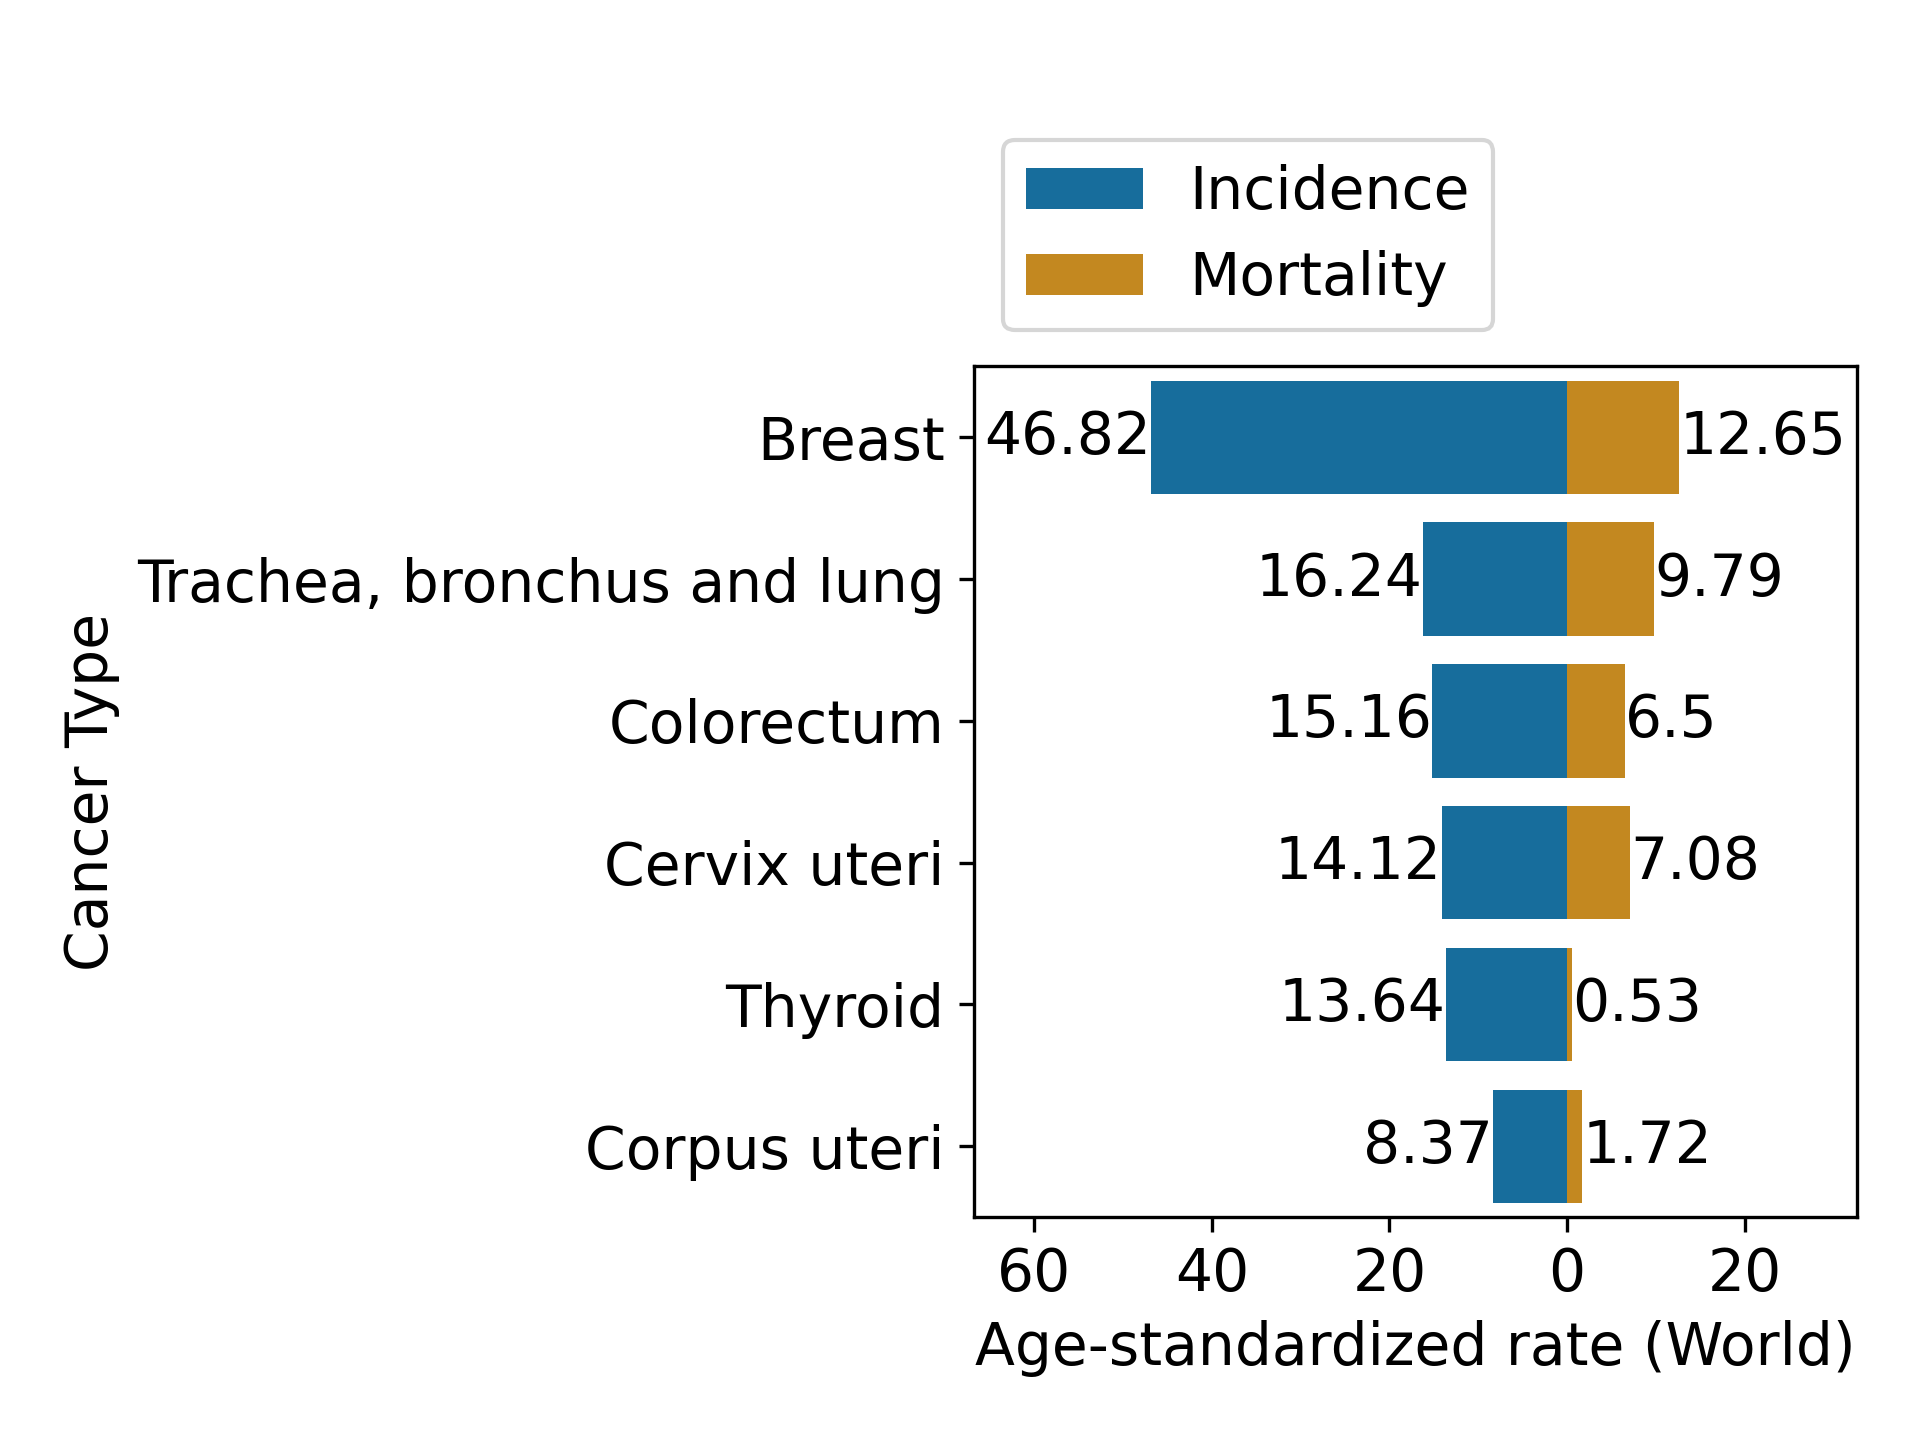
\includegraphics[width=\linewidth]{chapters/2_background/figures/bar.png}
            \caption{Incidence and mortality of cancer types}
            \label{fig:brca_bar}
        \end{subfigure} & \begin{subfigure}{0.5\textwidth} \centering

            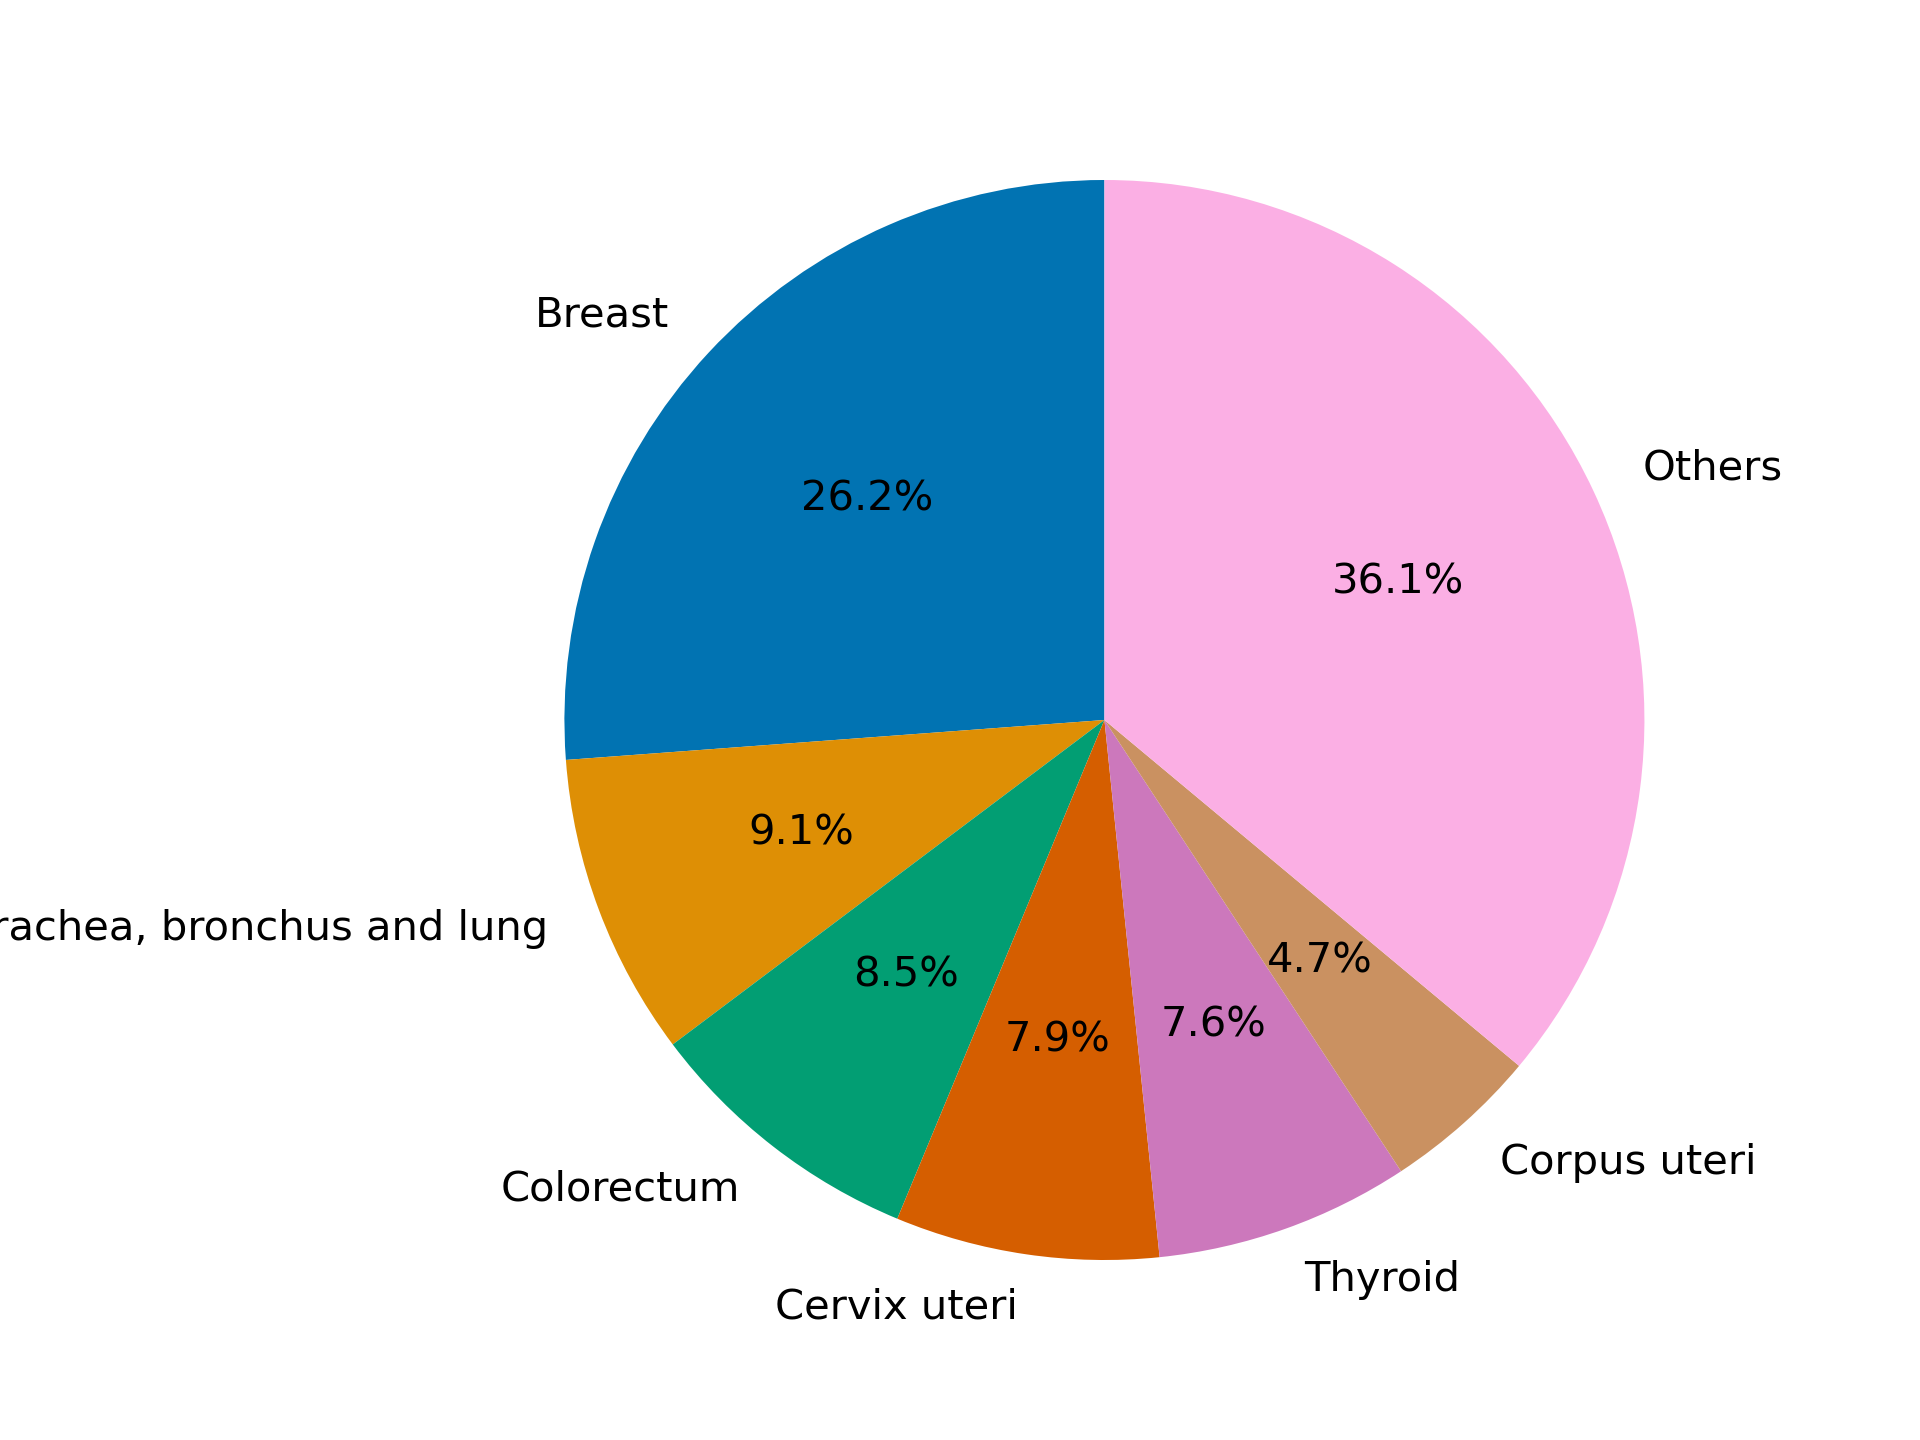
\includegraphics[width=\linewidth]{chapters/2_background/figures/pie.png}
            \caption{Relative incidence of cancer types}
            \label{fig:brca_pie}
        \end{subfigure} \end{tabular} \caption{Overview of the cancer types
        with the highest global incidence in women in 2022.
        Data were obtained from the Global Cancer Observatory
        \supercite{bray_global_2024,ferlay_global_2024}.
        Both subplots show the 6 cancer types with the highest incidence \gls{asr}.
        The numbers represent the \gls{asr} of incidence and mortality per 100,000
        individuals.
        Age standardization is necessary when comparing populations with different age
        structures\supercite{segi_age-adjusted_1960,doll_cancer_1966}.
        \textbf{a}: Absolute incidence and mortality values.
        Breast cancer is the cancer type with the highest incidence and the highest
        mortality rate with an incidence \gls{asr} of 46.82 and a mortality \gls{asr}
        of 12.65.
        \textbf{b}: Relative incidence \gls{asr} values.
        Breast cancer makes up 26.2\% of all newly diagnosed cancer cases.
    }
    \label{fig:brca_incidence_mortality} \end{figure}

Despite advancements in treatment and early detection, disparities in access to
care and late-stage diagnoses remain prevalent, particularly in low-resource
settings\supercite{wilkinson_understanding_2022,ginsburg_breast_2020}.
The mortality \gls{asr} from breast cancer is approximately 12.65 per 100,000
women per year, reflecting the ongoing challenges in managing this complex
disease \supercite{bray_global_2024,ferlay_global_2024}.
Thus, breast cancer continues to pose a formidable challenge, necessitating
concerted efforts in research, awareness, and healthcare delivery to improve
outcomes\supercite{desantis_breast_2019}.

\subsection{Types}
\label{sec:brca_types}

Breast cancer is a heterogeneous disease characterized by various subtypes that
differ in their molecular features, clinical behavior, and response to
treatment\supercite{harbeck_breast_2019}.
The classification of breast cancer is primarily based on the expression of
\glspl{hr}, such as estrogen and progesterone, and the \gls{her2}.
Understanding these subtypes is crucial for determining prognosis and tailoring
treatment strategies.
One of the most common classifications is based on hormone receptor status,
which divides breast cancer into three main categories: \gls{hr+}, \gls{her2+},
and \gls{tnbc}\supercite{clusan_basic_2023}.

\subsubsection{\Glsfmtfull{hr+}}
\gls{hr+} breast cancers express either \glspl{er} or \gls{pr} and
are typically treated with hormone therapies such as \gls{tam} or aromatase
inhibitors such as \gls{let}\supercite{geyer_molecular_2012}.
Within the \gls{hr+} category, there are further distinctions, such as luminal
A and luminal B subtypes.
Luminal A tumors are generally associated with a better prognosis and lower
proliferation rates, while luminal B tumors tend to be more aggressive and may
require chemotherapy in addition to hormone
therapy\supercite{geyer_molecular_2012}.

\subsubsection{\Glsfmtfull{her2+}}
\Gls{her2+} breast cancer is characterized by overexpression of the \gls{her2}
protein, which is associated with aggressive disease and poorer outcomes if
untreated.
However, the advent of targeted therapies, such as trastuzumab, has
significantly improved survival rates for patients with \gls{her2+} breast
cancer\supercite{modi_antitumor_2020}.
Recent studies have also identified a subset of \gls{her2}-low breast cancer,
which may not meet the criteria for \gls{her2} positivity but still expresses
low levels of the \gls{her2} protein.
This subtype has been shown to have distinct clinical outcomes and may benefit
from specific therapeutic
approaches\supercite{won_clinical_2022,mutai_prognostic_2021}.

\subsubsection{\Glsfmtfull{tnbc}}
\Gls{tnbc} is defined by the absence of \gls{er}, \gls{pr},
and \gls{her2} expression.
This subtype is known for its aggressive nature and limited treatment options,
as it does not respond to hormone therapies or \gls{her2}-targeted
therapies\supercite{sizemore_triple_2021}.
\Gls{tnbc} can be further classified into several subtypes based on gene
expression
profiles, including basal-like and claudin-low subtypes, which exhibit
different biological behaviors and responses to
treatment\supercite{lehmann_identification_2011}.
The lack of targeted therapies for \gls{tnbc} has led to ongoing research into
novel treatment strategies, including immunotherapy and combination
therapies\supercite{lehmann_identification_2011}.

\begin{table}[ht]
    \centering
    \begin{tabular}{|l|c|c|c|c|}
        \hline
                                        & \makecell{\gls{hr+}
        \\Luminal A} &
        \makecell{\gls{hr+}                                                  \\
        Luminal B}
                                        &
        \gls{her2+}
                                        & \gls{tnbc}
        \\ \hline
        Proportion of cases             & 60\%                & 10\%
                                        &
        20\%
                                        & 10\%
        \\
        \gls{er}\textalpha{} expression & ++                  & +
                                        & -
                                        & -
        \\
        PR expression                   & ++                  & +
                                        & -
                                        & -
        \\
        \gls{her2} expression           & -                   & +/-
                                        & +
                                        & -
        \\
        Proliferation (Ki67)            & Low                 & High
                                        &
        High
                                        & High
        \\
        Prognosis                       & Good                & Intermediate
                                        &
        Intermediate
                                        & Poor
        \\
        Therapy                         & Endocrine           & Endocrine

                                        &
        Anti-\gls{her2}
                                        & Chemotherapy
        \\ \hline
    \end{tabular}
    \caption{Characteristics of breast cancer
        types\supercite{clusan_basic_2023}.
        \Gls{hr+}, especially the luminal A subtype, is the most
        abundant type of breast cancer.
        \Gls{her2+} and \gls{tnbc} are less common
        but are associated with more aggressive disease and poorer outcomes.
        The table shows the main characteristics of each subtype, including \gls{hr}
        expression, \gls{her2} status, proliferation rates, prognosis, and treatment
        options.
        More information about treatment options can be found in
        \cref{sec:brca_treatment}.
    }
    \label{tab:brca_subtypes}
\end{table}

In addition to these major classifications, breast cancer can also be
categorized based on histological features, such as \gls{idc} and \gls{ilc}.
\Gls{idc} is the most common type, accounting for approximately 80\% of breast
cancer cases, while \gls{ilc} is characterized by a distinct growth pattern and
may present unique challenges in diagnosis and
treatment\supercite{mittal_molecular_nodate}.

\subsection{Causes and risk factors}
\label{sec:brca_risk-factors}

Breast cancer is a complex disease, with various causes and risk factors.
Understanding these factors is key to improving prevention, early detection,
and treatment.
These risk factors can generally be grouped into genetic, lifestyle,
environmental, and — most relevant to this thesis — hormonal
influences\supercite{clusan_basic_2023}.

\paragraph{Genetics}
Mutations in genes like BRCA1 and BRCA2 are well-known hereditary factors that
greatly increase the chances of developing breast cancer.
Women with these mutations can face a lifetime risk of up to 80\% for the
disease\supercite{jian_clinical_2017}.
Additionally, having a family history of breast cancer significantly raises the
risk, especially for first-degree relatives of those
affected\supercite{schairer_risk_2013}.

\paragraph{Lifestyle}
Diets high in fat have been linked to a higher risk, possibly because they
affect estrogen levels\supercite{turner_meta-analysis_2011}.
On the other hand, regular exercise and maintaining a healthy weight are
protective factors\supercite{claudia_admoun_etiology_2022}.
Alcohol consumption is another important factor, especially in \gls{er+} breast
cancers\supercite{bao_association_2011}.

\paragraph{Environmental factors}
Factors such as exposure to radiation or certain chemicals, can also raise the
risk of breast cancer.
For example, women who received radiation therapy to the chest for other
cancers have a significantly increased risk of developing breast cancer later
in life\supercite{froes_brandao_prolactin_2016}.
Additionally, socioeconomic status plays a role: women from lower-income
backgrounds often have less access to preventive care and early detection
services, which can lead to later diagnoses and worse
outcomes\supercite{cunningham_mind_2013}.

\paragraph{Hormonal influences}
Hormonal influences such as early menarche and late menopause increase risk
because of longer exposure to estrogen\supercite{nounu_sex_2022}.
Reproductive history is another key factor: women who have never given birth or
had their first child later in life are at a higher
risk\supercite{claudia_admoun_etiology_2022}.
Hormone replacement therapy, particularly the combined use of estrogen and
progestin, has also been linked to an increased risk of breast
cancer\supercite{turner_meta-analysis_2011}.

\begin{figure}[ht]
    \centering

    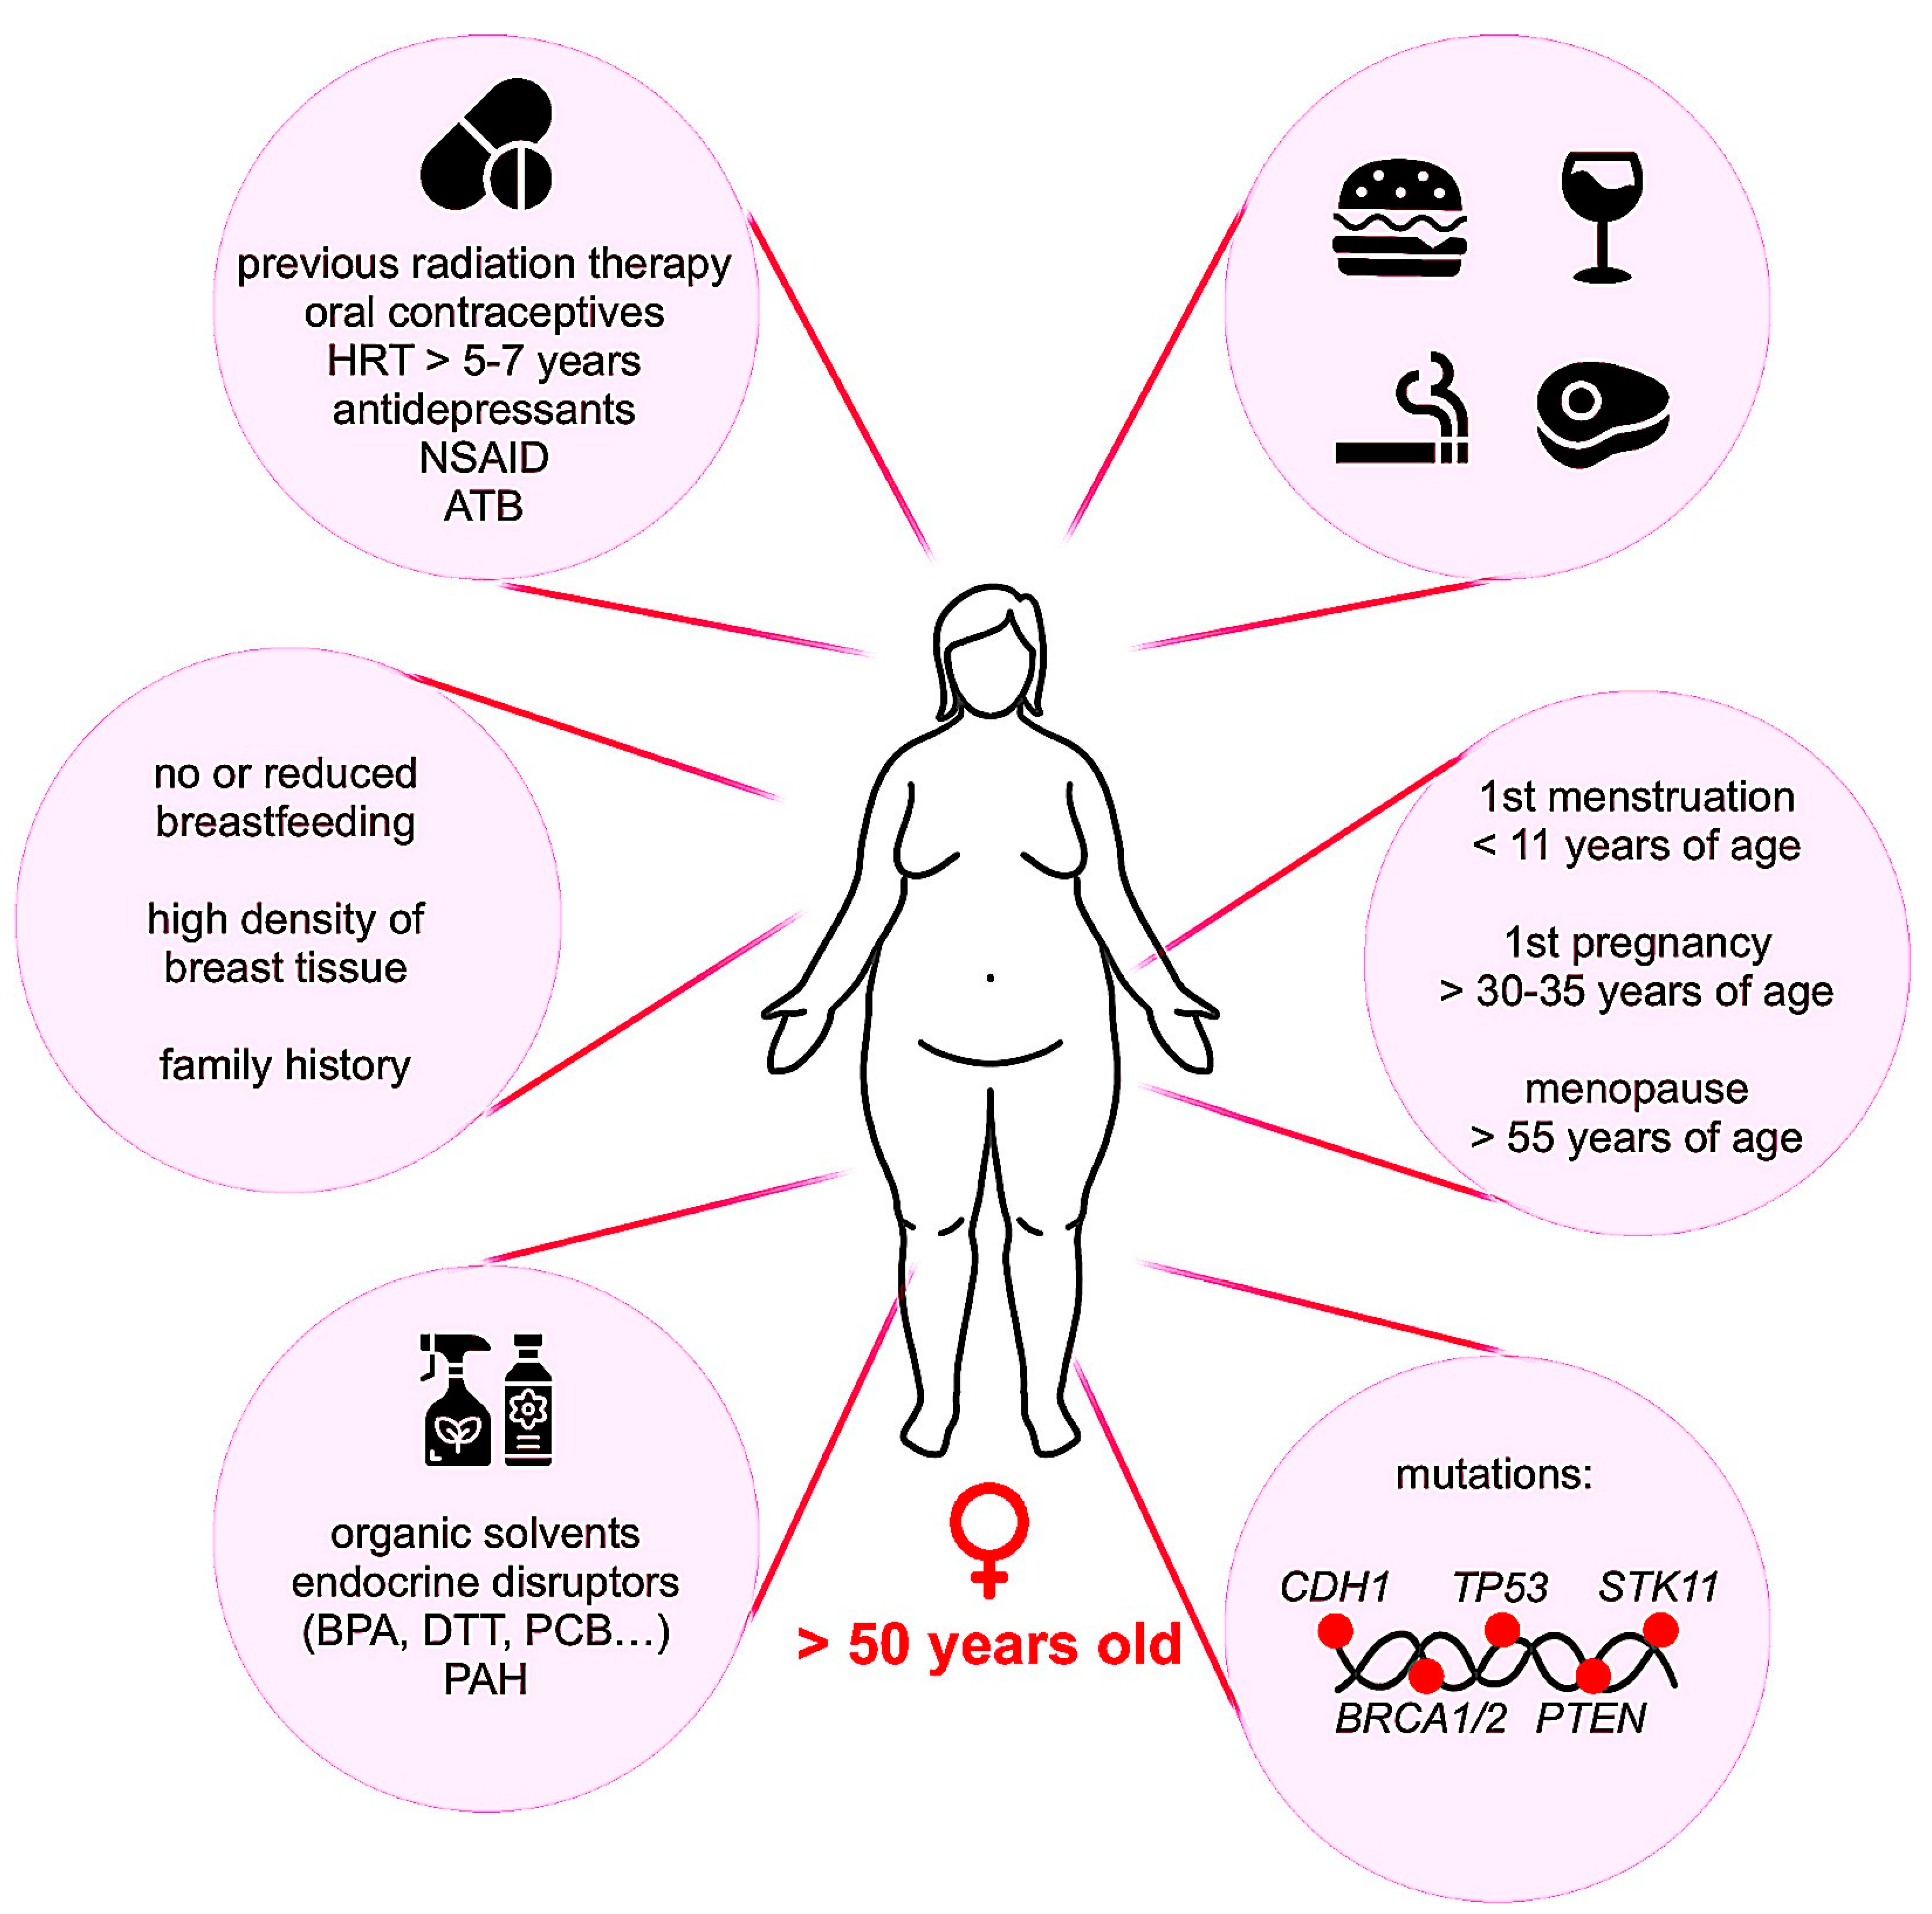
\includegraphics[width=0.5\textwidth]{chapters/2_background/figures/risk-factors.png}
    \caption{Illustration of the main risk factors for breast cancer.
        Figure was extracted from \textcite{clusan_basic_2023}.
    }
    \label{fig:brca_risk-factors}
\end{figure}

\subsection{Diagnosis}
\label{sec:brca_diagnosis}

Diagnosis of breast cancer typically involves a combination of clinical
evaluation, imaging studies, and histopathological examination.
Initial assessments often include mammography, which is a critical screening
tool that can detect tumors before they become
palpable\supercite{hameed_breast_2020}.
In cases where abnormalities are found, further imaging, such as ultrasound or
\gls{mri}, may be employed.
Definitive diagnosis is usually achieved through biopsy, where tissue samples
are collected and analyzed microscopically to confirm
malignancy\supercite{hameed_breast_2020}.
The stage at which breast cancer is diagnosed is a critical determinant of
treatment outcomes; early-stage diagnosis is associated with significantly
better prognoses\supercite{getachew_perceived_2020}.
However, barriers to early diagnosis, such as lack of awareness and access to
healthcare facilities, can lead to advanced-stage presentations, which are
linked to poorer clinical
outcomes\supercite{getachew_perceived_2020,dickens_stage_2014}.

\subsection{Treatment}
\label{sec:brca_treatment}

While type-specific treatment options have already been shown in
\cref{tab:brca_subtypes}, the choice of treatment for breast cancer is
multifaceted and depends on various factors, including the cancer subtype,
stage, and the patient's overall health.
Standard treatment modalities include surgery, radiation therapy, chemotherapy,
hormone therapy, and targeted therapies.
Surgical options may range from lumpectomy, which conserves breast tissue, to
mastectomy, which involves the removal of one or both
breasts\supercite{metcalfe_contralateral_2014,wu_breast_2014}.
Adjuvant therapies, such as chemotherapy and radiation, are often utilized to
reduce the risk of recurrence, especially in more aggressive forms like
\gls{tnbc}, which is prevalent among women with BRCA1
mutations\supercite{metcalfe_contralateral_2014}.
Hormonal therapies, such as \gls{tam} or aromatase inhibitors, are effective in
\gls{hr+} breast cancers, while targeted therapies, including \gls{her2}
inhibitors, have revolutionized treatment for \gls{her2+}
subtypes\supercite{eccles_critical_2013,pace_breast_2016}.
The choice of treatment is increasingly personalized, taking into account
genetic and epigenetic factors that may influence tumor behavior and patient
response to therapy\supercite{khakpour_methylomics_2017}.

\section{Estrogen signaling in breast cancer}
\label{sec:estrogen_signaling}

Estrogen signaling plays a pivotal role in the development and progression of
breast cancer, particularly in \gls{er+} subtypes.
The primary mechanism of action involves the binding of estrogen to \glspl{er}
(\gls{era} and \gls{erb}), which are transcription factors that regulate gene
expression associated with cell proliferation, differentiation, and survival
\supercite{misawa_estrogen-related_2015,lattouf_lkb1_2016}.
The activation of these receptors can lead to the transcription of genes that
promote tumor growth and metastasis, thereby establishing a direct link between
estrogen signaling and breast cancer pathogenesis
\supercite{feng_cross-talk_2020}.

In \gls{er+} breast cancer, estrogen signaling is often enhanced through
various intracellular signaling pathways, including the \gls{pi3k}/AKT and
\gls{mapk} pathways.
These pathways can be activated by growth factors such as \gls{her2}, which is
frequently overexpressed in aggressive breast
cancers\supercite{bratton_regulation_2010,salmeron-hernandez_bcas2_2019}.
The crosstalk between estrogen signaling and these pathways not only amplifies
the proliferative effects of estrogen but also contributes to the survival of
cancer cells under therapeutic stress, such as
chemotherapy\supercite{bratton_regulation_2010,george_hypoxia_2012}.
For instance, the interaction between \gls{era} and the \gls{pi3k}/AKT pathway
has been shown to suppress apoptosis and promote cell survival, which is
critical for tumor
progression\supercite{bratton_regulation_2010,george_hypoxia_2012}.

Moreover, the role of alternative estrogen receptors, such as \gls{era}36, has
emerged as a significant factor in breast cancer biology.
\gls{era}36 is a variant of the classical \gls{era} that mediates
rapid, non-genomic signaling responses to estrogen, influencing cell
proliferation and survival in both \gls{er+} and \gls{er-} breast cancer
cells\supercite{deng_er-36-mediated_2014,zhang_positive_2011}.
This receptor's activation can lead to enhanced sensitivity to estrogen, even
in cells that typically do not express classical estrogen receptors, thus
complicating treatment strategies\supercite{zhang_positive_2011}.

The influence of estrogen on breast cancer is further complicated by the
presence of co-regulators and other signaling molecules.
For example, the protein CAND1 has been implicated in the regulation of
estrogen signaling pathways, suggesting that it may play a role in metastasis
in \gls{er+} breast cancer\supercite{alhammad_bioinformatics_2022}.
Additionally, the interaction of estrogen with various growth factor signaling
pathways can lead to the upregulation of genes associated with cancer stem cell
properties, thereby promoting tumor heterogeneity and resistance to
therapies\supercite{fillmore_estrogen_2010,xue_sox9fxyd3src_2019}.

\subsection{Important genes}
\label{sec:important_genes}

The following genes are essential components of the estrogen signaling pathway.
While there are many other genes involved in this pathway, these two genes have
been genetically modified in the datasets used in this thesis.
Further details on the genetic modifications can be found in
\cref{sec:datasets}.

\subsubsection{\Glsfmtfull{cyp19}}
The \gls{cyp19} gene encodes the aromatase enzyme, which is essential for the
biosynthesis of estrogens from androgens (such as testosterone), playing a
pivotal role in estrogen signaling and breast cancer development.
Elevated \gls{cyp19} expression has been linked to poor survival outcomes in
\gls{er+} breast cancer patients, with high levels correlating with increased
metastasis and recurrence
rates\supercite{barros-oliveira_cyp19a1_2020,friesenhengst_elevated_2018}.
Genetic polymorphisms in \gls{cyp19}, such as the rs936306 C/T variant, have
been associated with variations in circulating estradiol levels, influencing
breast cancer risk\supercite{ghosh_potential_2012}.
Furthermore, \gls{cyp19} expression is regulated by various factors, including
\gls{fsh}, which enhances its transcription in granulosa cells, thereby
promoting estrogen
synthesis\supercite{savolainen-peltonen_estrogen_2018,li_microrna-7a2_2022}.
Dysregulation of \gls{cyp19} can lead to aberrant estrogen levels, contributing
to tumorigenesis and resistance to endocrine
therapies\supercite{dabydeen_comparison_2015}.
Thus, \gls{cyp19} serves as both a critical enzyme in estrogen biosynthesis and
a potential therapeutic target in breast cancer management.

\subsubsection{\Glsfmtfull{esr1}}
\label{sec:esr1}
The \gls{esr1} gene encodes the \gls{era} protein, which - as mentioned above -
is a critical regulator of estrogen signaling in breast cancer.
\Gls{esr1} mutations and amplifications are associated with resistance to
endocrine
therapies, such as \gls{tam}, complicating treatment
outcomes\supercite{aguilar_biological_2010,jeselsohn_emergence_2014}.
Notably, \gls{esr1} mutations can lead to constitutively active receptors that
drive tumor growth independent of estrogen\supercite{toy_activating_2017}.
Additionally, \gls{esr1}'s expression is modulated by various factors,
including \glspl{mirna} and transcription factors, which can influence the
cancer phenotype and therapeutic responses\supercite{mansoori_mir-142-3p_2019}.
The gene's regulatory mechanisms, including chromatin remodeling and enhancer
activity, further illustrate its complex role in breast cancer
biology\supercite{powers_proteasome_2013,tomita_cluster_2015}.
Thus, \gls{esr1} serves as both a biomarker for prognosis and a target for
therapeutic intervention in \gls{er+} breast cancer.

\subsection{Important treatment agents}
\label{sec:important_treatments}

The following treatment agents are commonly used in the management of \gls{er+}
breast cancer.
They are of special relevance in this study, as they have been administered to
some cohorts of the mouse models analyzed in the used datasets.
Details on the treatment regimens can be found in \cref{sec:datasets}.

\subsubsection{\Glsfmtlong{tam}}

Tamoxifen is a \gls{serm} that plays a crucial role in the management of
estrogen \gls{er+} breast cancer.
By competing with estrogen for binding to the \gls{er}, \gls{tam} inhibits the
proliferation of breast cancer cells that rely on estrogen signaling for
growth\supercite{radhi_tamoxifen_2023}.
This mechanism is particularly significant as approximately 70\% of breast
cancers express \gls{er}, making \gls{tam} a cornerstone of endocrine therapy
for these patients\supercite{wang_induced_2019}.
Additionally, \gls{tam} has been shown to induce apoptosis in \gls{er+} cancer
cells, further contributing to its anticancer
effects\supercite{li_tamoxifen_2017}.

Despite its efficacy, \gls{tam} resistance remains a significant challenge,
affecting nearly 40\% of patients\supercite{tuttle_novel_2012}.
Resistance mechanisms are multifaceted, involving alterations in estrogen
signaling pathways, cell cycle regulation, and growth factor receptor
pathways\supercite{zhuang_p21-activated_2015,mills_mechanisms_2018}.
Furthermore, \gls{tam}'s effects can vary depending on the tissue context,
exhibiting antiestrogenic properties in breast tissue while acting as an
estrogen agonist in other tissues\supercite{jovanovska_effects_2021}.
This duality underscores the complexity of \gls{tam}'s role in breast cancer
treatment and the need for ongoing research to overcome resistance and optimize
therapeutic strategies.

\subsubsection{\Glsfmtlong{let}}

\Gls{let} is a third-generation non-steroidal aromatase inhibitor that plays a
significant role in estrogen signaling and the treatment of estrogen \gls{er+}
breast cancer.
By inhibiting the aromatase enzyme, \gls{let} effectively reduces estrogen
production, leading to decreased estrogen levels in the body, which is crucial
for the growth of \gls{er+} tumors\supercite{priyadarsini_quality_2022}.
This mechanism of action is particularly beneficial for postmenopausal women,
as it targets the primary source of estrogen in this population—adrenal and
peripheral conversion of androgens to
estrogens\supercite{priyadarsini_quality_2022}.

Clinical studies have demonstrated that \gls{let} is more effective than
\gls{tam} in certain settings, particularly in the adjuvant treatment of
early-stage breast cancer, where it has been associated with improved
disease-free survival rates\supercite{jerusalem_continuous_2021}.
However, some tumors may develop resistance to \gls{let}, often linked to the
expression of estrogen-regulated genes and the tumor's hormonal environment
\supercite{lee_suppressed_2021}.
Furthermore, \gls{let}'s efficacy can be influenced by the presence of other
hormonal receptors, such as progesterone receptors, which may modulate the
tumor's response to treatment \supercite{lee_suppressed_2021}.
Overall, \gls{let} represents a critical advancement in endocrine therapy for
breast cancer, particularly for patients with \gls{er+} tumors.

\section{Gene Expression}
\label{sec:gene_expression}

Gene expression is a complex process consisting of multiple steps that
culminate in the production of functional proteins.
This process is tightly regulated at various levels to ensure the accurate and
timely expression of genes in response to internal and external signals.
Here, I provide an overview of the key steps involved in gene expression,
focusing on the transcription and processing of pre-\gls{mrna} into mature
\gls{mrna}.

\subsection{Transcription and pre-\glsfmtshort{mrna} formation}
Gene expression begins with transcription, where \gls{rna} polymerase II
synthesizes a primary transcript of \gls{rna} from the \gls{dna} template.
This primary transcript, known as pre-\gls{mrna}, contains both exons (coding
sequences) and introns (non-coding sequences)\supercite{lee_mechanisms_2015}.
The pre-\gls{mrna} undergoes several modifications before it can be translated
into a protein.

\subsection{Capping and Polyadenylation}
One of the first modifications to occur during pre-\gls{mrna} processing is the
addition of a 5' cap, which consists of a modified guanine nucleotide.
This cap is crucial for \gls{mrna} stability, nuclear export, and initiation of
translation\supercite{topisirovic_cap_2011}.
Following transcription, the pre-\gls{mrna} is also polyadenylated at its 3'
end, where a stretch of adenine nucleotides is added.
This poly(A) tail enhances \gls{mrna} stability and facilitates its export from
the nucleus to the cytoplasm\supercite{passmore_roles_2022}.

\subsection{Splicing}
The splicing of pre-\gls{mrna} is a critical step that involves the removal of
introns and the joining of exons to form a continuous coding sequence.
This process is catalyzed by the spliceosome, a large and dynamic
ribonucleoprotein complex composed of \gls{snrna} and numerous protein
factors\supercite{lee_mechanisms_2015}.
The spliceosome recognizes specific sequences at the exon-intron boundaries,
facilitating the precise excision of introns and ligation of
exons\supercite{wang_splicing_2008}.

\subsubsection{Alternative Splicing}
A significant aspect of pre-\gls{mrna} processing is alternative splicing,
which allows a single gene to produce multiple \gls{mrna} isoforms by including
or excluding specific exons.
This process is regulated by various splicing factors that interact with
cis-acting elements in the
pre-\gls{mrna}\supercite{le_alternative_2015,murphy_therapeutic_2022}.
Approximately 95\% of human genes with multiple exons undergo alternative
splicing, contributing to the diversity of the proteome and enabling cells to
adapt to different physiological conditions\supercite{le_alternative_2015}.
The regulation of alternative splicing is influenced by the abundance and
activity of splicing factors, which can change in response to cellular
signals\supercite{wang_mechanism_2015}.

\subsection{Nuclear Export}
Once splicing is complete, the mature \gls{mrna}, now devoid of introns and
containing a 5' cap and a poly(A) tail, is exported from the nucleus to the
cytoplasm.
This export is facilitated by the nuclear cap-binding complex and other
\glspl{rbp} that ensure the \gls{mrna} is properly processed and ready for
translation\supercite{soucek_evolutionarily_2016}.

\section{Circular RNAs (circRNAs)}

CircRNAs represent a novel class of non-coding RNAs that have garnered
significant attention in recent years due to their unique structural properties
and diverse biological functions.
Unlike linear RNAs, circRNAs are characterized by a covalently closed loop
structure, which confers increased stability and resistance to degradation by
exonucleases, making them reliable biomarkers and potential therapeutic targets
in various
diseases\supercite{ma_circular_2020,hoque_exploring_2023,wilusz_circular_2017}.
Initially considered mere byproducts of mRNA splicing, circRNAs have now been
recognized for their regulatory roles in gene expression, cellular processes,
and disease mechanisms\supercite{cherubini_foxp1_2019,wilusz_360_2018}.

\subsection{Biogenesis}
During standard gene expression, pre-mRNA is transcribed from DNA.
Splicing then removes introns and joins exons to produce mature
mRNA\supercite{black_mechanisms_2003}.
In conventional splicing, an upstream 5' splice site (donor) connects to a
downstream 3' splice site (acceptor), forming linear mRNA
(\cref{fig:circRNA_splicing}a).
Conversely, for circRNAs, a downstream 5' splice site connects to an upstream
3' splice site in reverse order across at least one
exon\supercite{chen_expanding_2020}.
This backsplicing process is - just like conventional splicing - catalyzed by
the canonical spliceosome\supercite{starke_exon_2015} and results in a circular
RNA molecule (\cref{fig:circRNA_splicing}b).

\subsubsection{Models}

Circular RNAs (circRNAs) are generated through two primary models of
biogenesis: the direct backsplicing model and the lariat-intermediate model.
The direct backsplicing model involves the covalent joining of a downstream 5'
splice site to an upstream 3' splice site, resulting in a circular structure
devoid of a poly(A) tail and 5' cap, which distinguishes circRNAs from linear
RNAs\supercite{zhang_complementary_2014,ferreira_circular_2018}.
This model emphasizes the role of complementary sequences in the introns
flanking the exons, which facilitate the proximity of splice sites necessary
for backsplicing\supercite{zhang_complementary_2014,meganck_engineering_2021}.

In contrast, the lariat-intermediate model posits that circRNAs can also arise
from lariat structures formed during canonical splicing.
In this scenario, introns are excised as lariats, and the remaining exons can
circularize, leading to circRNA
formation\supercite{humphreys_ularcirc_2019,barrett_circular_2015}.
This model highlights the potential for exon skipping, where certain exons are
omitted during splicing, further contributing to circRNA
diversity\supercite{sun_microarray_2020,barrett_circular_2015}.
Both models underscore the complexity of circRNA biogenesis and the interplay
of various molecular mechanisms involved in their
formation\supercite{sharma_recent_2021}.

% TODO: Reference {fig:circRNA_splicing}d

\subsubsection{Alternative splicing}
In conventional splicing, introns are removed and exons are joined linearly.
However, in some cases, exons are skipped or introns are retained, leading to
alternative mature mRNA transcripts based on the same pre-mRNA.
This process is known as alternative splicing\supercite{nilsen_expansion_2010}.
Similarly, circRNAs can be subject to alternative splicing.
This can result in the structures shown in \cref{fig:circRNA_splicing}e and
\cref{fig:circRNA_splicing}f.

\begin{figure}[ht]
    \centering

    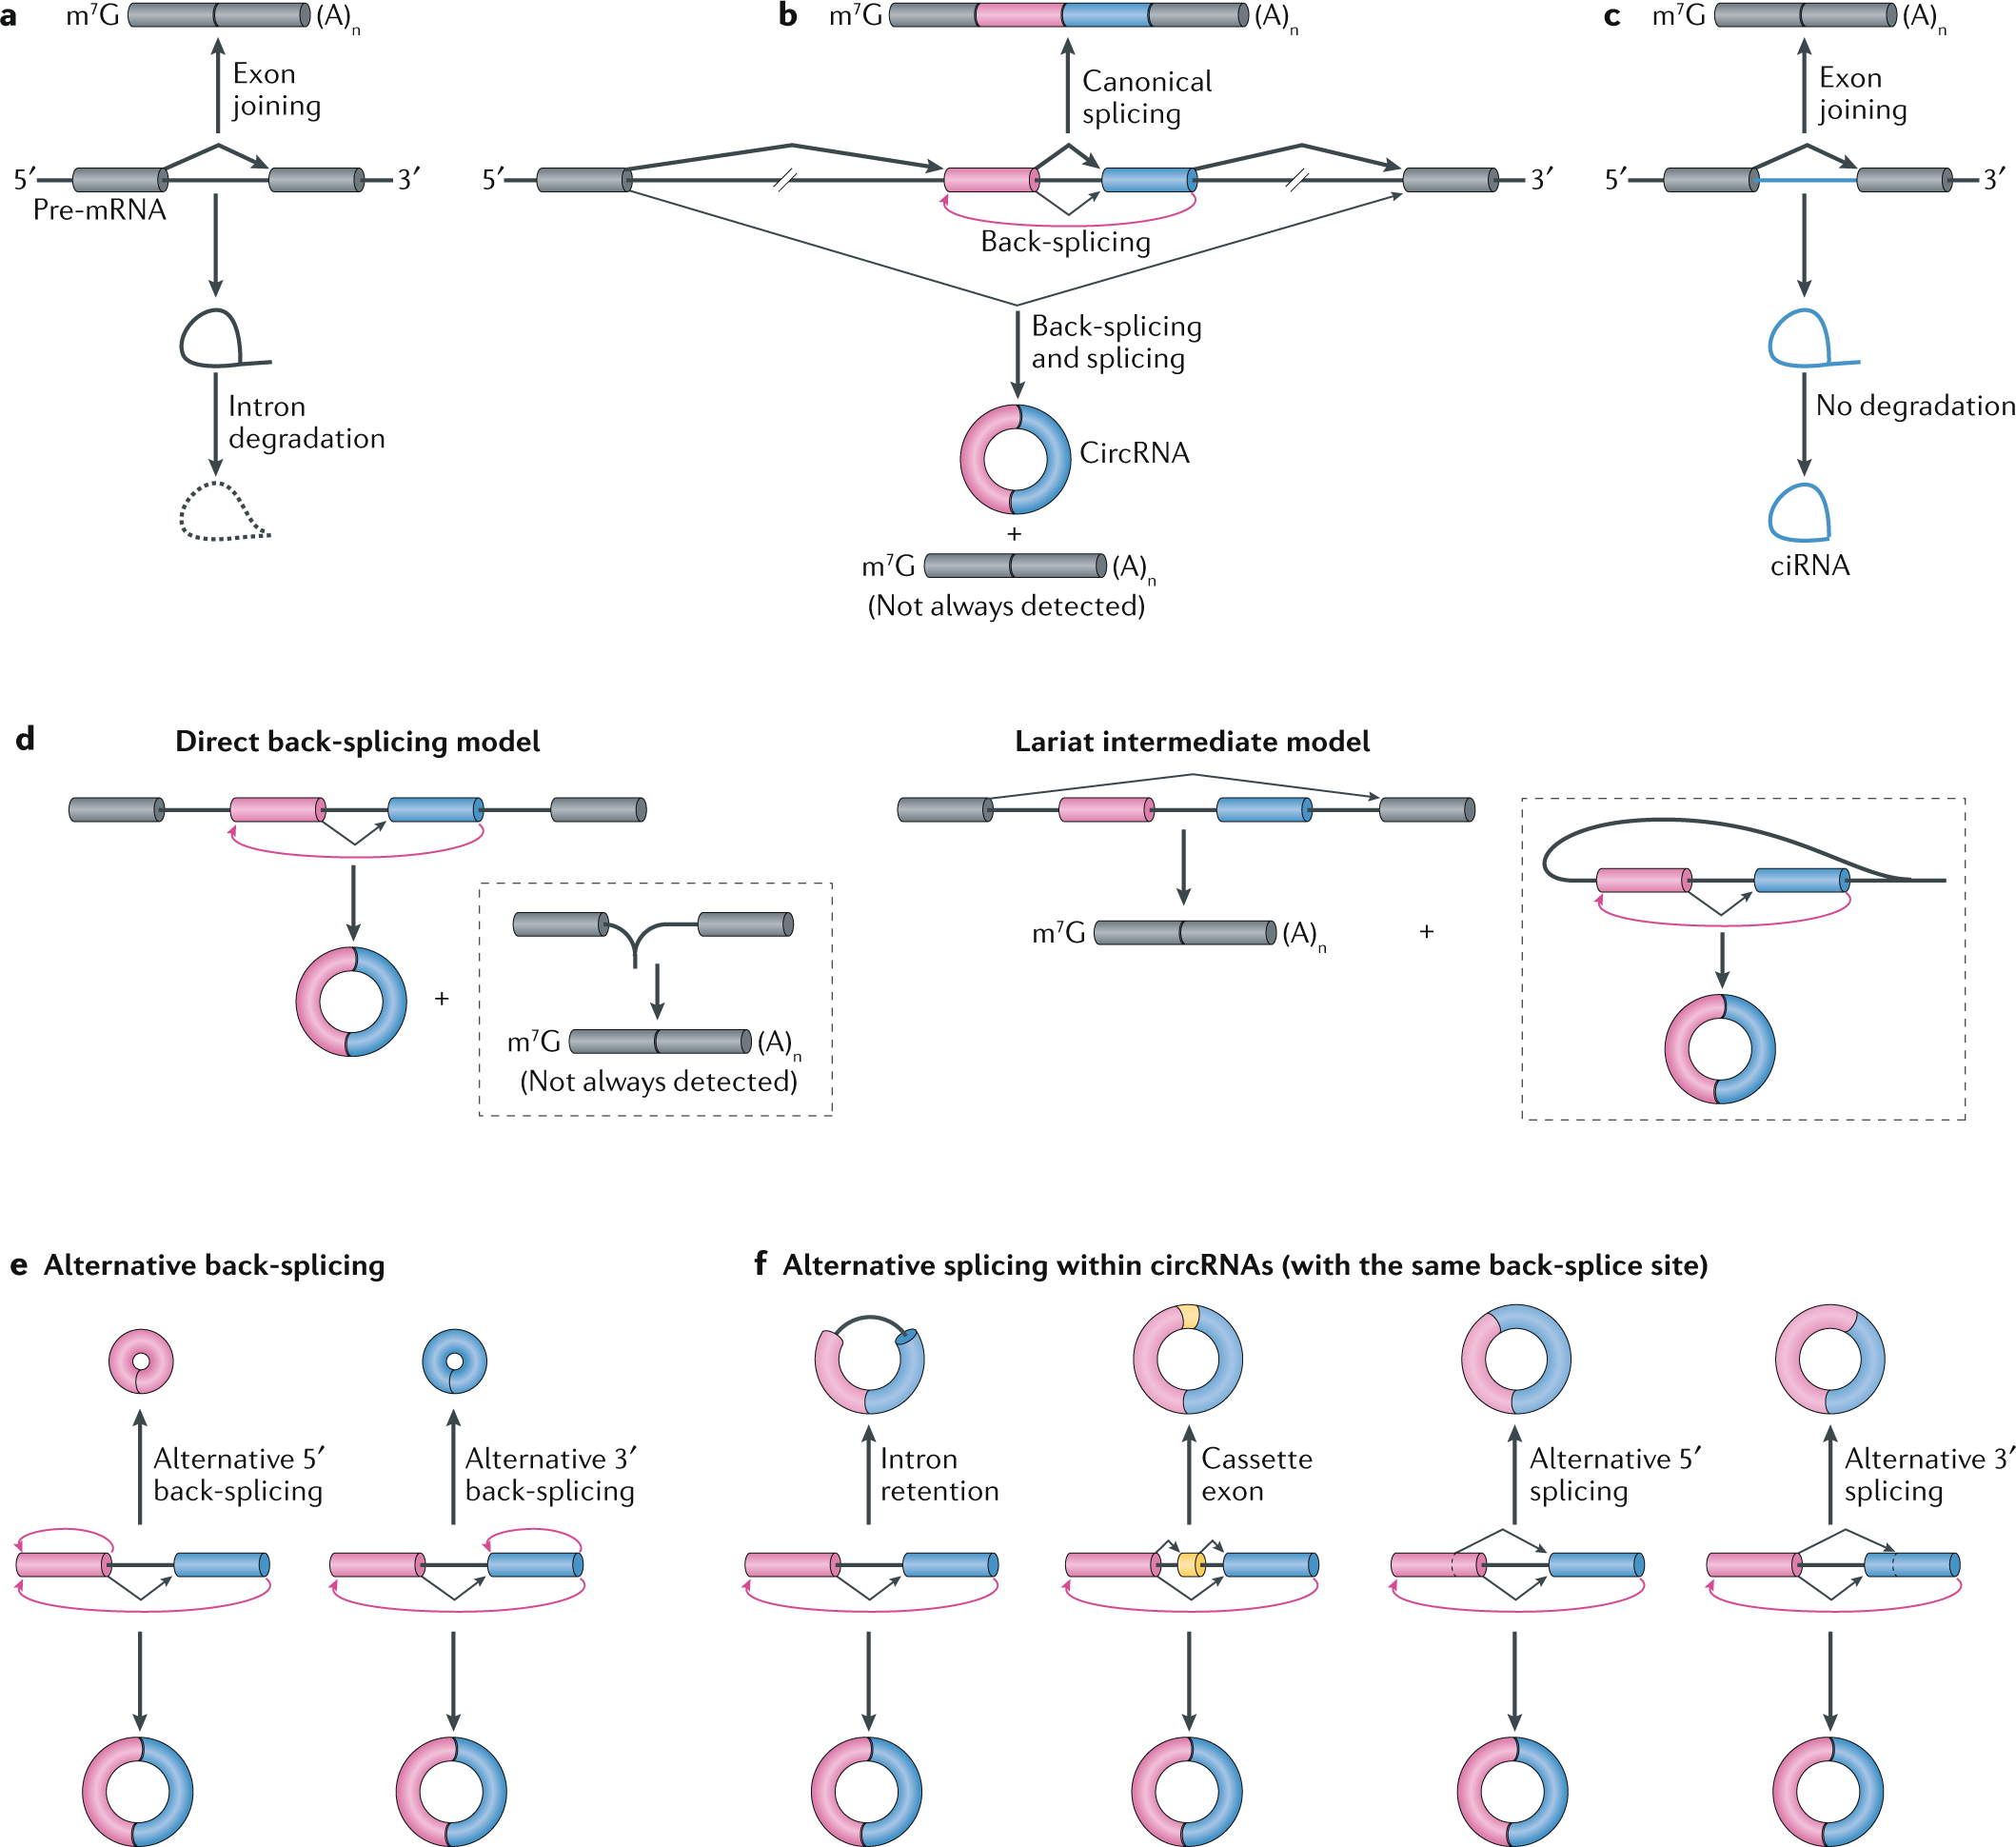
\includegraphics[width=\textwidth]{chapters/2_background/figures/circRNA-splicing.png}
    \caption{Splicing of circRNAs} % TODO: Add detailed caption
    \label{fig:circRNA_splicing}
\end{figure}

\subsection{circRNA types}
\iffalse
    \subsubsection{Circular intronic RNAs (ciRNAs)}
    Introns typically form a lariat shape during conventional splicing, which is
    generally debranched and degraded soon after splicing
    (\cref{fig:circRNA_splicing}a).
    However, in some cases, introns evade debranching and instead form covalently
    bonded circular RNA molecules (\cref{fig:circRNA_splicing}c), known as circular
    intronic RNAs (ciRNAs) \supercite{chen_expanding_2020,zhang_circular_2013}.

    \subsubsection{Exonic circular RNAs (EcircRNAs)}
    EcircRNAs are generated from exon-skipping events.
    Here, the lariat contains at least one exon and potentially multiple introns.
    The introns are subsequently removed through internal splicing, producing a
    circular RNA molecule composed solely of exonic sequences
    \supercite{xiao_circular_2022, li_biogenesis_2018}.

    \subsubsection{Exon-intron circular RNAs (EIcircRNAs)}
    The formation of EIcircRNAs is similar to that of EcircRNAs, with the exception
    that introns are not completely removed during splicing, resulting in a
    circular RNA molecule containing both exonic and intronic sequences
    \supercite{xiao_circular_2022}.
\fi

\paragraph{Exonic circular RNAs (ecircRNAs)} are the most prevalent type of
circRNAs, primarily formed from back-splicing of exons from protein-coding
genes.
They are typically located in the cytoplasm and can function as sponges for
microRNAs (miRNAs), thereby modulating gene expression and influencing various
cellular processes, including tumorigenesis and cellular differentiation
(Bachmayr-Heyda et al., 2015; Wang et al., 2021).
EcircRNAs have been shown to interact with RNA-binding proteins, which can
further regulate their stability and function (Zang et al., 2018).
Their abundance and stability make them potential biomarkers for various
diseases, including cancers (Li et al., 2021; Wang et al., 2021).

\paragraph{Intronic circular RNAs (ciRNAs)}, on the other hand, are derived
from introns
and are predominantly localized in the nucleus.
They play a role in regulating the transcription of their parental genes and
are characterized by their constrained expression patterns (Ma et al., 2020;
Xie et al., 2023).
ciRNAs are
believed to interact with components of the transcription machinery, thereby
influencing gene expression at the transcriptional level (Reddy et al., 2017).
The nuclear localization of ciRNAs suggests they may have distinct regulatory
functions compared to their ecircRNA counterparts.

\paragraph{Exon-Intron Circular RNAs (EIciRNAs)} are a hybrid form that
includes both
exonic and intronic sequences.
Like ciRNAs, EIciRNAs are also found in the nucleus and have been implicated in
the regulation of gene transcription.
They can enhance the expression of their parent genes by interacting with RNA
polymerase II and other transcription factors (Chen et al., 2022; Su, 2024).
This dual composition allows EIciRNAs to potentially serve as intermediaries in
the regulation of gene expression, bridging the functions of both ecircRNAs and
ciRNAs.

\paragraph{Intergenic circular RNAs (IcircRNAs)} are formed from regions of the
genome
that do not code for proteins and are often less characterized than the other
types.
Their functions remain largely unknown, but they are thought to contribute to
the regulatory networks within cells, possibly by interacting with other RNA
molecules or proteins (Li et al., 2021).
The study of IcircRNAs is still in its infancy, and further research is needed
to elucidate their roles in cellular processes.

\subsection{Biological functions}
circRNAs have emerged as key players in various biological processes,
showcasing
a wide range of functions that contribute substantially to cellular regulation.

\subsubsection{Micro RNA sponging}
One of the most well-documented functions of circRNAs is their ability to act
as miRNA sponges.
This mechanism involves the binding of circRNAs to specific miRNAs, thereby
preventing these miRNAs from interacting with their target mRNAs.
For instance, the circRNA CDR1as has been shown to contain over 60 binding
sites for miR-7, effectively sequestering it and allowing the expression of
miR-7 target genes to
increase\supercite{guo_expanded_2014,yuan_regulatory_2020}.
This competitive endogenous RNA (ceRNA) activity is crucial in regulating gene
expression and has been implicated in various cancers, including gliomas and
gynecological cancers\supercite{dong_expression_2020,song_circular_2016}.
Additionally, circRNAs such as circ-0000437 have been identified as sponges for
miRNAs involved in tumor progression, highlighting their potential as
therapeutic targets\supercite{li_peptide_2021,cui_circular_2022}.

\subsubsection{Protein interactions}
Beyond miRNA sponging, circRNAs also participate in protein interactions.
They can serve as scaffolds for RNA-binding proteins (RBPs), influencing
various cellular processes, including transcription and
splicing\supercite{li_comprehensive_2017,qu_emerging_2017}.
For example, circRNAs can recruit RBPs to specific genomic loci, thereby
modulating the transcriptional landscape of the
cell\supercite{li_comprehensive_2017}.
This interaction can lead to the regulation of gene expression at multiple
levels, further emphasizing the multifaceted roles of circRNAs in cellular
biology\supercite{zhang_important_2024,he_targeting_2021}.
Moreover, some circRNAs have been shown to interact with proteins that are
involved in signaling pathways, such as the Wnt/\textbeta{}-catenin pathway,
thereby influencing cellular proliferation and
differentiation\supercite{peng_novel_2021}.

\subsubsection{Translation into peptides}
In the canonical initiation of translation, ribosomes bind to the 5' cap of an
mRNA \supercite{hinnebusch_mechanism_2012}.
Because circRNAs are circular and lack a 5' cap, they were long thought to be
non-coding \supercite{bao_regulatory_2019,greene_circular_2017}.
However, research has shown that circRNAs with internal ribosome entry sites
can indeed be translated into proteins \supercite{chen_expanding_2020}:

\paragraph{Internal ribosome entry sites (IRES)} In 1988, researchers
discovered that certain viral and cellular mRNAs contain sequences allowing
ribosomes to initiate translation without a 5' cap
\supercite{pelletier_internal_1988, jang_segment_1988}.
These sequences are known as internal ribosome entry sites (IRES).
In 1995, Chen and Sarnow demonstrated that artificially engineered circRNAs
containing an IRES sequence are translated into peptides
\supercite{chen_initiation_1995}.
Later, it was found that some circRNAs naturally possess IRES sequences and can
thus be translated into peptides
\supercite{chen_expanding_2020,legnini_circ-znf609_2017,pamudurti_translation_2017}.
A concrete example for an IRES is the consensus motif for
N\textsuperscript{6}-methyladenosine modification
\supercite{yang_extensive_2017}.

\paragraph{N\textsuperscript{6}-methyladenosine (m\textsuperscript{6}
    A)}  m\textsuperscript{6}A is the most abundant base modification in eukaryotic
RNA \supercite{yang_extensive_2017,li_pivotal_2014,wei_methylated_1975}.
% General introduction to m6A
Research has shown that m\textsuperscript{6}A modification can affect
localization, splicing, translation and degradation of RNA molecules
\supercite{yue_rna_2015,meyer_dynamic_2014}.
The effect of m\textsuperscript{6}A modification on translation is particularly
interesting, as it has been shown that m\textsuperscript{6}A modifications in
3' UTRs can enhance translation
efficiency\supercite{wang_n6-methyladenosine_2015}, while m\textsuperscript{6}A
modifications in 5' UTRs can promote cap-independent translation, especially in
heat shock stress\supercite{zhou_dynamic_2015,meyer_5_2015}.

% Build bridge to IRES-dependent mechanism
m\textsuperscript{6}
A modifications mostly occur in the consensus motif RRm\textsuperscript{6}ACH
(R = purine, H = non-guanine base)
\supercite{csepany_sequence_1990,harper_sequence_1990}, which has been found to
be enriched in circRNAs \supercite{yang_extensive_2017}.
In circRNAs, a single m\textsuperscript{6}A modification is often enough to
initiate translation\supercite{yang_extensive_2017}.

\subsection{Potential applications}
The unique properties of circRNAs, such as their stability, abundance, and
specific expression patterns, make them attractive candidates for various
applications in the field of molecular biology and medicine.
Their potential uses include serving as biomarkers for disease diagnosis and
prognosis, therapeutic targets for drug development, and tools for gene
regulation and editing.

\subsubsection{Biomarkers}
One of the most compelling applications of circRNAs lies in their potential as
biomarkers for cancer diagnosis and prognosis.
Studies have demonstrated that circRNAs can serve as reliable indicators of
tumor progression and treatment response.
For instance, circRNAs exhibit higher expression levels in certain cancers
compared to their linear counterparts, suggesting their utility in liquid
biopsies for non-invasive cancer
monitoring\supercite{bao_prognostic_2020,ren_construction_2017}.
Their stability in bodily fluids such as plasma and saliva further enhances
their applicability as biomarkers, as they are less prone to degradation than
traditional RNA markers\supercite{bao_prognostic_2020,zhang_circular_2018}.
Specific circRNAs, such as hsa\_circ\_0000190, have been correlated with
advanced stages of lung cancer, indicating their potential role in clinical
settings\supercite{luo_plasma_2020}.
Moreover, circRNAs have been implicated in chemoresistance, providing insights
into treatment efficacy and patient
management\supercite{geng_function_2018,feng_functions_2019}.

Beyond their role in cancer, circRNAs are also being explored in the context of
autoimmune diseases and neurological disorders.
For example, circRNAs have been identified as novel biomarkers for rheumatoid
arthritis and multiple sclerosis, highlighting their versatility in reflecting
disease states beyond
oncology\supercite{ouyang_identification_2021,he_exosomal_2019}.
Their expression profiles in various tissues suggest that circRNAs may play a
role in the pathophysiology of these conditions, potentially guiding
therapeutic strategies\supercite{mohammed_circular_2023}.

\subsubsection{Therapeutic targets}
In addition to their diagnostic potential, circRNAs are being investigated as
therapeutic targets.
Their ability to modulate gene expression and interact with microRNAs positions
them as key regulators in cellular processes, including those involved in
cancer stem cell dynamics and immune responses\supercite{cheng_emerging_2023}.
Emerging research indicates that circRNAs can be engineered for therapeutic
purposes, such as enhancing the efficacy of RNA-based therapies like CRISPR and
siRNA\supercite{wesselhoeft_engineering_2018}.
This opens avenues for innovative treatment strategies that leverage the unique
properties of circRNAs to combat diseases more effectively.

\section{Sequencing \gls{crna}s}

Sequencing technologies have revolutionized the field of molecular biology,
enabling researchers to explore the complexities of the genome and
transcriptome with unprecedented depth and accuracy.
Traditionally, RNA sequencing (RNA-Seq) has been performed following poly-A
enrichment, a method that selectively isolates polyadenylated mRNA transcripts.
This approach, however, poses significant challenges for the study of circular
RNAs (\gls{crna}s), which lack 5' caps and poly-A tails, rendering them
undetectable in conventional sequencing protocols\supercite{guo_expanded_2014}.
As a result, \gls{crna}s have often been overlooked in transcriptomic analyses,
leading to an incomplete understanding of their biological roles and regulatory
mechanisms.

\subsection{Total RNA sequencing (total-RNA-Seq)}
The advent of total-RNA-Seq has paved the way for a more comprehensive
investigation of \gls{crna}s.
Unlike poly-A enrichment methods, total-RNA-Seq captures all RNA species,
including non-coding RNAs such as \gls{crna}s, thereby providing a more
holistic view of the transcriptome\supercite{panda_identification_2017}.
This technique has facilitated the identification of numerous \gls{crna}s
across various species and tissues, revealing their high abundance and
stability compared to linear RNA
counterparts\supercite{liu_circular_2016,cao_expression_2018}.
For instance, studies have shown that \gls{crna}s can be expressed at levels
significantly higher than their linear isomers, highlighting their potential
functional significance in cellular processes\supercite{liu_circular_2016}.

\section{State of the art}
\Glspl{crna} have emerged as significant players in the
molecular landscape of breast cancer, particularly in relation to estrogen
signaling and tumor progression.
They have been implicated in various cellular processes, including the
regulation of gene expression and the modulation of signaling pathways
associated with cancer
development\supercite{li_circrna-sfmbt2_2023,tran_new_2020}.
The dysregulation of \glspl{crna} has been observed in breast cancer, where
they can act as \glspl{cerna}, sponging \glspl{mirna} and thereby influencing
the expression of target \glspl{mrna} involved in critical pathways such as
\gls{er} signaling\supercite{nair_circular_2016,xu_circrna_2022}.

\subsection{\Glsfmtshortpl{crna} in breast cancer}
Recent studies have highlighted specific \glspl{crna} that are associated with
breast cancer subtypes and their clinical implications.
For instance, \gls{crna}-SFMBT2 has been shown to orchestrate
\gls{er}\textalpha{} activation, contributing to \gls{tam} resistance in breast
cancer cells, thereby underscoring the role of \glspl{crna} in therapeutic
resistance\supercite{li_circrna-sfmbt2_2023}.
Additionally, \glspl{crna} such as circTADA2As and circFBXL5 have been
identified as regulators of \glspl{mirna} that target key signaling pathways,
including the SOCS3 and MAPK/ERK pathways, which are crucial for cell
proliferation and metastasis in breast
cancer\supercite{xu_circtada2as_2019,gao_hsa_circrna_0006528_2019}.
This suggests that \glspl{crna} not only participate in the pathogenesis of
breast cancer but also serve as potential biomarkers for diagnosis and
prognosis\supercite{liu_influence_2021,chen_circepsti1_2018}.

\subsection{\Glsfmtshortpl{crna} in estrogen signaling}
The interaction between \glspl{crna} and estrogen signaling is particularly
noteworthy.
Research has demonstrated that \gls{er+} breast cancer subtypes exhibit
specific \gls{crna} expression profiles that overlap with genes involved in
estrogen signaling pathways\supercite{nair_circular_2016}.
For example, \gls{crna}-000911 has been shown to suppress breast cancer cell
proliferation and invasion by sponging miR-449a, which in turn activates the
Notch1 signaling pathway, a known mediator of estrogen
signaling\supercite{wang_comprehensive_2018}.
Furthermore, the \gls{crna}-\gls{mirna}-\gls{mrna} regulatory networks
constructed in various studies have revealed that \glspl{crna} can modulate the
expression of genes related to estrogen response, oxidative stress, and
epigenetic modifications, thereby influencing tumor behavior and patient
outcomes\supercite{xu_circrna_2022,nair_circular_2016}.


\chapter{Materials and Methods}
\label{chap:materials_and_methods}

\section{Data}
\label{sec:data}

\subsection{\Glsfmtfullpl{gemm}}
\label{sec:mouse_models}
\glsunset{gemm}
Mouse models play a crucial role in breast cancer research, offering a powerful
tool for understanding the molecular mechanisms of disease development and
progression.
\Glspl{gemm} allow researchers to manipulate specific genes, such as those
involved in estrogen signaling\supercite{park_mouse_2018}.
These models can closely mimic human breast cancer, providing insights into the
initiation, progression, and metastasis of tumors in a controlled and
reproducible environment\supercite{pfefferle_transcriptomic_2013}.
Additionally, mouse models enable the study of cancer within the context of a
living organism, allowing for the evaluation of hormonal influences, immune
responses, and interactions with the tumor
microenvironment\supercite{manning_mouse_2016}.
This makes them indispensable for preclinical testing of new therapies,
including hormone-targeting treatments like \gls{tam} and aromatase inhibitors,
which are standard in the management of \gls{hr+} breast
cancer\supercite{fan_endocrine_2015,yin_disruption_2014}.
By studying cancer in mice, researchers can identify potential biomarkers,
refine therapeutic strategies, and deepen our understanding of the pathways
driving breast cancer in humans\supercite{peterson_amphiregulin_2015}.

\subsection{Datasets}
\label{sec:datasets}
The datasets used in this thesis are derived from two complementary studies by
\textcite{furth_esr1_2023,furth_overexpression_2023} that investigate the role
of estrogen signaling in breast cancer through the use of \glspl{gemm}.

One dataset comes from an aging study, which focuses on how the overexpression
of \gls{esr1} and \gls{cyp19} in mammary epithelial cells influences cancer
development as the mice age past reproductive senescence.
Details about these genes can be found in \cref{sec:important_genes}.
The second dataset originates from an anti-hormonal study, which examines the
effects of \gls{tam} and \gls{let} treatments on \glspl{gemm} during
reproductive senescence.
Both treatment agents have been described in \cref{sec:important_treatments}.

Both datasets provide critical insights into the molecular mechanisms linking
aging, estrogen signaling, and breast cancer progression.

\subsubsection{Study design}

In both studies, the \glspl{gemm} were modified to overexpress either
\gls{esr1} or \gls{cyp19} in their mammary epithelial cells when treated with
doxycycline.
This genetic manipulation was designed to model increased estrogen signaling,
which is known to be a critical factor in breast cancer development, especially
after menopause\supercite{furth_esr1_2023,furth_overexpression_2023}.
The studies focused on inducing this overexpression at or around reproductive
senescence, which is a model for menopause in women, to better understand the
increased cancer risks in aging mammary
tissue\supercite{furth_esr1_2023,furth_overexpression_2023}.

The timeline of the two studies is illustrated in \cref{fig:dataset_timeline}.

\begin{figure}[ht]
    \centering

    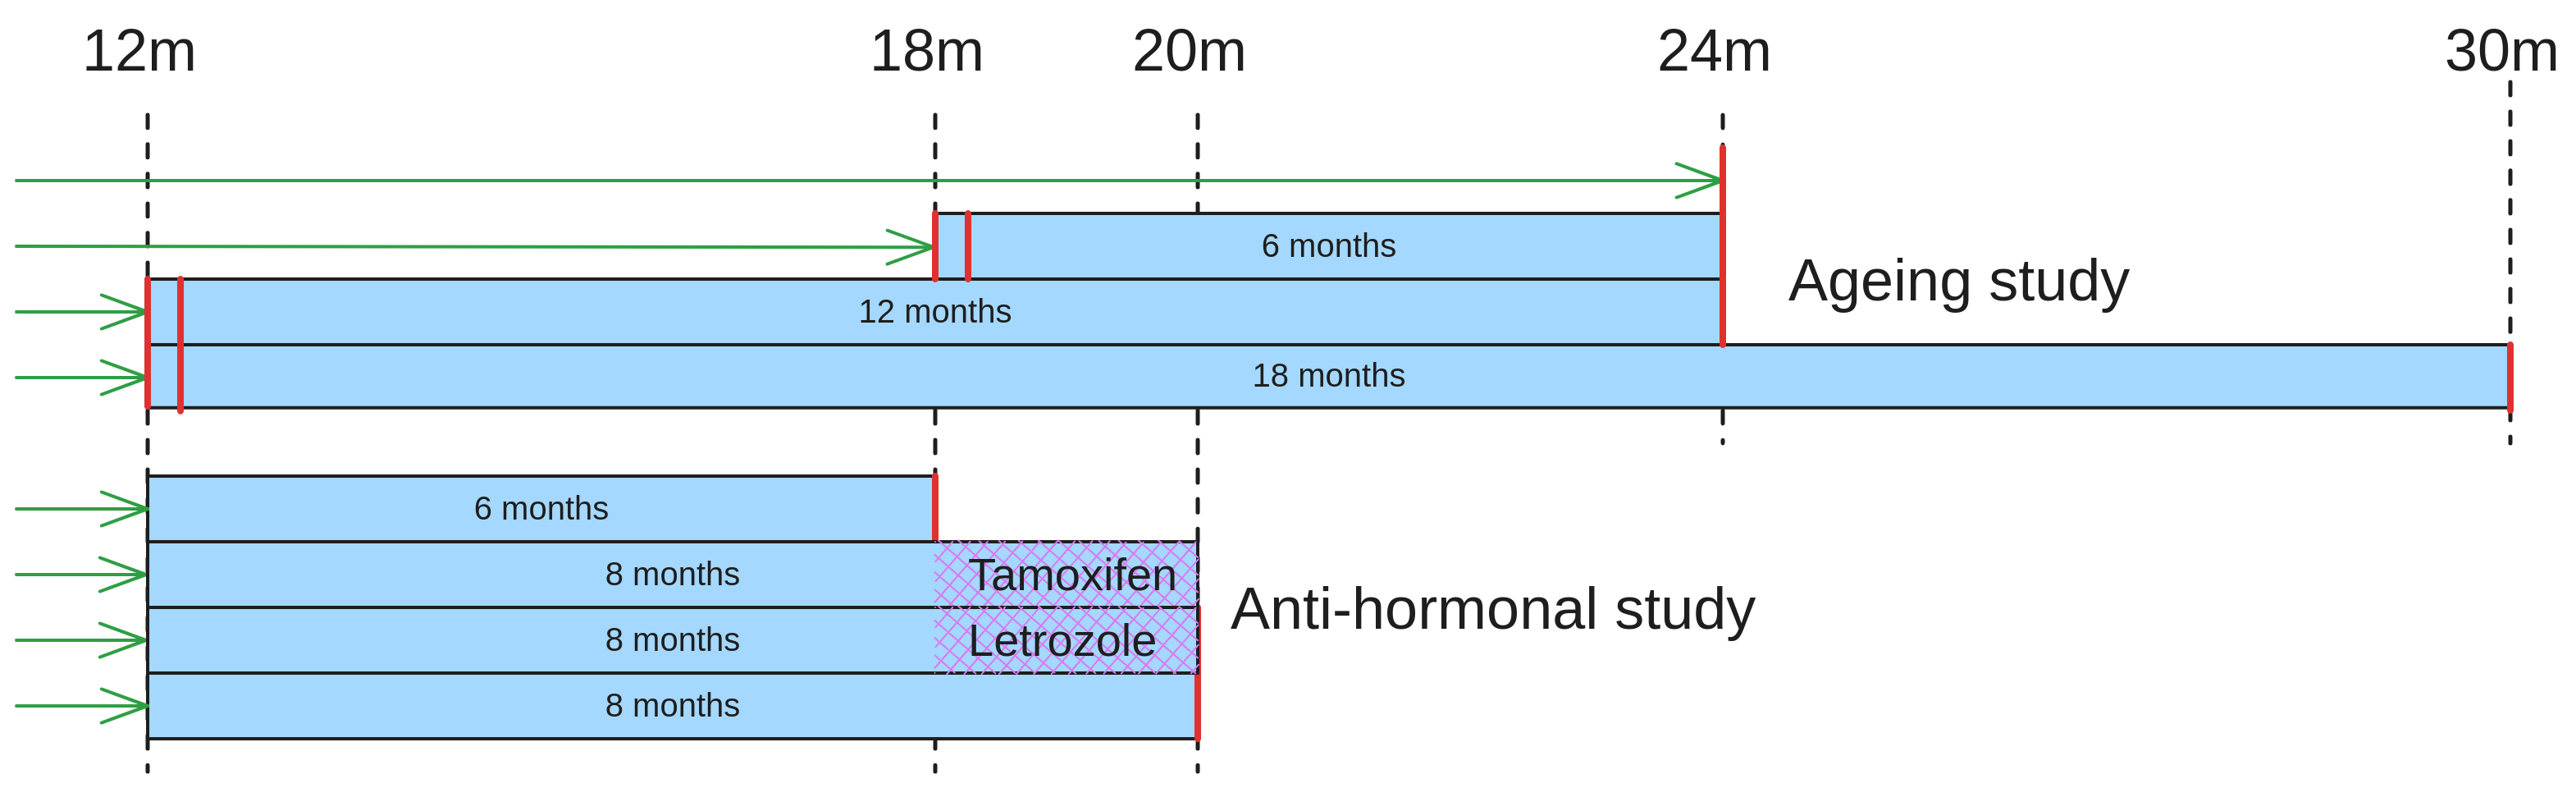
\includegraphics[width=\textwidth]{chapters/3_materials_and_methods/figures/datasets.png}
    \caption{Overview of the two studies and their respective timelines.
        Each red line represents two cohorts of mice that was euthanized for tissue
        collection: one with the \gls{esr1} transgene and one with the \gls{cyp19}
        transgene.
        The green arrows indicate periods without transgene induction, while the blue
        blocks indicate the periods of doxycycline treatment to induce the transgenes.
    } \label{fig:dataset_timeline} \end{figure}

\subsubsection{Differences in treatment}
The key difference between the two studies lies in the timing and duration of
the transgene induction, as well as the subsequent treatment with anti-hormonal
therapies.

\paragraph{Anti-hormonal study}
In the anti-hormonal study, eight different cohorts of mice were investigated,
four with the \gls{esr1} transgene and four with the \gls{cyp19} transgene.
As shown in \cref{fig:dataset_timeline}, the mice were treated with doxycycline
to induce the transgenes at 12 months of age, corresponding to middle age in
humans.

At 18 months of age (6 months of transgene induction), one cohort of each
genotype was euthanized to collect mammary gland tissue as a pre-treatment
control.
At the same time, two cohorts of each genotype were started being treated with
\gls{tam} or \gls{let}, respectively.
The remaining cohort of each genotype was left untreated as a control.

After two more months (now 20 months of age), the remaining three cohorts
(\gls{tam}, \gls{let}, control) of each genotype were
euthanized\supercite{furth_esr1_2023}.

\paragraph{Aging study}
The aging study consists of 16 cohorts of mice, eight with the \gls{esr1}
transgene and eight with the \gls{cyp19} transgene.
At 12 months of age, one cohort of each genotype was euthanized to collect
mammary gland tissue as a pre-transgene induction control.
For three cohorts of each genotype, the transgene induction was started at 12
months of age.

One of the three cohorts with transgene induction started at 12 months was
euthanized after 1 week of doxycycline treatment to assess the immediate
effects of the transgene induction.
The remaining two cohorts were euthanized at 24 and 30 months of age to
investigate the long-term effects of the transgene induction.

One cohort of each genotype that did not receive the transgene induction was
euthanized at 18 months of age.
Two other cohorts of each genotype started the transgene induction at 18 months
of age.
Of these two cohorts, one was euthanized after 1 week of doxycycline treatment,
while the other was euthanized at 24 months of age.

Lastly, one cohort of each genotype that did not receive any transgene
induction was euthanized at 24 months of
age\supercite{furth_overexpression_2023}.

\subsubsection{Sequencing process} \label{sec:dataset_sequencing}
Both studies used \gls{rna-seq} to analyze gene expression in the mammary
glands.
After euthanasia, thoracic mammary glands were flash frozen, and \gls{rna} was
extracted using a Direct Zol \gls{rna} miniprep kit.
The sequencing libraries were prepared from ribosome-depleted \gls{rna} and
sequenced using the Illumina NextSeq 550 platform with a single-end 75-bp read
length\supercite{furth_esr1_2023,furth_overexpression_2023}.

\subsubsection{Findings}

\paragraph{Anti-hormonal study}
The study found that \gls{esr1} overexpression significantly increased the
expression of genes related to cell proliferation, particularly those linked to
poor prognostic indicators in early-stage \gls{hr+} breast cancer.
\Gls{tam} and \gls{let} treatments were able to reduce this elevated
proliferative signature, but only \gls{esr1} mice showed substantial
responsiveness to \gls{tam} during reproductive senescence.
Both models were responsive to \gls{let} before and after reproductive
senescence\supercite{furth_esr1_2023}.

\paragraph{Aging study}
This study demonstrated that \gls{esr1} overexpression in aged mice led to a
higher prevalence of \gls{er+} mammary adenocarcinomas.
The tumors in \gls{esr1}-overexpressing mice were predominantly \gls{er+},
whereas \gls{cyp19} mice exhibited a mix of \gls{er+} and adenosquamous
carcinomas.
The \gls{esr1} mice developed a persistent proliferative signature similar to
that found in human \gls{er+} breast cancer, supporting the role of aging and
prolonged estrogen exposure in the generation of these
cancers\supercite{furth_overexpression_2023}.

\subsection{\Glsfmtshort{mirna} data}
\label{sec:mirna_data}

As explained in \cref{sec:circrna_functions}, \gls{mirna} sponging is one of
the most well-known functions of \glspl{crna}.
Unfortunately, the datasets described in \cref{sec:datasets} do not include
\gls{mirna} data - thus, it is not possible to identify \glspl{mirna} that were
actually present in the mice.

The closest alternative is using information from other studies that
investigated the \gls{mirna} expression in the same tissue and under similar
conditions.
For this purpose, I found a study by \textcite{wang_dynamic_2022} that
investigates how \glspl{mirna} are involved in regulating milk protein gene
expression during different stages of mammary gland development in mice.
The following paragraphs provide an overview of the study design and the main
findings.

\subsubsection{Study design}
The study collected mammary gland tissues from 15 specific-pathogen-free (SPF)
female ICR mice across five developmental stages: virgin, day 16 of pregnancy,
day 12 of lactation, and days 1 and 3 of forced weaning.
Tissues were frozen for RNA extraction, and small \glspl{rna} ranging from 18
to 30 nucleotides were isolated.
Adapter ligation and cDNA synthesis were performed, followed by amplification
for sequencing.
Using the DNBseq platform, approximately 21 million clean reads were generated
per sample.
After filtering low-quality reads, the clean reads were mapped to the mouse
genome with Bowtie2, identifying known \glspl{mirna} from existing databases,
while novel \glspl{mirna} were predicted using miRDeep2.
These miRNAs were grouped into 12 clusters based on expression profiles across
the developmental stages using the Mfuzz R package, revealing stage-specific
patterns.
Validation of the sequencing data was performed by qPCR on eight randomly
selected \glspl{mirna}, with strong correlation to the sequencing results.
Target genes of the \glspl{mirna} were predicted using TargetScan, miRanda, and
RNAhybrid, and functional analysis through \gls{go} and \gls{kegg} pathway
analysis revealed their involvement in mammary gland development and
lactation\supercite{wang_dynamic_2022}.

\subsubsection{Findings}
The study uncovered several key findings regarding the role of \glspl{mirna} in
regulating mammary gland development and milk protein expression in mice.
Researchers identified a total of 852 known \glspl{mirna} and 179 novel
\glspl{mirna} in the mammary glands across five investigated developmental
stages.
These \glspl{mirna} were grouped into 12 clusters based on their expression
patterns, with Cluster 1 \glspl{mirna} showing an inverse relationship with
milk protein gene expression.
Notably, the study identified a novel \gls{mirna}, mmu-miR424-5p, which was
found to regulate the expression of CSN2 (\textbeta{}-casein), a key milk
protein gene, indicating its role as a potential negative regulator of milk
protein synthesis\supercite{wang_dynamic_2022}.

The functional analysis of these \glspl{mirna} revealed that their target genes
were involved in crucial biological processes related to mammary gland
development, such as cell proliferation, differentiation, apoptosis, and lipid
metabolism.
Pathway analyses (\gls{go} and \gls{kegg}) further linked these \glspl{mirna}
to important signaling pathways, including the Wnt, mTOR, and MAPK pathways,
which are known to regulate mammary gland growth, differentiation, and milk
production\supercite{wang_dynamic_2022}.

\section{Nextflow and nf-core}
\label{sec:nextflow_and_nf-core}
\paragraph{Nextflow} is a workflow management system that enables the
development of reproducible and scalable workflows.
It allows the creation of complex pipelines that can be executed on a variety
of platforms, from local machines to cloud computing environments.
Nextflow uses a \gls{dsl} that simplifies the definition of workflows and
enables the reuse of existing components \supercite{di_tommaso_nextflow_2017}.
As a result, Nextflow has become a popular tool in the bioinformatics
community.

\begin{figure}[ht]
    \centering

    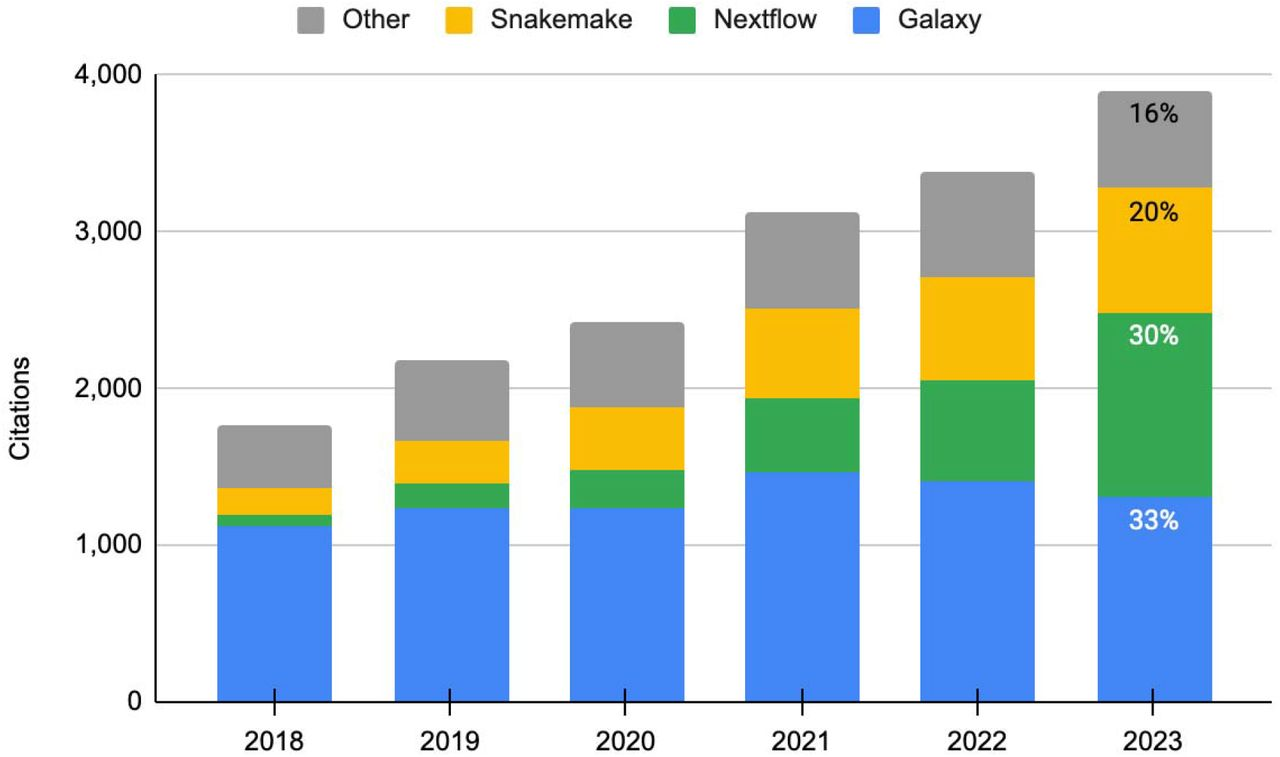
\includegraphics[width=\textwidth]{chapters/3_materials_and_methods/figures/nextflow_usage.jpg}
    \caption{Yearly citations of the most popular workflow management systems
        in bioinformatics.}
    \label{fig:nextflow_usage}
\end{figure}

As pointed out by Langer et al.
in a recent preprint
\supercite{langer_empowering_2024}, programming-based workflow systems like
Nextflow and Snakemake have gained popularity during the last years, while
GUI-based systems like Galaxy have lost ground.
Furthermore, Nextflow has been the fastest growing workflow system in the last
years, with a remarkable 30 percent share of citations in 2023
(\cref{fig:nextflow_usage}).
The authors mostly attribute this to the great quality of the pipelines curated
by the nf-core community
\supercite{langer_empowering_2024,grayson_automatic_2023}.

\paragraph{nf-core} is a community-driven project that provides a collection of
high-quality, reproducible, and scalable Nextflow pipelines.
These pipelines cover a wide range of bioinformatics applications, from
\gls{rna-seq} and \gls{chip-seq} to \gls{scrna-seq} and metagenomics
\supercite{ewels_nf-core_2020}.
The community maintains a collection of reusable components, so that developers
can utilize them to speed up the development of new pipelines.
The nf-core project also provides guidelines for best practices in pipeline
development, ensuring that the resulting workflows are robust, efficient, and
easy to use \supercite{ewels_nf-core_2020}.

\section{nf-core/circrna}
\label{sec:nf-core_circrna}
The nf-core/circrna pipeline has originally been published by Digby et al.
in
2023 \supercite{digby_nf-corecircrna_2023}.
Since then, the pipeline has gone through several updates and improvements.
The pipeline can utilize seven different tools for \gls{bsj} detection,
including CIRIquant, CIRCexplorer2, \gls{crna} finder, DCC, find\_circ,
MapSplice, and Segemehl.
It then annotates the detected \glspl{crna} using GTF-based and database-based
annotation.
The pipeline also extracts the sequences of the \glspl{crna} and quantifies
their expression levels together with the linear transcripts.
Finally, the pipeline performs \gls{mirna} interaction analysis using miRanda
and TargetScan, and provides several downstream analyses through a Shiny
application.
An overview of the pipeline is shown in \cref{fig:circrna_pipeline}.

\begin{figure}[ht]
    \centering

    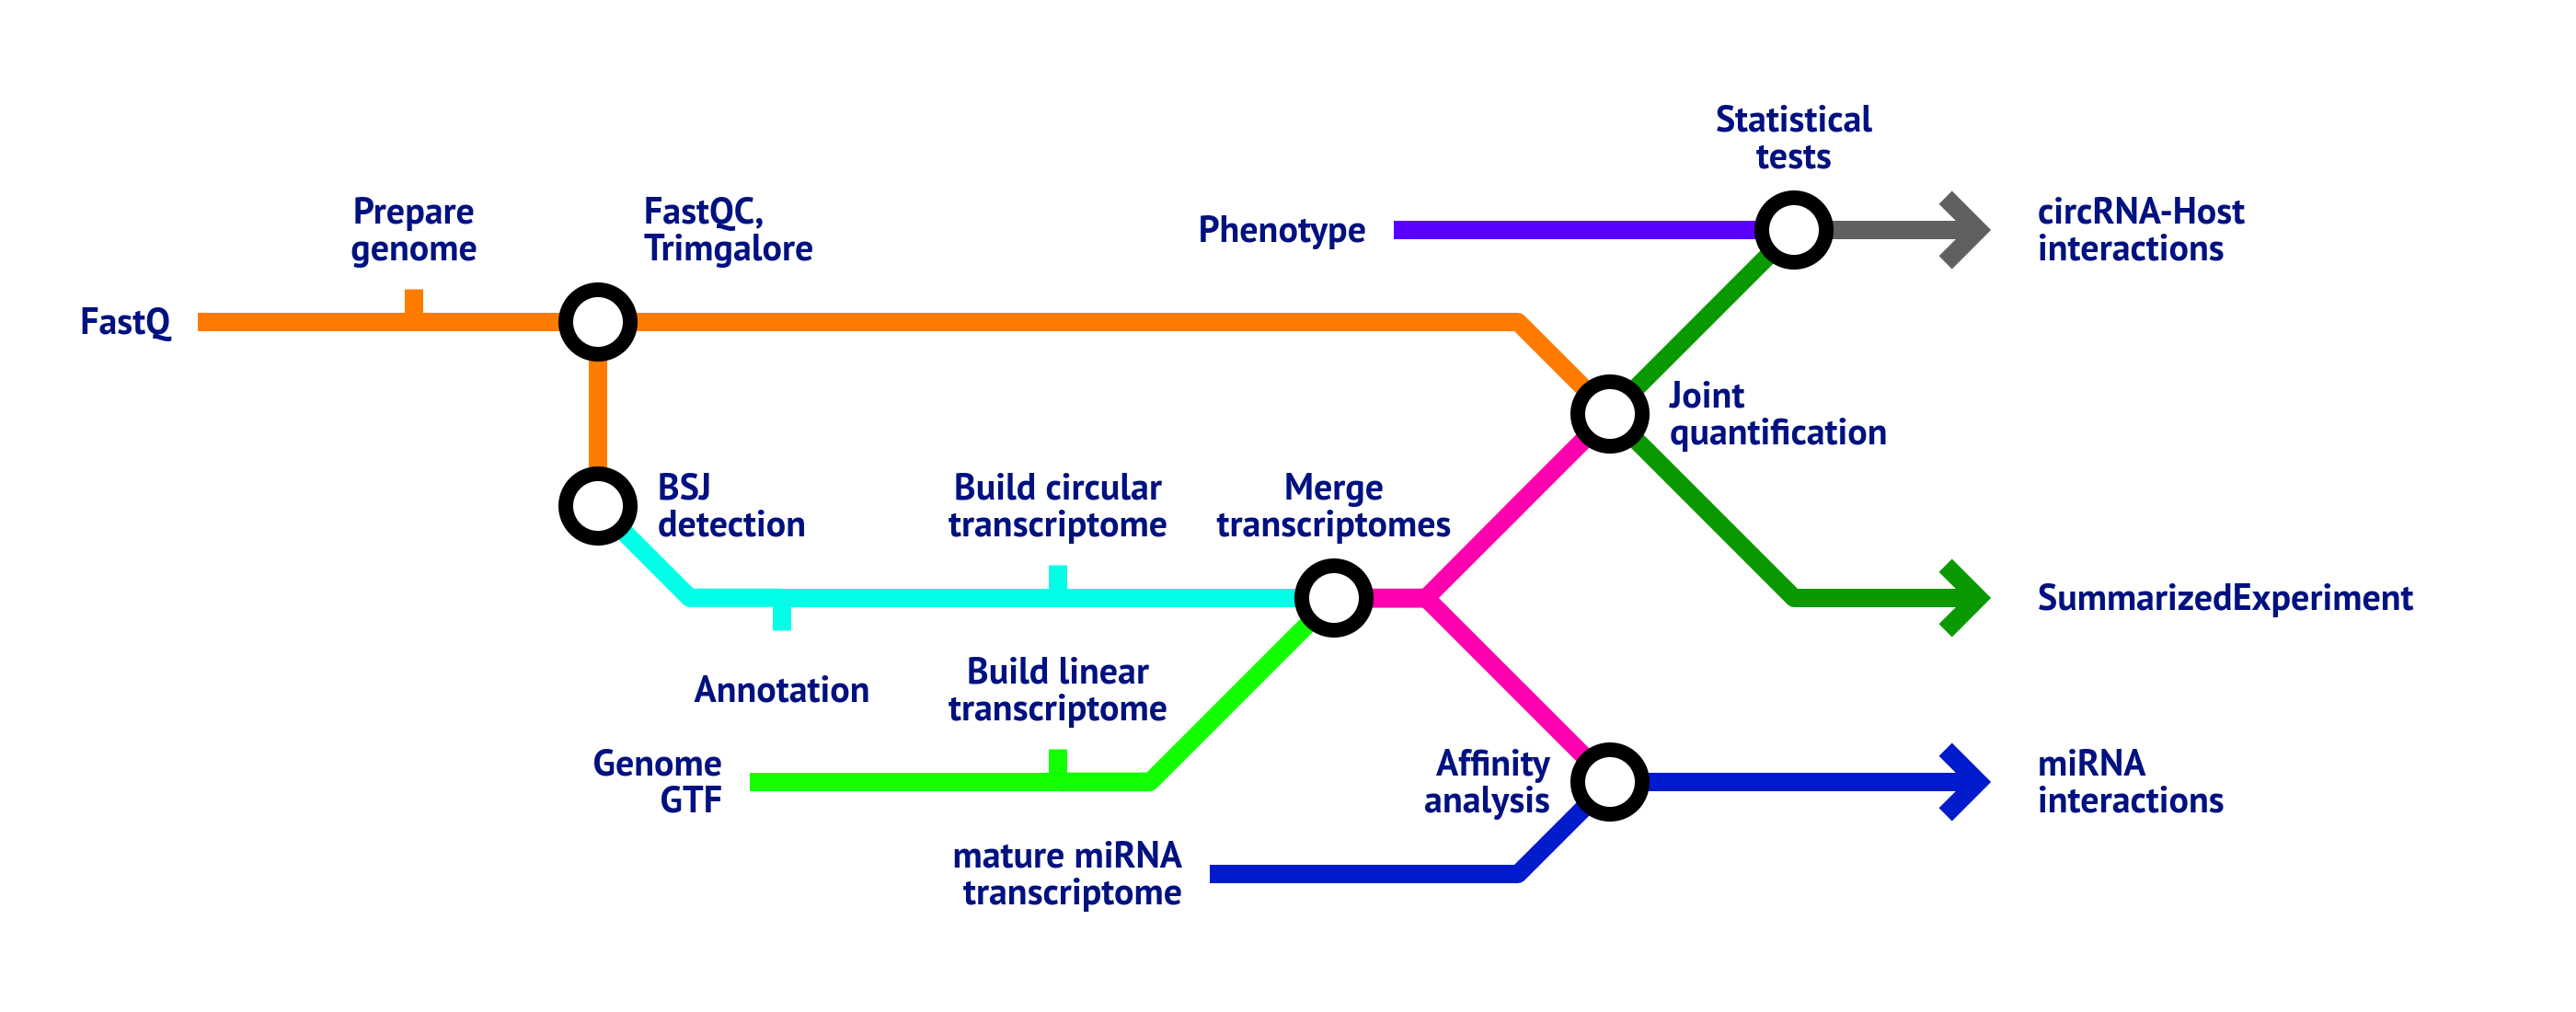
\includegraphics[width=\textwidth]{chapters/3_materials_and_methods/figures/nf-core_circrna.png}
    \caption{nf-core/circrna} % TODO: Add detailed caption
    \label{fig:circrna_pipeline}
\end{figure}

\subsection{\gls{crna} detection}
\label{subsec:circrna_detection}
From a molecular perspective, \gls{crna}s are similar to their linear
counterparts, with the primary distinction being their circular structure.
As explained in \cref{sec:circrna_biogenesis}, \gls{crna}s are derived from a
linear precursor (identical to linear RNA) that undergoes back-splicing to form
a loop.
Thus, the only way to computationally identify \gls{crna}s is by detecting
reads spanning the \gls{bsj}, which cannot be accounted for by canonical
forward splicing.
nf-core/circrna provides a total of seven tools for \gls{bsj}
detection.
However, only five of them are compatible with single-end sequencing data.
I will briefly discuss these five tools below.

\subsubsection{find\_circ (2013)}
Find\_circ is one of the pioneering tools for \gls{crna} detection,
specifically designed for identifying circular RNAs by leveraging RNA-seq data.
It employs a novel alignment strategy, splitting reads that do not map linearly
to the genome into smaller fragments, which are then re-aligned to detect
\gls{bsj}s\supercite{memczak_circular_2013}.
This tool does not rely on any known annotations and processes RNA-seq reads
using Bowtie, an efficient aligner for identifying \gls{bsj} reads.
One of its key features is that it filters for \gls{bsj} reads, removing those
that align entirely to the genome, which makes it stand out from methods
relying heavily on gene annotations\supercite{memczak_circular_2013}.

While it has been effective in many studies, it may not capture \gls{crna}s
with non-canonical splice signals, which can limit its detection
capabilities\supercite{sekar_circular_2018,liu_prkra_2022}.
Nonetheless, find\_circ remains a popular choice for researchers due to its
ease of use and integration with RNA-seq workflows.

\subsubsection{Segemehl (2014)}
Segemehl integrates a sensitive and flexible read-matching algorithm based on
enhanced suffix arrays (ESAs).
It identifies \gls{bsj} reads through split-read mapping, where the RNA-seq
data is aligned using a dynamic programming strategy that identifies splicing,
trans-splicing, and fusion transcripts.
Its major advantage over other tools is its ability to map reads containing
multiple split sites, which boosts sensitivity for detecting \gls{crna}s even
in complex cases like long reads or sequences with
errors\supercite{hoffmann_multi-split_2014}.

While Segemehl has shown promise in identifying \gls{crna}s, its performance
can vary depending on the specific dataset and experimental
conditions\supercite{gao_ciri_2015,zeng_comprehensive_2017}.

\subsubsection{DCC (2016)}
DCC relies on STAR as its underlying aligner, which maps RNA-seq reads to the
genome.
It uses a combination of filters to detect \gls{bsj}s by distinguishing
back-splice reads from linear splicing.
DCC integrates across replicates to minimize false positives and improve the
precision of \gls{crna} detection.
What sets DCC apart is its post-mapping step, where it not only detects
\gls{crna}s but also estimates their expression relative to the host gene using
read counts from junction and non-junction reads.
This makes it highly useful for comparing \gls{crna} expression across
conditions\supercite{cheng_specific_2016}.
DCC has been validated in numerous studies, demonstrating high reliability and
accuracy in \gls{crna} detection\supercite{paraboschi_interpreting_2018}.

\subsubsection{CIRCexplorer2 (2016)}
CIRCexplorer2 is another widely used tool that focuses on the detection of
\gls{crna}s by analyzing RNA-seq data.
It employs a unique strategy that combines both \gls{bsj} reads and linear RNA
reads to improve \gls{crna} identification.
CIRCexplorer2 has demonstrated robust performance in various studies, often
ranking high in comparative evaluations against other \gls{crna} detection
tools\supercite{zeng_comprehensive_2017,nicolet_circular_2018}.
Its ability to provide detailed annotations and quantifications of \gls{crna}s
makes it a valuable resource for researchers\supercite{hansen_comparison_2016}.
%TODO: Update

\subsubsection{CIRI2 (2018)}
CIRI2 improves upon the original CIRI\supercite{gao_ciri_2015} by using a
maximum likelihood estimation (MLE) based on multiple seed matching to detect
\gls{bsj} reads.
This algorithm is optimized for high sensitivity while maintaining a low false
discovery rate by filtering out false positives from repetitive sequences and
mapping errors.
It employs BWA-MEM for initial alignment, with CIRI2 distinguishing itself by
its efficient use of computational resources and ability to handle mixed read
lengths, making it faster and more memory-efficient compared to other
methods\supercite{gao_circular_2018}.

\subsection{\Glsfmtshort{crna} annotation}
In its minimal form, a \gls{crna} is defined by the chromosome it is located on
and the start and end position of the \gls{bsj}.
While this information is sufficient to uniquely identify a \gls{bsj}, it does
not provide any information about the gene or genes it is part of.
Furthermore, it does not give any information about the type of \gls{crna} it
is (types of \gls{crna} are described in \cref{sec:circrna_types}) and if it is
already has an entry in any \gls{crna} database.
While some tools like \gls{cex2} and \gls{dcc} provide their own annotation,
other tools like \gls{findcirc} and \gls{segemehl} do not.
To provide a consistent annotation for all \glspl{bsj}, \gls{nf-circrna} uses a
custom annotation process that will be described in the following sections.

\subsubsection{\gls{gtf}-based annotation}
\label{sec:gtf_annotation}
\gls{gtf} files are a common way to store genomic annotations like gene
locations and
transcript structures.
Such files are available for many reference genomes and can be used to identify
the genes and linear transcripts a \gls{crna} overlaps with.
This information can be used to infer the host gene(s) and the type of
\gls{crna}.

\begin{figure}[ht]
      \centering

      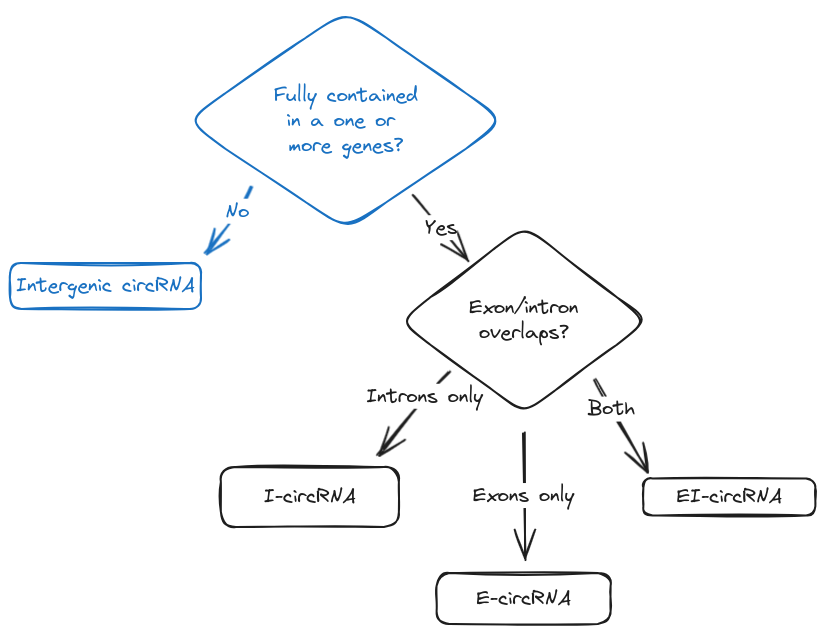
\includegraphics[width=\textwidth]{chapters/3_materials_and_methods/figures/annotation.png}
      \caption{Decision tree of the \gls{gtf}-based \gls{crna} type annotation}
      \label{fig:gtf_annotation}
\end{figure}

The \gls{nf-circrna} pipeline identifies the type of \gls{crna} as shown in
\cref{fig:gtf_annotation}: \begin{enumerate} \item If the \gls{crna} does not
            overlap with any gene, it is labeled as \gls{ig-crna}.
      \item If the \gls{crna} is fully contained in any gene, the following
            classification is performed:
            \begin{itemize}
                  \item If the \gls{crna} is fully contained in an exon, it is
                        labeled as \gls{e-crna}.
                  \item If the \gls{crna} is fully contained in an intron, it
                        is
                        labeled as \gls{i-crna}.
                  \item If the \gls{crna} spans both exonic and intronic
                        regions,
                        it is labeled as \gls{ei-crna}.
            \end{itemize}
\end{enumerate}

\subsubsection{Database-based annotation}
\label{sec:database_annotation}
In addition to \gls{gtf}-based annotation, \gls{nf-circrna} also provides
database-based annotation.
Databases like \gls{circbase} and \gls{circatlas} store information about known
\glspl{crna}, often including functional
information\supercite{glazar_circbase_2014,wu_circatlas_2023}.
Most \gls{crna} databases provide their stored \glspl{crna} in form of a
\gls{bed} file, providing a fairly unified interface for tools to process their
stored information in an automated fashion.
\gls{nf-circrna} allows the user to provide an arbitrary number of such
\gls{bed}
files for database-based annotation.
The pipeline identifies a match between a detected \gls{crna} and a database
entry, if the bi-directional overlap is at least 90\%.
This means that at least 90\% of the detected \gls{crna} must overlap with the
database entry and vice versa.

In this study, the following databases were used for annotation:

\paragraph{\Glsfmtlong{circbase}} \gls{circbase}, established in 2014, was one of the first
databases dedicated to \glspl{crna}.
It compiled data from nine large-scale studies, encompassing 92,375
\glspl{crna} from humans and key model
organisms\supercite{glazar_circbase_2014}.
Although \gls{circbase} was accessible at the beginning of this study, it has since
been taken offline.

\paragraph{\Glsfmtlong{circatlas}}
The latest version of \gls{circatlas} was released in early 2024 and offers a
more extensive dataset with three million vertebrate \glspl{crna}.
It covers ten species and 33 different tissues, providing valuable
cross-species conservation scores for researchers\supercite{wu_circatlas_2023}.

\subsection{\gls{crna} quantification}
\label{sec:crna_quantification}

While all \gls{bsj} detection tools quantify the number of reads
supporting each \gls{bsj}, there are several tools that focus on the
quantification of \glspl{crna} based on previously detected \glspl{bsj}.
nf-core/circrna offers two such tools: CIRIquant and
psirc-quant.

\subsubsection{CIRIquant}
\label{sec:ciriquant}
CIRIquant extends the CIRI (\Gls{crna} Identifier) framework, focusing on
accurate \gls{crna} quantification by re-aligning \gls{bsj} reads to a
pseudo-reference sequence.
Although it natively utilizes CIRI2 for \gls{bsj} detection, it can also
process \glspl{bsj} identified by other tools\supercite{zhang_accurate_2020}.
For each \gls{bsj}, CIRIquant constructs a pseudo \gls{crna} reference by
concatenating two copies of the sequence between the \gls{bsj} start and end
positions.
By comparing alignments to both the reference genome and the pseudo-reference
sequence, CIRIquant calculates the fraction of reads utilizing the \gls{bsj}
among those that span at least one of its
boundaries\supercite{zhang_accurate_2020}.
The output provided by CIRIquant is essentially the CPM (counts per million) of
reads supporting each \gls{bsj}, normalized by the total number of mapped reads
in the sample.

\subsubsection{psirc}
\label{sec:psirc}
As illustrated in \cref{fig:psirc_workflow}, psirc operates in two main phases:
first, the identification of \gls{bsj} and inference of full-length isoforms
(FLI); and second, the quantification of expression levels for the detected
isoforms\supercite{yu_quantifying_2021}.

\begin{figure}[ht] \centering

    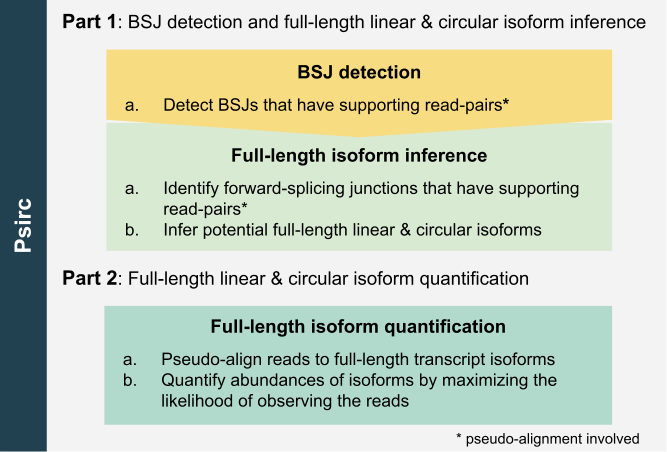
\includegraphics[width=0.5\textwidth]{chapters/3_materials_and_methods/figures/psirc_pipeline.png}
    \caption{psirc-workflow} \label{fig:psirc_workflow} \end{figure}

The initial phase of the workflow functions similarly to the implementation
described in \cref{sec:ciriquant}, with the added step of full-length isoform
inference.
However, this step requires paired-end sequencing data, which is not available
in this thesis.
While psirc's \gls{bsj} detection can be substituted with other tools, the FLI
inference step is more challenging to replace.
Previous studies have attempted to address this by using information from the
linear transcriptome to retain only exonic regions within the \gls{bsj} limits
\supercite{hoffmann_circrna-sponging_2023}.
If no exonic regions are present, the entire sequence is retained.
In contrast, the nf-core/circrna pipeline takes a different approach, retaining
the entire sequence within the \gls{bsj} boundaries, regardless of exonic
region presence.
This method avoids assumptions about the internal structure of the \gls{crna}.

For the quantification phase, psirc requires a combined transcriptome FASTA
file containing both linear and circular transcripts.
Psirc constructs a Transcript de Bruijn Graph (T-DBG) from this combined
transcriptome and utilizes Kallisto to jointly quantify the expression levels
of both transcript types\supercite{yu_quantifying_2021}.
This approach enables a direct comparison between linear and circular isoforms,
potentially offering deeper insights into the regulatory roles of \glspl{crna}
in gene expression.
Notably, psirc does not explicitly differentiate between reads spanning the
\gls{bsj} and those fully contained within it; instead, it relies on Kallisto's
likelihood maximization to distinguish between linear and circular
isoforms\supercite{yu_quantifying_2021}.

\subsection{\gls{mirna} interaction analysis}
The analysis of circular RNA (\gls{crna}) interactions with microRNAs (\gls{mirna}s)
is crucial for understanding the regulatory roles of \gls{crna}s in various
biological processes.
Two prominent tools used for predicting \gls{crna}-\gls{mirna} interactions are
MiRanda and TargetScan.
These tools leverage sequence complementarity and binding energy calculations
to identify potential \gls{mirna} binding sites within \gls{crna} sequences, thereby
elucidating their roles as competitive endogenous RNAs (ceRNAs).

\subsubsection{MiRanda}
MiRanda is a widely utilized algorithm that predicts \gls{mirna} targets based on
sequence complementarity and the stability of the RNA duplex formed between the
\gls{mirna} and its target.
It has been effectively employed in various studies to analyze \gls{crna}-\gls{mirna}
interactions.
For instance, Vromman et al.
noted that
MiRanda is often used alongside TargetScan to predict \gls{mirna} binding sites in
\gls{crna} sequences, contributing to a better understanding of \gls{crna}
functions
in gene regulation\supercite{vromman_closing_2021}.
Similarly, Zhang et al.
utilized
MiRanda in conjunction with TargetScan to predict microRNA response elements
(MREs) in differentially expressed \gls{crna}s, demonstrating its utility in
identifying significant interactions\supercite{zhang_microarray_2017}.

\subsubsection{TargetScan}
TargetScan, on the other hand, focuses on the identification of conserved \gls{mirna}
binding sites across species, which enhances the reliability of the predicted
interactions.
This tool has been integrated into various studies to explore the regulatory
networks involving \gls{crna}s and \gls{mirna}s.
For example, Jin et al.
employed MiRanda and TargetScan to predict interactions between \gls{crna}s and
\gls{mirna}s, reinforcing the hypothesis that \gls{crna}s can act as \gls{mirna}
sponges\supercite{jin_changes_2018}.
Furthermore, the combination of these tools allows researchers to construct
comprehensive \gls{crna}-\gls{mirna}-\gls{mrna} networks, elucidating the complex
regulatory mechanisms at play in various
diseases\supercite{he_construction_2021,zhang_construction_2021}.


\section{Downstream analyses}

\subsection{Differential expression analysis}

\subsubsection{DESeq2}

Many studies used aggregations of the counts of reads supporting a \gls{bsj}
from multiple detection tools followed by differential expression analysis
using traditional tools like DESeq2\supercite{love_moderated_2014} and
EdgeR\supercite{robinson_edger_2010}
\supercite{digby_nf-corecircrna_2023,gaffo_sensitive_2022}.

This approach has recently been improved by \textcite{buratin_detecting_2022},
who implemented a generalized linear mixed model approach which can handle the
count information from multiple detection tools, without the need for prior
aggregation\supercite{digby_computational_2024}.
However, this approach is not yet implemented as an easy-to-use tool and was
thus not used in this study.

\subsubsection{CIRIquant}

While CIRIquant is primarily a quantification tool, it also provides a
differential expression analysis feature.
While it lacks the flexibility of DESeq2 (e.g., in terms of design matrix
specification and tests for association with numeric covariates), it was
specifically designed for \gls{crna} data.

\subsection{Functional enrichment analysis}

\subsubsection{ClusterProfiler}

\subsubsection{Gene Ontology}

\chapter{Results and Discussion}

From a molecular perspective, circRNAs are similar to their linear
counterparts, with the primary distinction being their circular structure.
As explained in \cref{sec:circrna_biogenesis}, circRNAs are derived from a
linear precursor (identical to linear RNA) that undergoes back-splicing to form
a loop.
Thus, the only way to computationally identify circRNAs is by detecting reads
spanning the back-splice junction (BSJ), which cannot be accounted for by
canonical forward splicing.
Several tools for BSJ detection are discussed in
\cref{subsec:circrna_detection}.

However, detecting BSJs only reveals the start and end positions of a circRNA
within the genome, without providing information on its internal structure.
To reconstruct the full circRNA sequence, a de novo assembly of the circular
transcriptome that accounts for back-splice junctions is necessary.
Tools like CIRI-full, circRNAfull, JCcirc, and psirc can achieve this, but they
rely on paired-end or long-read sequencing data.
As of now, no tools are available for de novo assembly of circRNAs using
single-end short-read data, to my knowledge.
Since the data used in this thesis is single-end, the focus will be limited to
the detection, quantification, and analysis of BSJs.

\section{\Acrfull{bsj} detection}

For detection of \gls{bsj}s, I used the five tools already introduced in
\cref{subsec:circrna_detection}.
As shown in \cref{fig:detection_bars}, find\_circ, CIRI2, DCC, and
circexplorer2 detect a similar number of \gls{bsj}s, while segemehl detects
almost ten times as many \gls{bsj}s as its closest competitor, DCC.

\begin{figure}[ht] \centering

    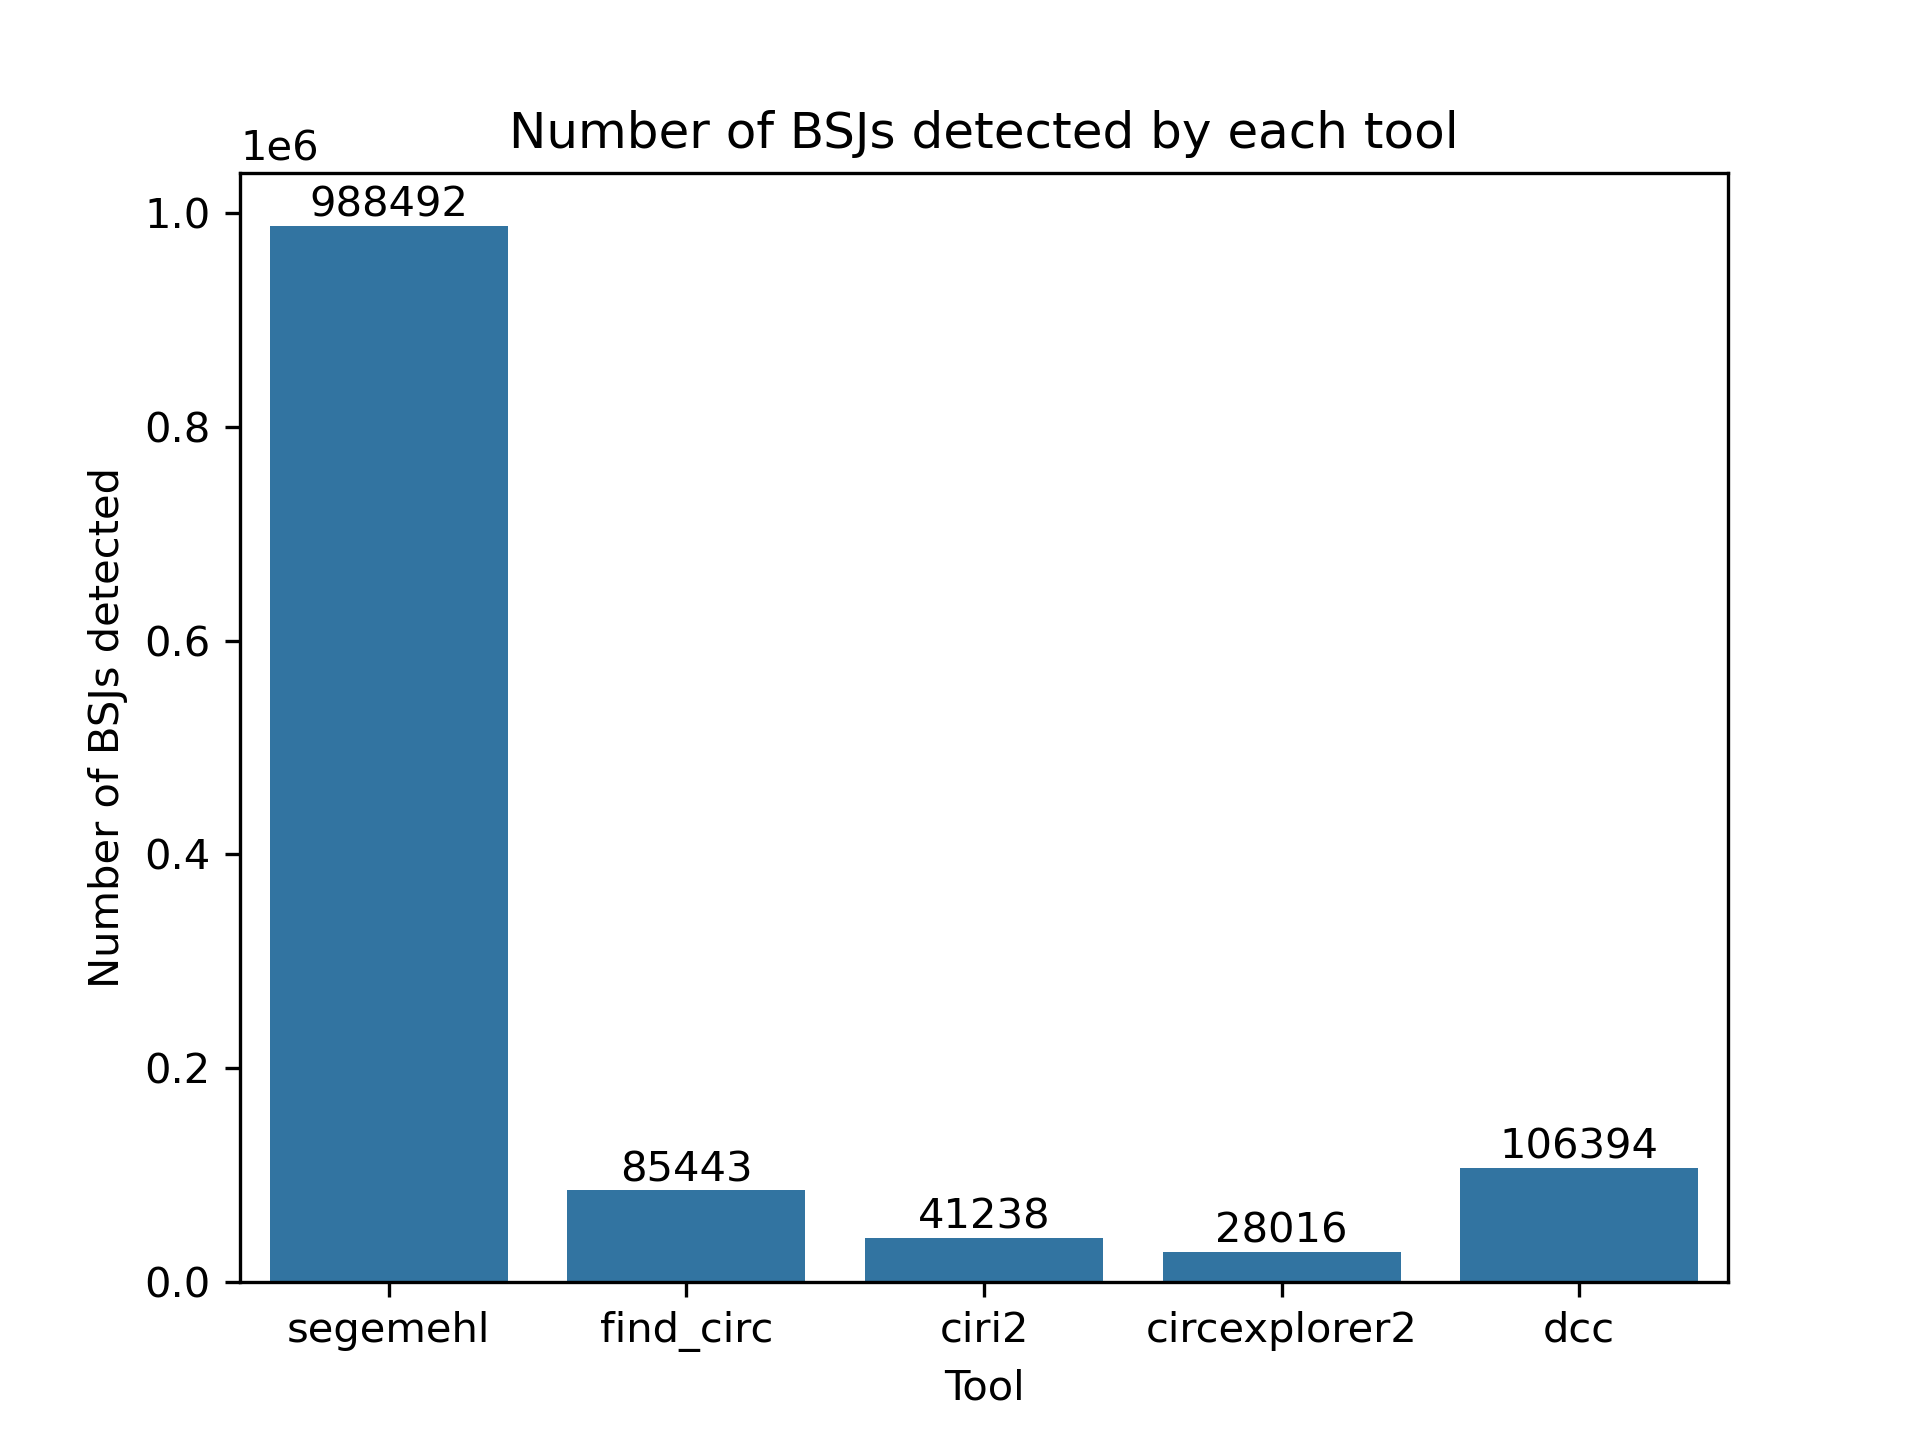
\includegraphics[width=0.7\textwidth]{chapters/4_results_and_discussion/figures/detection/n_bsjs_detected.png}
    \caption{Number of \gls{bsj}s detected by each tool.
        While find\_circ, CIRI2, DCC and circexplorer2 detect a similar number of
        \gls{bsj}s, segemehl detects a much larger number of \gls{bsj}s.
    }
    \label{fig:detection_bars}
\end{figure}
Similar behavior was previously observed by \textcite{zeng_comprehensive_2017},
where segemehl was among the top performers in terms of sensitivity, but also
had a high false positive rate.
The lowest numbers of \gls{bsj}s were detected by circexplorer2 and CIRI2,
which both have built-in filters to reduce false
positives\supercite{zhang_diverse_2016,gao_circular_2018}.

\subsection{Agreement between tools}

To assess the agreement between the tools, I used UpSet plots, which show the
overlap of \gls{bsj}s detected by different tools.
When identifying the overlap between tools, the most strict approach is to
consider only \gls{bsj}s with identical start and end positions and on the same
strand as the same \gls{bsj}.
The according plot is shown in \cref{fig:detection_upset_0_strand}.
While there are a total of x \gls{bsj}s detected by at least two tools, only y
\gls{bsj}s are detected by three tools, and none are detected by four or five
tools.

When ignoring the strand information, the number of \gls{bsj}s detected by
three tools increases substantially, as shown in
\cref{fig:detection_upset_0_nostrand}.
Also the number of \gls{bsj}s detected by two tools increases, while still no
\gls{bsj}s are detected by four or five tools.

Allowing a shift of 1 bp in the start and end positions while ignoring the
strand information changes the results drastically.
As shown in \cref{fig:detection_upset_1_nostrand}, a large number of \gls{bsj}s
are detected by four and even five tools.

As shown in \cref{fig:detection_upset_1_strand}, allowing a shift of 1 bp while
considering the strand information also leads to a number of \gls{bsj}s
detected by four and five tools, but the number is way lower than when ignoring
the strand information.

Increasing the allowed shift to larger values, e.g., 20 bp, does not lead to a
substantial change compared to the results when allowing a shift of 1 bp, as
shown in \cref{fig:detection_upset_20_nostrand}.

\begin{figure}[ht] \begin{tabular}{cc} \begin{subfigure}{.5\textwidth}
                                           \centering

                                           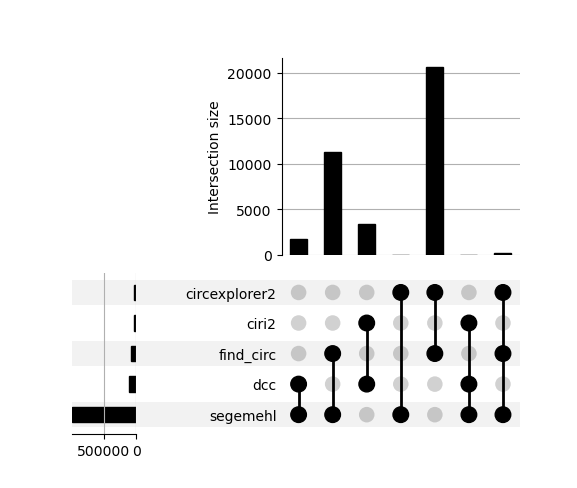
\includegraphics[width=\linewidth]{chapters/4_results_and_discussion/figures/detection/upset/diff_0_strand.png}
                                           \caption{No shift allowed, strand
                                               considered}
                                           \label{fig:detection_upset_0_strand}
                                       \end{subfigure} &
               \begin{subfigure}{.5\textwidth} \centering

                       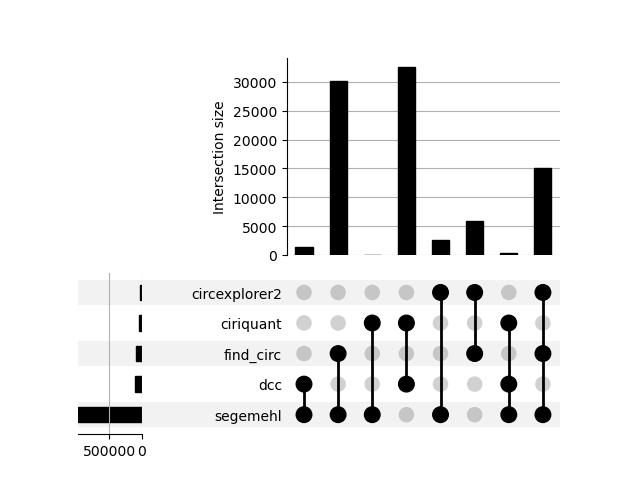
\includegraphics[width=\linewidth]{chapters/4_results_and_discussion/figures/detection/upset/diff_0_nostrand.png}
                       \caption{No shift allowed, strand ignored}
                       \label{fig:detection_upset_0_nostrand} \end{subfigure}
               \\ \multicolumn{2}{c}{
                   \begin{subfigure}{\textwidth} \centering

                           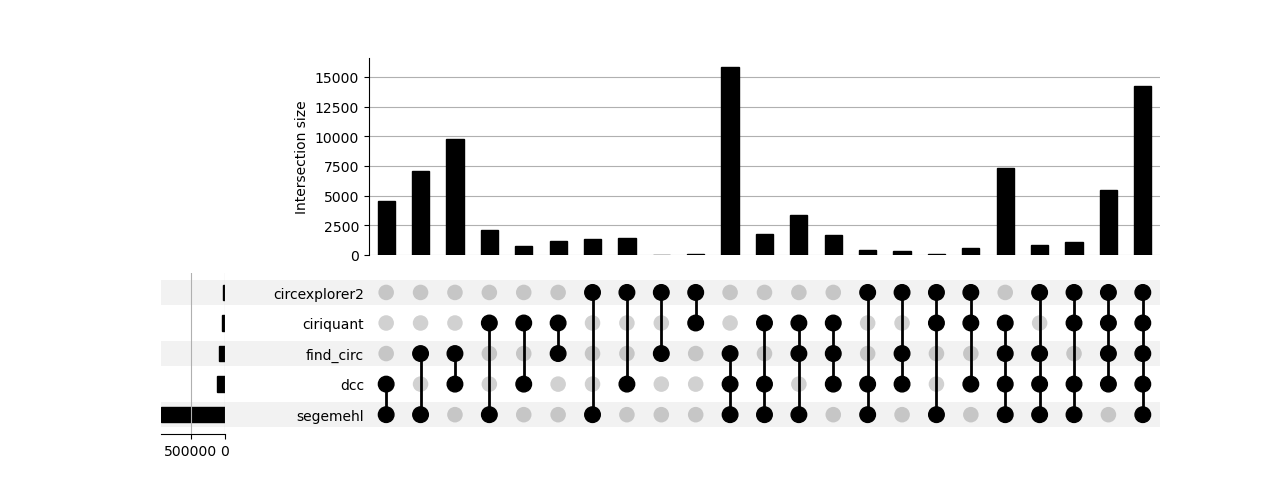
\includegraphics[width=\linewidth]{chapters/4_results_and_discussion/figures/detection/upset/diff_1_nostrand.png}
                           \caption{Shift of 1 allowed, strand ignored}
                           \label{fig:detection_upset_1_nostrand}

                       \end{subfigure}}\end{tabular} \caption{Upset plots
        showing the overlap of
        \gls{bsj}s detected by different tools using various grouping criteria.
        Only groups with at least two agreeing tools are displayed.
        When considering strand information and only counting \gls{bsj}s with identical
        start and end positions, many \gls{bsj}s are detected by just two tools, with
        very few detected by three tools (\cref{fig:detection_upset_0_strand}).
        Ignoring the strand information substantially increases the number of
        \gls{bsj}s detected by 3 tools (\cref{fig:detection_upset_0_nostrand}).
        Allowing a shift of 1 bp in the start and end positions while ignoring the
        strand information changes the results drastically, leading to a large number
        of \gls{crna}s with agreement between 4 and even 5 tools
        (\cref{fig:detection_upset_1_nostrand}).
    }
    \label{fig:detection_upset}
\end{figure}

\begin{figure}[ht]
    \centering

    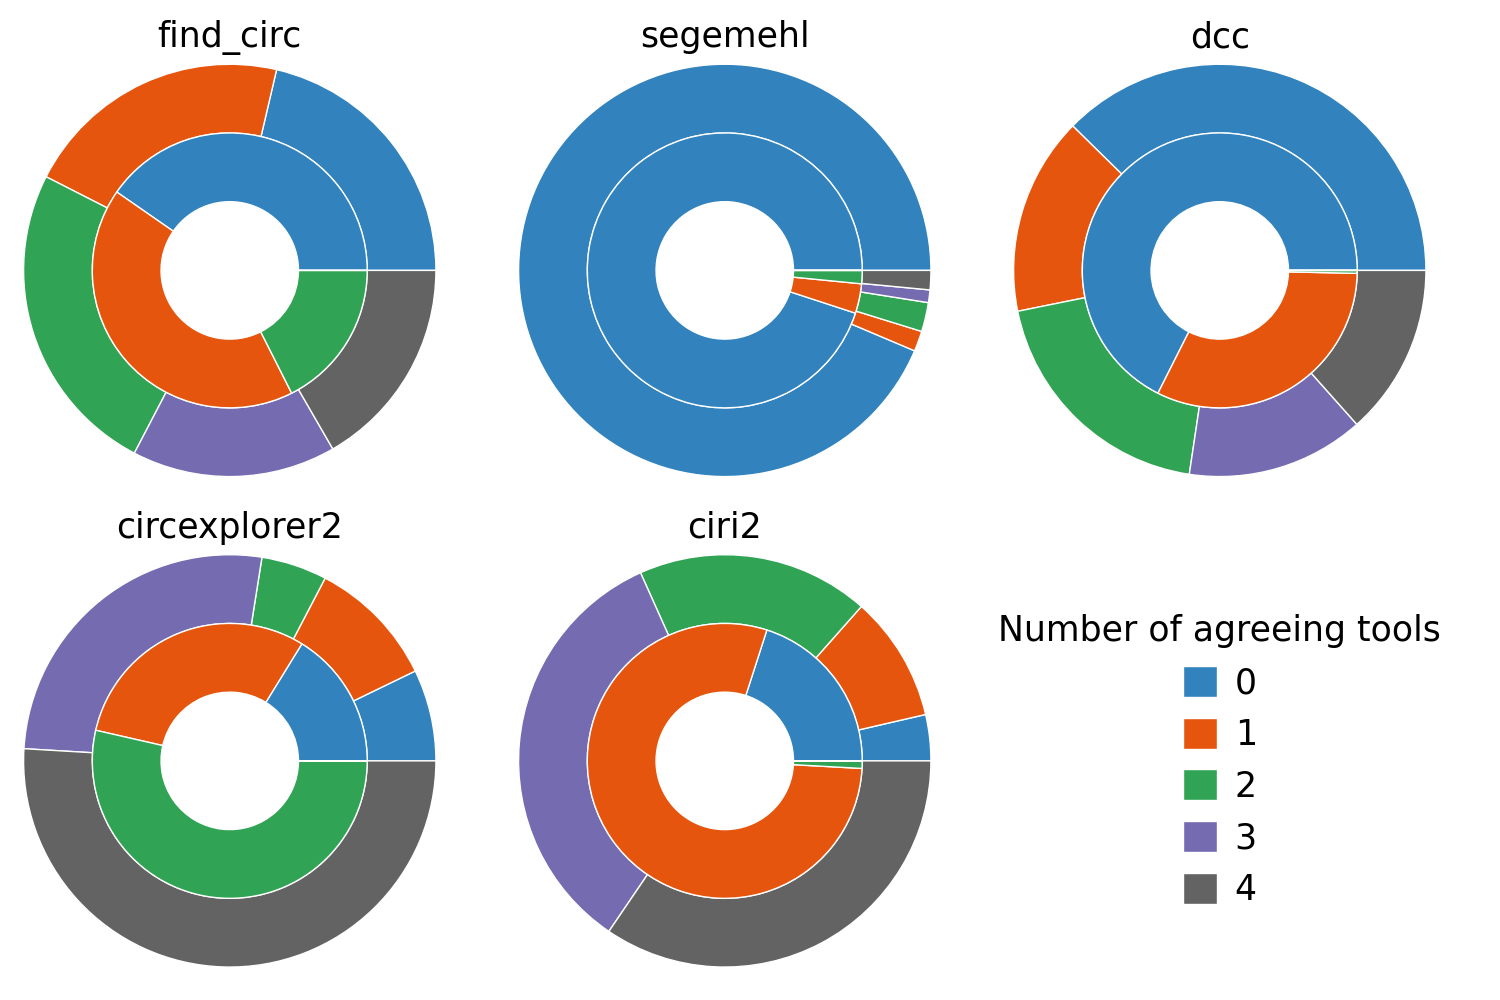
\includegraphics[width=0.7\textwidth]{chapters/4_results_and_discussion/figures/detection/pies.png}
    \caption{Pie charts showing the agreement of each tool with the others.
        The inner circle shows the agreement without allowing a shift in the start and
        end positions, while the outer circle shows the agreement when allowing a shift
        of 1 bp.
        While find\_circ, dcc, circexplorer2, and ciriquant behave similarly, segemehl
        detects a much larger number of \gls{bsj}s, with a large portion of them not
        being detected by any other tool.
    }
    \label{fig:detection_pies}
\end{figure}

\begin{figure}[ht]
    \begin{tabular}{cc}
        \begin{subfigure}{.4\textwidth}
            \centering

            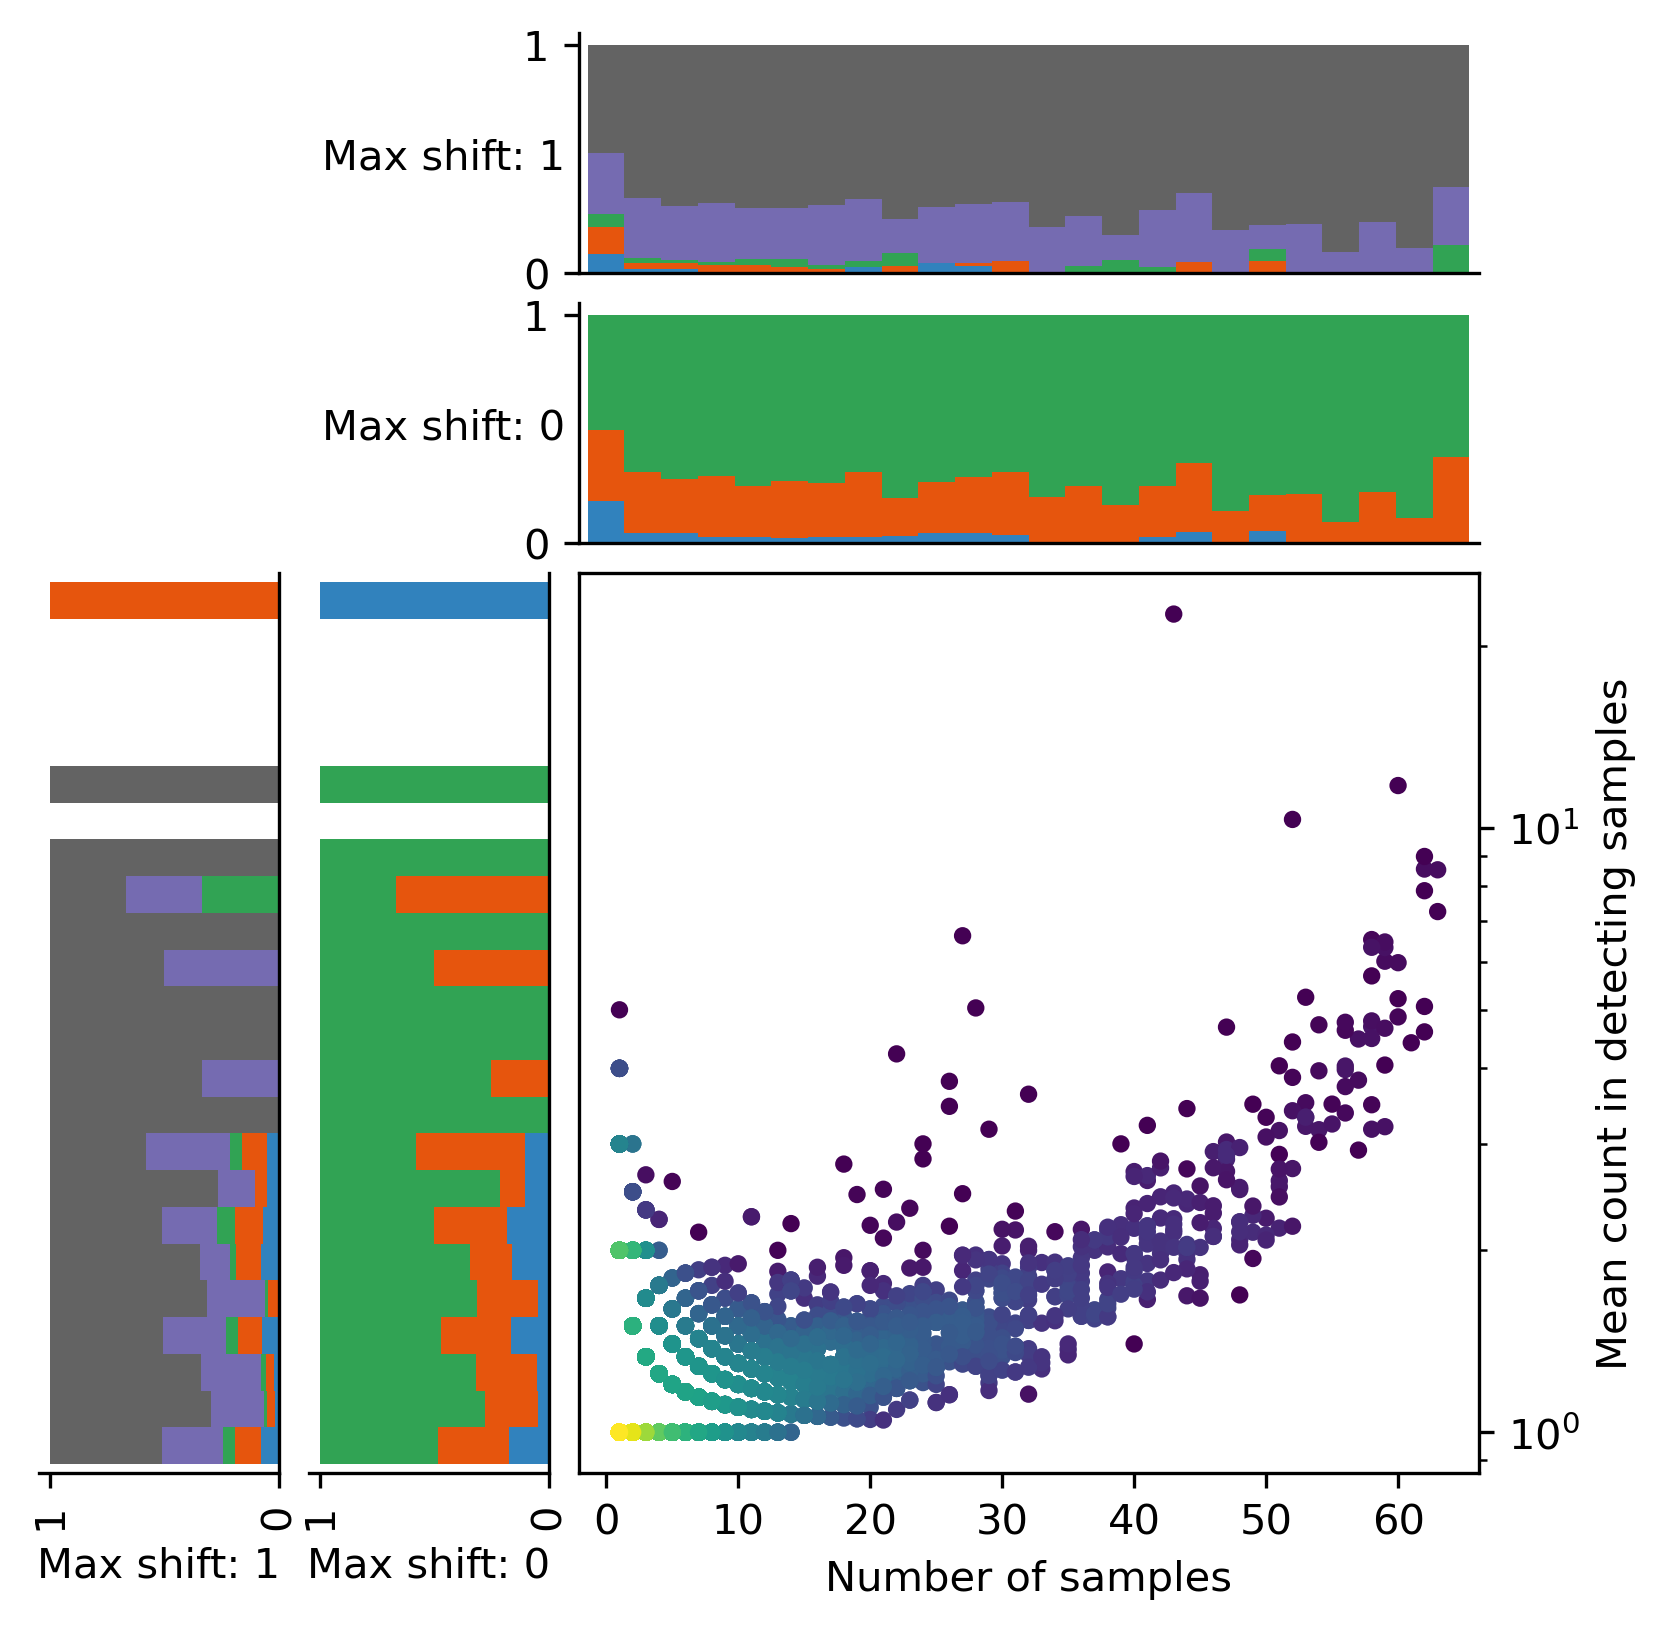
\includegraphics[width=\linewidth]{chapters/4_results_and_discussion/figures/detection/density/circexplorer2.png}
            \caption{CircExplorer2}
            \label{fig:detection_density_circexplorer2}
        \end{subfigure}
         &
        \begin{subfigure}{.4\textwidth}
            \centering

            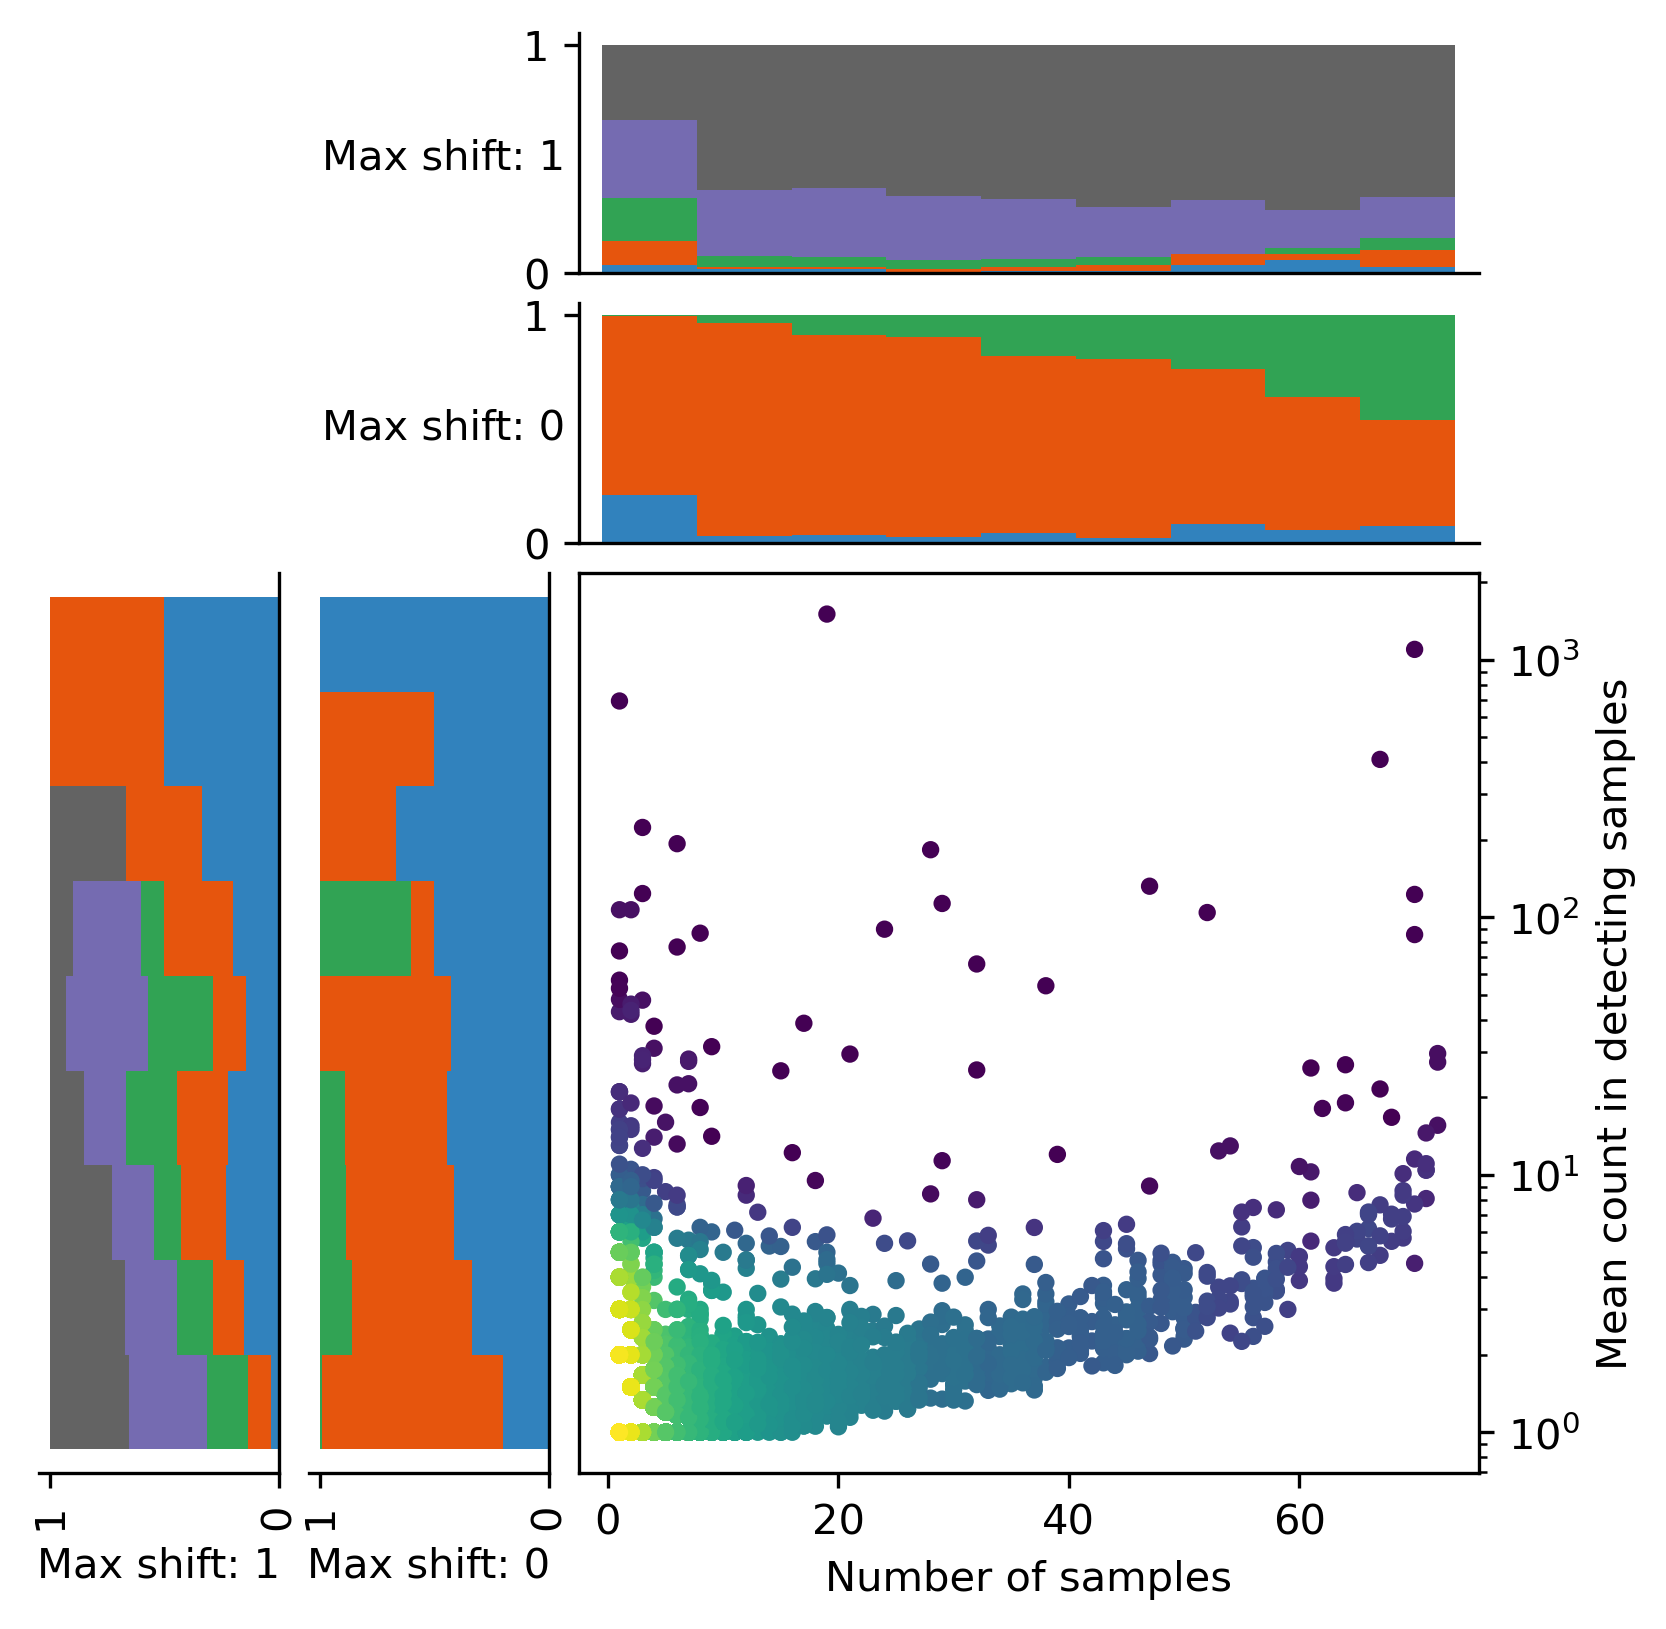
\includegraphics[width=\linewidth]{chapters/4_results_and_discussion/figures/detection/density/ciri2.png}
            \caption{CIRI2}
            \label{fig:detection_density_ciri2}
        \end{subfigure}     \\
        \begin{subfigure}{.4\textwidth}
            \centering

            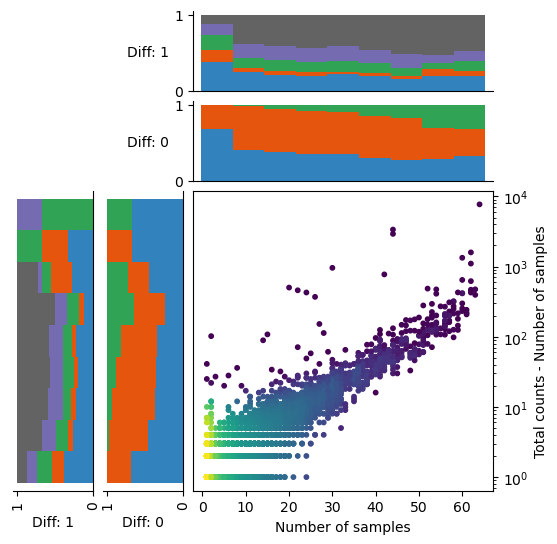
\includegraphics[width=\linewidth]{chapters/4_results_and_discussion/figures/detection/density/dcc.png}
            \caption{DCC}
            \label{fig:detection_density_dcc}
        \end{subfigure}
         &
        \begin{subfigure}{.4\textwidth}
            \centering

            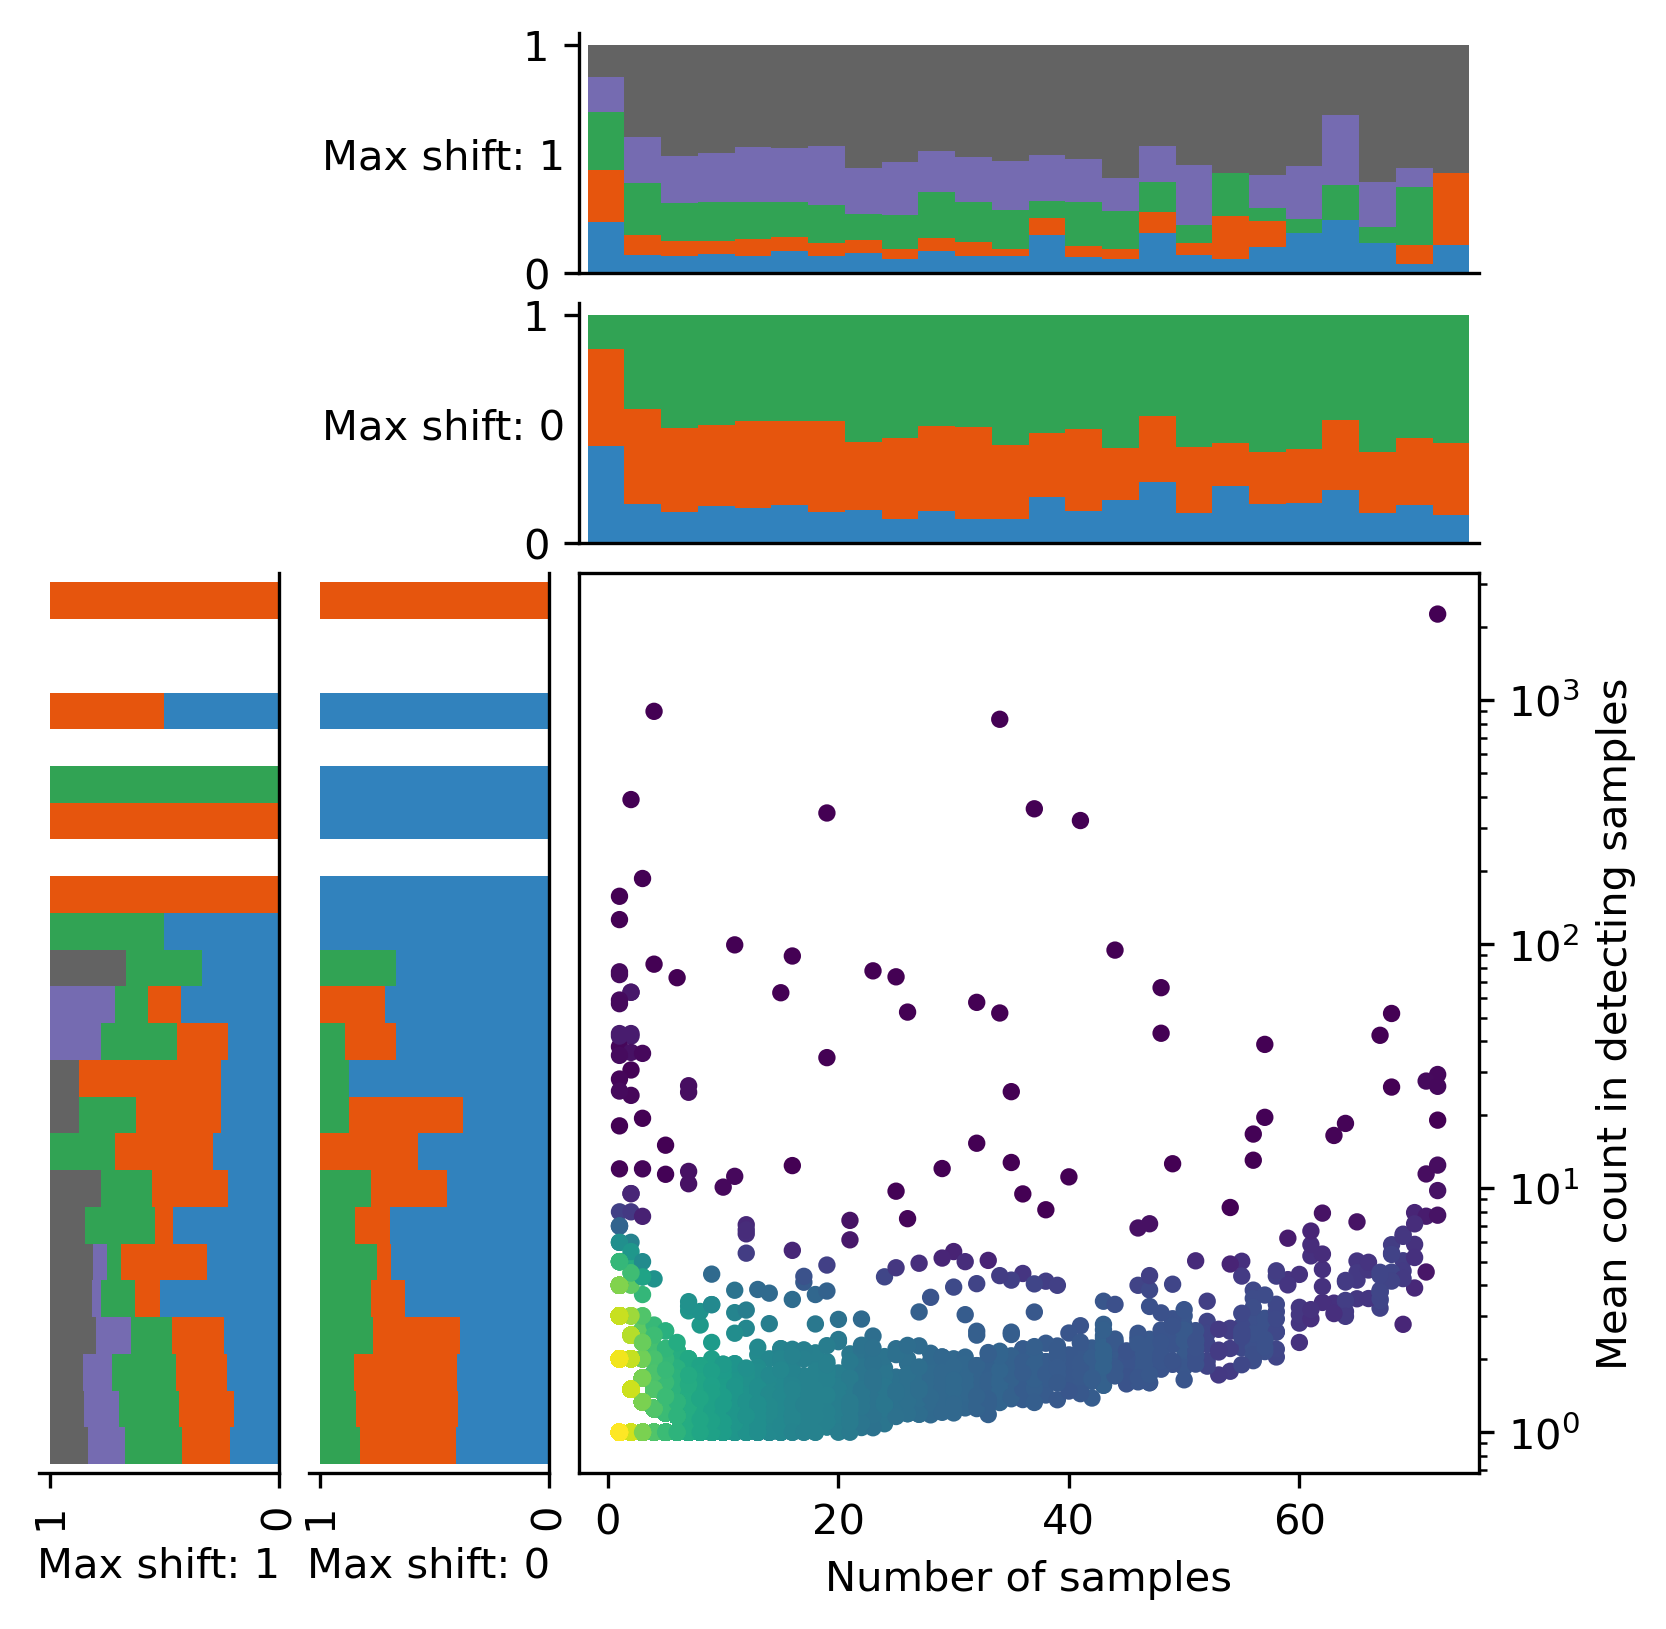
\includegraphics[width=\linewidth]{chapters/4_results_and_discussion/figures/detection/density/find_circ.png}
            \caption{find\_circ}
            \label{fig:detection_density_find-circ}
        \end{subfigure} \\
        \begin{subfigure}{.4\textwidth}
            \centering

            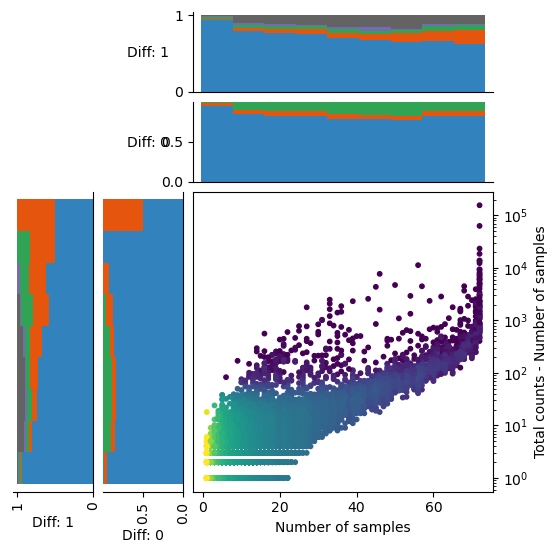
\includegraphics[width=\linewidth]{chapters/4_results_and_discussion/figures/detection/density/segemehl.png}
            \caption{Segemehl}
            \label{fig:detection_density_segemehl}
        \end{subfigure}
         &
        \begin{subfigure}{.4\textwidth}
            \centering
            % TODO: Add legend
            %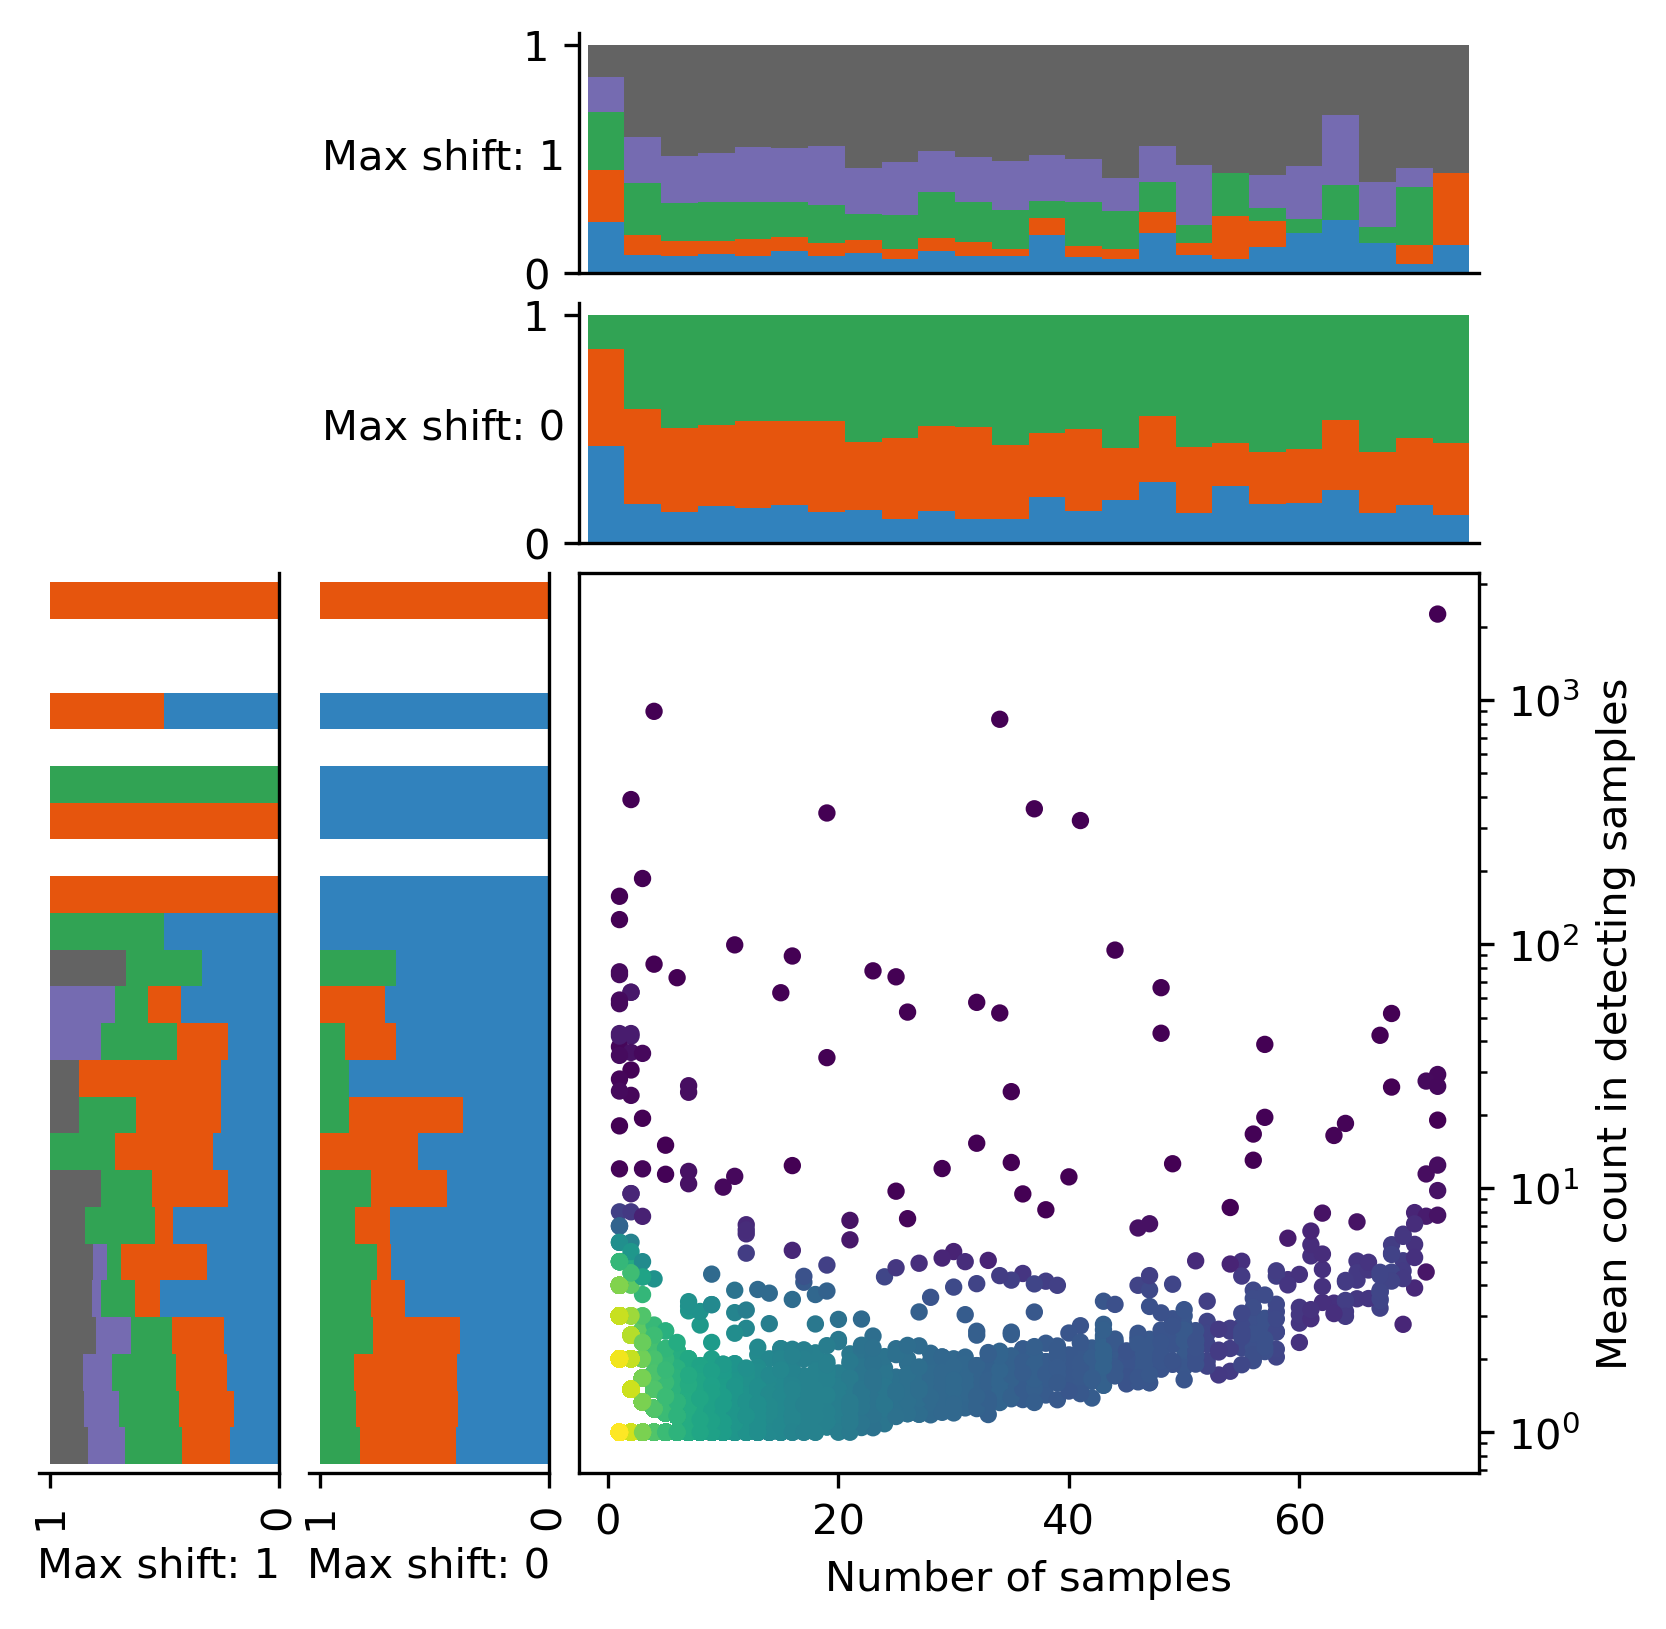
\includegraphics[width=\linewidth]{chapters/4_results_and_discussion/figures/detection/density/find_circ.png}
            \caption{Legend}
        \end{subfigure}
    \end{tabular}
    \caption{Distributions of \gls{bsj}s detected by each tool.
        The x-axis shows the number of tools that detected a \gls{bsj}, while the
        y-axis shows the logarithm of the number of reads supporting the \gls{bsj}
        across all samples.
        The color indicates the density of \gls{bsj}s at a given point.
        The stacked bar plots above and left of the scatter plots show the number of
        agreeing tools in the respective slice.
    }
    \label{fig:detection_density}
\end{figure}

\section{Quantification}

In order to perform a differential expression analysis, the expression of each
\gls{crna} needs to be quantified.
Multiple approaches to quantify \glspl{crna} have been introduced in
\cref{sec:crna_quantification}.
In the following, I will compare the quantification results of the detection
tools, multiple aggregations of the detection tools, and the quantification
tools.

\subsection{Comparison of quantification results}
\begin{figure}[ht] \begin{tabular}{cc} \begin{subfigure}{0.5\textwidth}
            \centering

            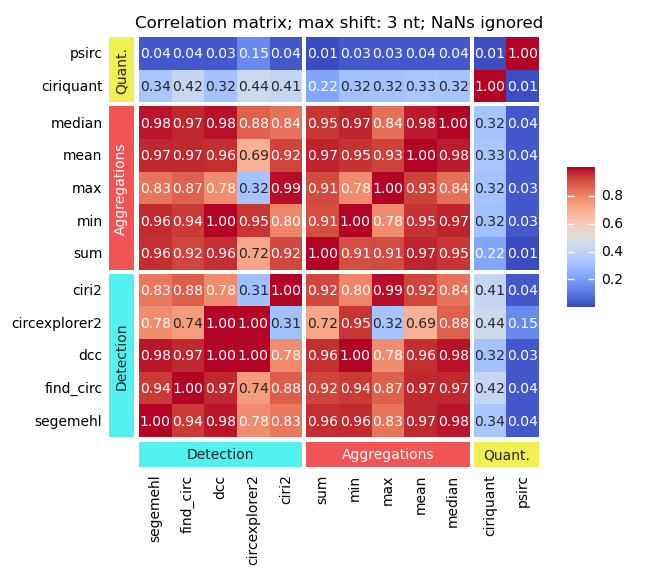
\includegraphics[width=\linewidth]{chapters/4_results_and_discussion/figures/quantification/correlation_heatmap_3_na.png}
            \caption{Missing values treated as NaN}
            \label{fig:correlation_heatmap_3_na}
        \end{subfigure} & \begin{subfigure}{0.5\textwidth} \centering

            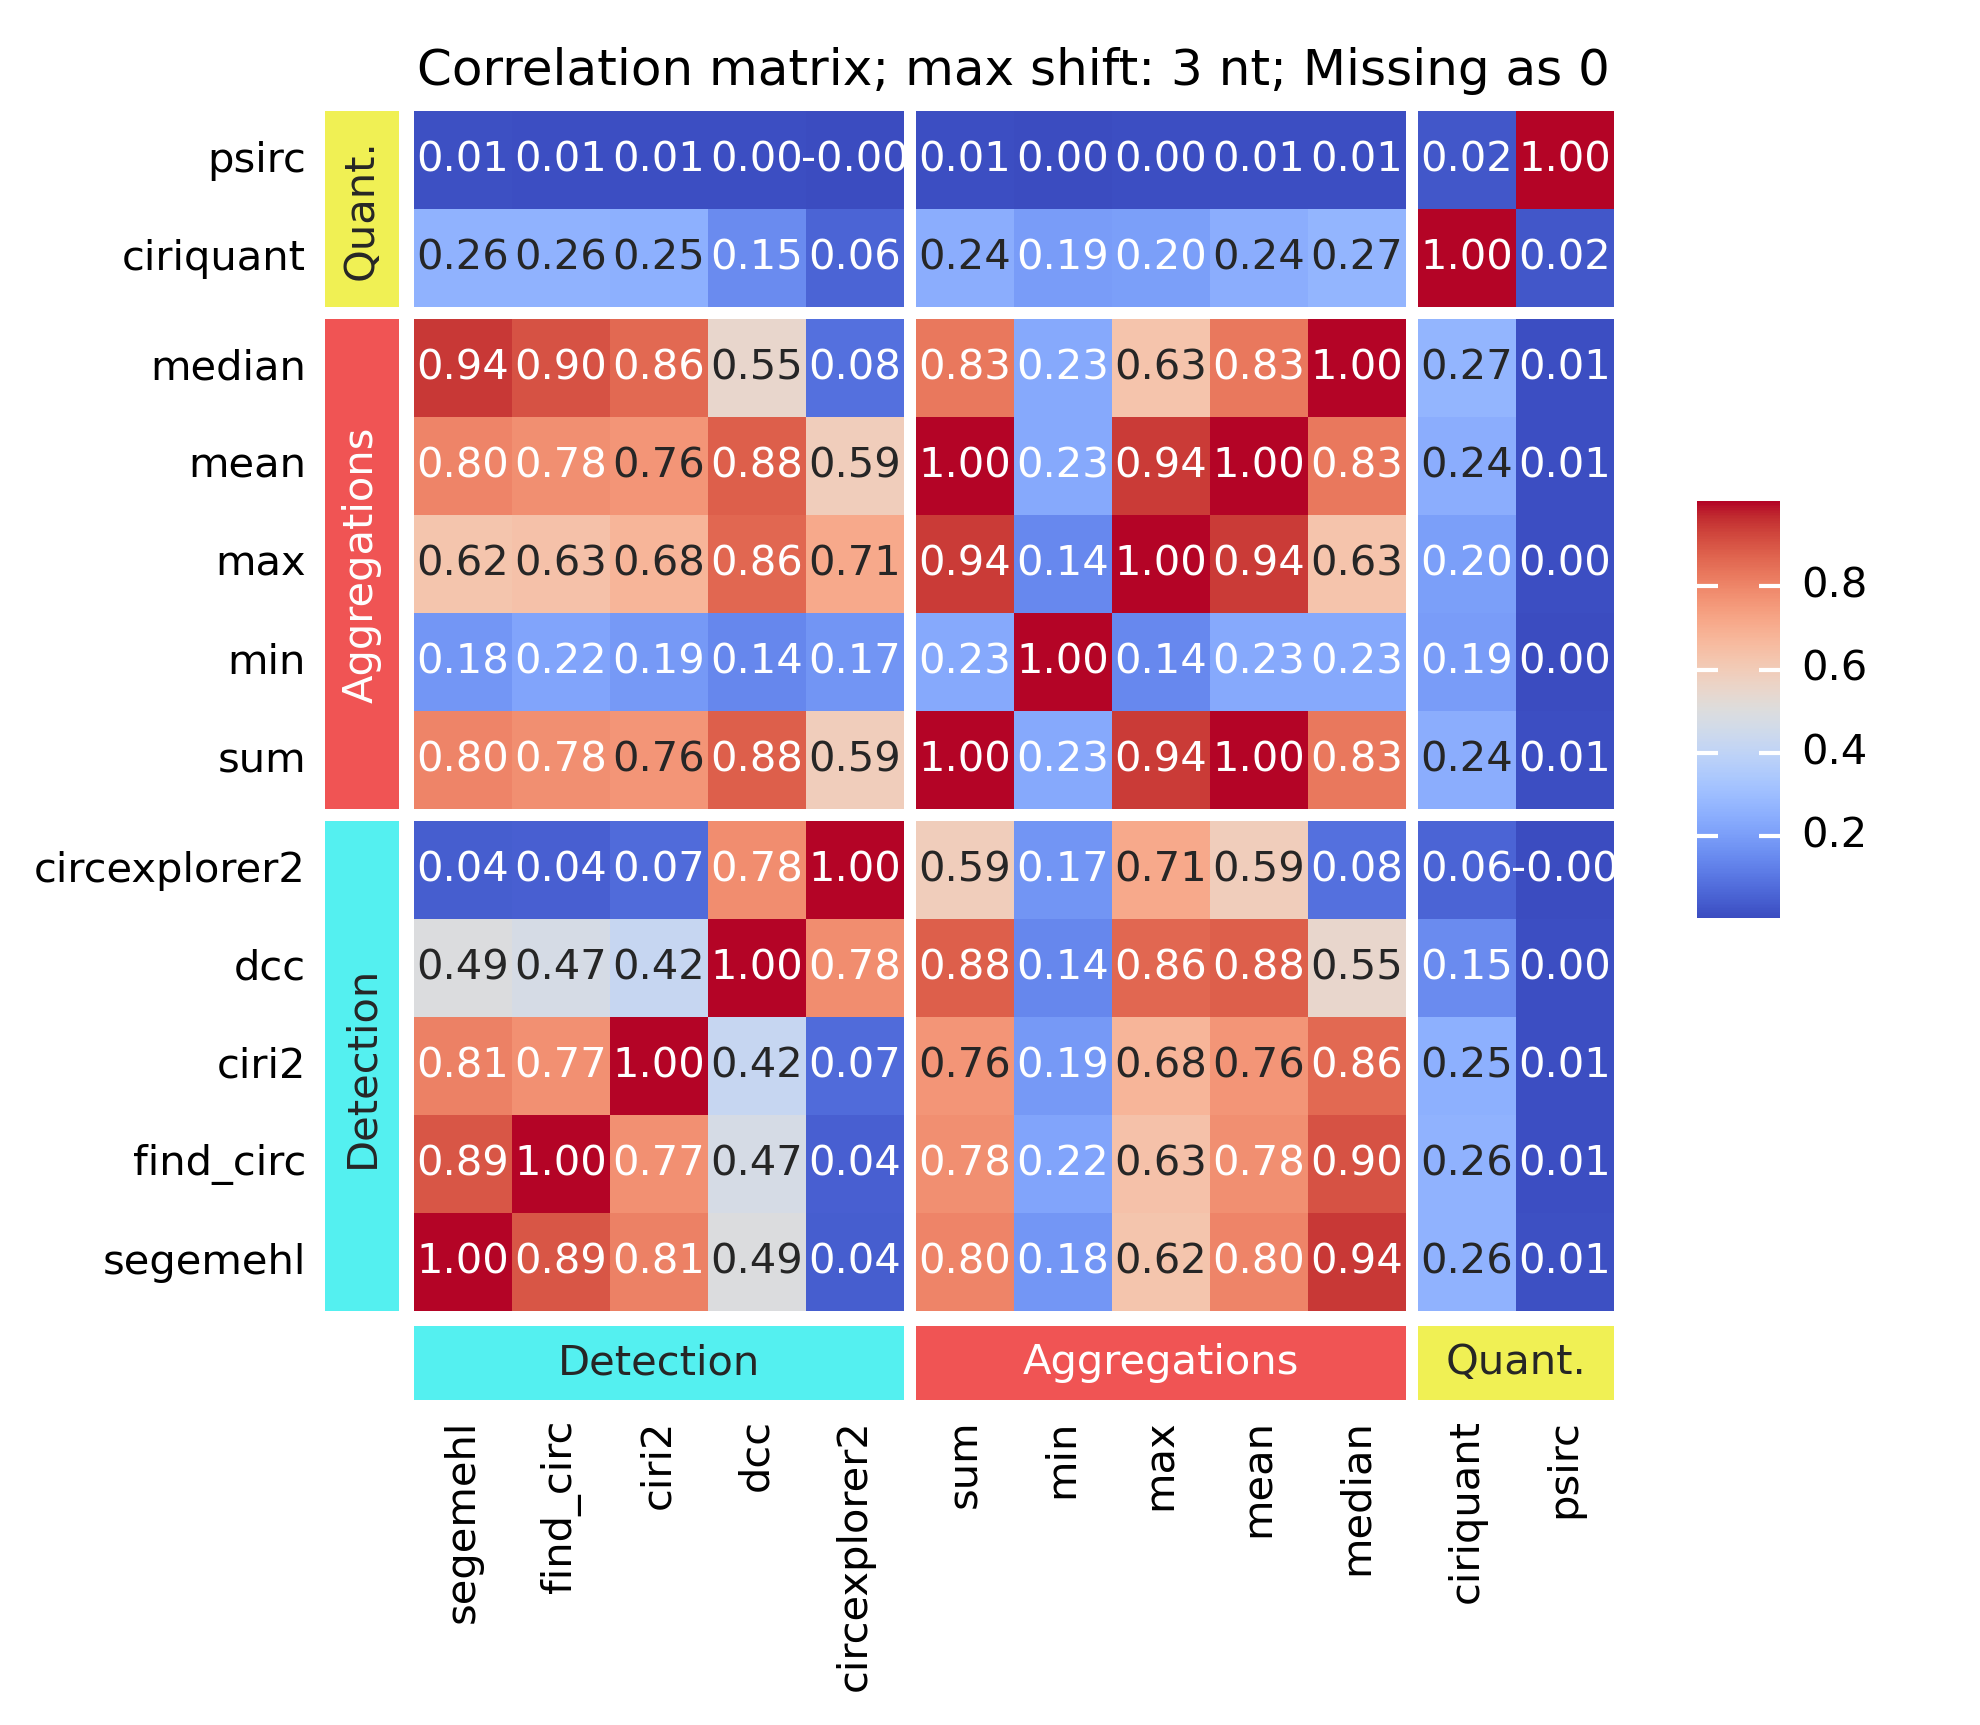
\includegraphics[width=\linewidth]{chapters/4_results_and_discussion/figures/quantification/correlation_heatmap_3_0.png}
            \caption{Missing values treated as 0}
            \label{fig:correlation_heatmap_3_0}
        \end{subfigure} \end{tabular} \caption{Pearson correlation heatmaps
        between the quantification results of the detection tools, multiple
        aggregations of the detection tools, and the quantification tools.
        The expression values were scaled so that the sum per sample and tool is
        constant.
        For each detected \gls{bsj}, expression information of all \glspl{bsj} within a
        \textit{max shift} of 3 on either strand was summed.
        \Cref{fig:correlation_heatmap_3_na} shows the correlation when treating
        missing values as NaN, while \cref{fig:correlation_heatmap_3_0} shows
        the
        correlation when treating missing values as 0.
    } \label{fig:correlation_heatmap} \end{figure}

As \cref{fig:correlation_heatmap} depicts, treating missing values as NaN
results in higher correlations overall.
However, treating the zeros as actual 0 values better reflects the underlying
biology.
This is because missing values mean that a tool did not detect any reads
supporting a \gls{bsj} (thus not outputting anything), which is equal to the
definition of 0 expression.

\subsubsection{Quantification tools}
Interestingly, the quantification tools show relatively low correlation with
the detection tools and aggregations.
While both show robust results in their respective publications, they were only
validated on paired end
data\supercite{zhang_accurate_2020,yu_quantifying_2021}.

\paragraph{\glsfmtlong{psirc-quant}}
For \gls{psirc-quant}, there is an additional complication: As mentioned in
\cref{sec:psirc}, it expects the full-length isoform \glspl{crna} sequence as
input.
As this study is based on single-end data, this information is not available.
Therefore, the entire sequence within the \gls{bsj} boundaries is used as the
\gls{crna} sequence.
While \gls{psirc-quant} uses the information that the sequence is circular when
constructing the \gls{t-dbg}, it does not treat reads spanning the \gls{bsj}
differently from reads that do not\supercite{yu_quantifying_2021}.

While due to the lack of ground truth it is impossible to say that the
quantification results of \gls{psirc-quant} are wrong, the low correlation with
the detection tools indicates that they are at least questionable in this
context.
Thus, I will not use the quantification results of \gls{psirc-quant} in the
following analyses.

\paragraph{\glsfmtlong{ciriquant}}
\Gls{ciriquant}, on the other hand, shows a higher correlation with
the detection tools and aggregations than \gls{psirc-quant}.
However, it is still relatively low ($<$0.35 in all comparisons when treating
missing values as 0).
Here, it is not clear why the correlation is so low, as \gls{ciriquant} uses a
similar approach to the detection tools.
Again, the lack of a ground truth makes it impossible to say whether the
quantification results of \gls{ciriquant} are trustworthy in this setting.

\subsubsection{Detection tools}
In \cref{fig:correlation_heatmap} it appears like there are two groups of
detection tools: One including \gls{segemehl}, \gls{findcirc} and \gls{ciri2},
and the other including DCC and \gls{cex2}.
Both show high internal correlation in both settings ($>$0.7) and low
correlation between the groups ($\leq$0.55).

A potential explanation for the high correlation between \gls{cex2} and
\gls{dcc} is that they are both based on the same alignment generated by
STAR\supercite{dobin_star_2013}.
The other tools each use a different alignment method.
This however does not explain the high internal correlation between
\gls{segemehl}, \gls{findcirc} and \gls{ciri2}.

\subsubsection{Aggregations}
Many of the investigated aggregations seem to be able to smoothen out the
differences between the two groups of detection tools.
In the following paragraphs, I will look into the individual aggregations in
more detail.

\paragraph{min}
Using the minimum expression value of all tools for each \gls{bsj}
interestingly results in high correlations with \gls{findcirc} and
\gls{segemehl} when treating missing values as NaN.
In this setting, the minimum expression will be the smallest value of tools
with an expression value.
When looking at the behaviour of the min aggregation when treating missing
values as 0, we see that all correlation values are $<$0.25.
Here, the min aggregation will be 0 if any of the tools did not detect any
reads supporting a \gls{bsj}, which is true for many \glspl{bsj}.

\paragraph{median}
The median aggregation shows a tendency to correlate with the
segemehl-\gls{findcirc}-\gls{ciri2} group.
This is not surprising, as this group consists of 3 tools whereas the
DCC-\gls{cex2} group consists of only 2 tools.
Thus, if all tools detect a \gls{bsj}, the median will be the lowest entry from
the first group.

\paragraph{max}
The max aggregation interestingly has high correlations with DCC and
\gls{cex2} in the NaN setting.
This indicates that - if they detect a \gls{bsj} - they often detect a high
number of reads supporting it.
In the 0 setting, the max aggregation achieved a correlation $\geq 0.55$ with
all tools, thus yielding stable, but slightly worse results than the following
aggregations.

\paragraph{sum}
The sum aggregation results in robust correlations in both settings.
While the correlation with \gls{cex2} is lower than with the other tools in
the 0 setting, this is mostly due to the fact that \gls{cex2} detects fewer
\glspl{bsj} than the other tools.
This is supported by the fact that \gls{cex2} has a high correlation of 0.96
in the NaN setting, where only \glspl{bsj} where \gls{cex2} detected reads
are considered.

\paragraph{mean}
This behaves very similarly to the sum aggregation.
Mathematically, the mean aggregation is the sum divided by the number of tools
with an expression value.
Thus, in the 0 setting, they are equal, while in the NaN setting, the mean
aggregation will deviate if a tool did not detect any reads supporting a
\gls{bsj}.

\subsection{Conclusion}

While psirc appears to be unsuitable for quantification if the full-length
\gls{crna} sequence is not available, \gls{ciriquant} at least shows some
correlation with the detection tools and aggregations.
As there is no ground truth available, both the sum aggregation and the
quantification results of \gls{ciriquant} will be considered in the following
analyses.

\section{Differential expression analysis}


\section{Biological interpretation}

\chapter{Conclusion and Outlook}

\appendix
\chapter{Appendix}

\begin{figure}[ht]
    \begin{tabular}{cc}
        \begin{subfigure}{\textwidth}
            \centering

            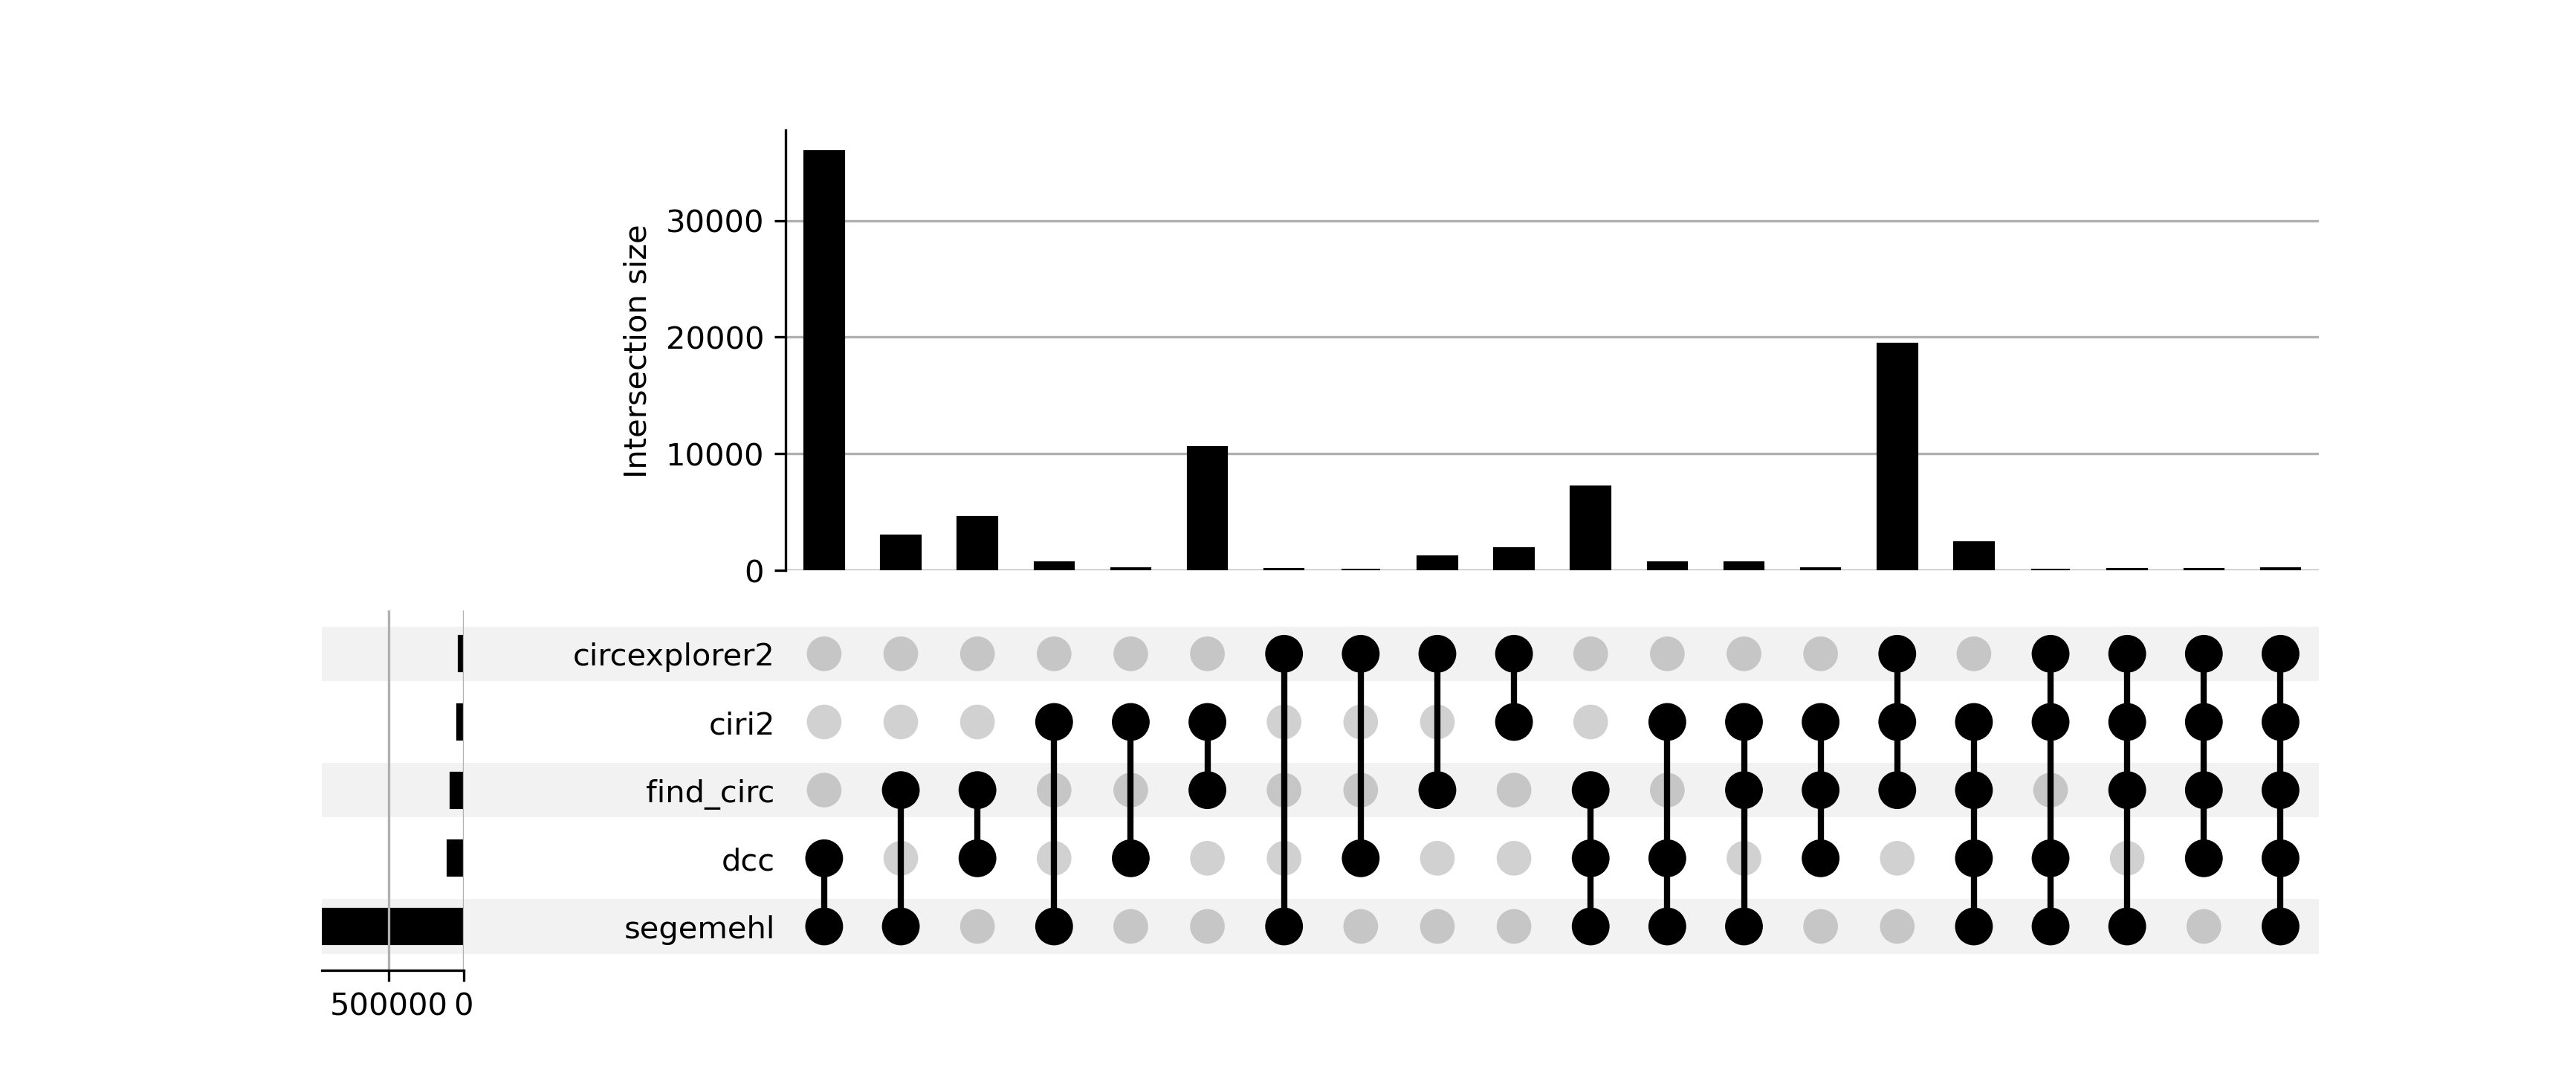
\includegraphics[width=\linewidth]{chapters/4_results_and_discussion/figures/detection/upset/diff_1_strand.png}
            \caption{Shift of 1 allowed, strand considered}
            \label{fig:detection_upset_1_strand}
        \end{subfigure}
        \\
        \begin{subfigure}{\textwidth}
            \centering

            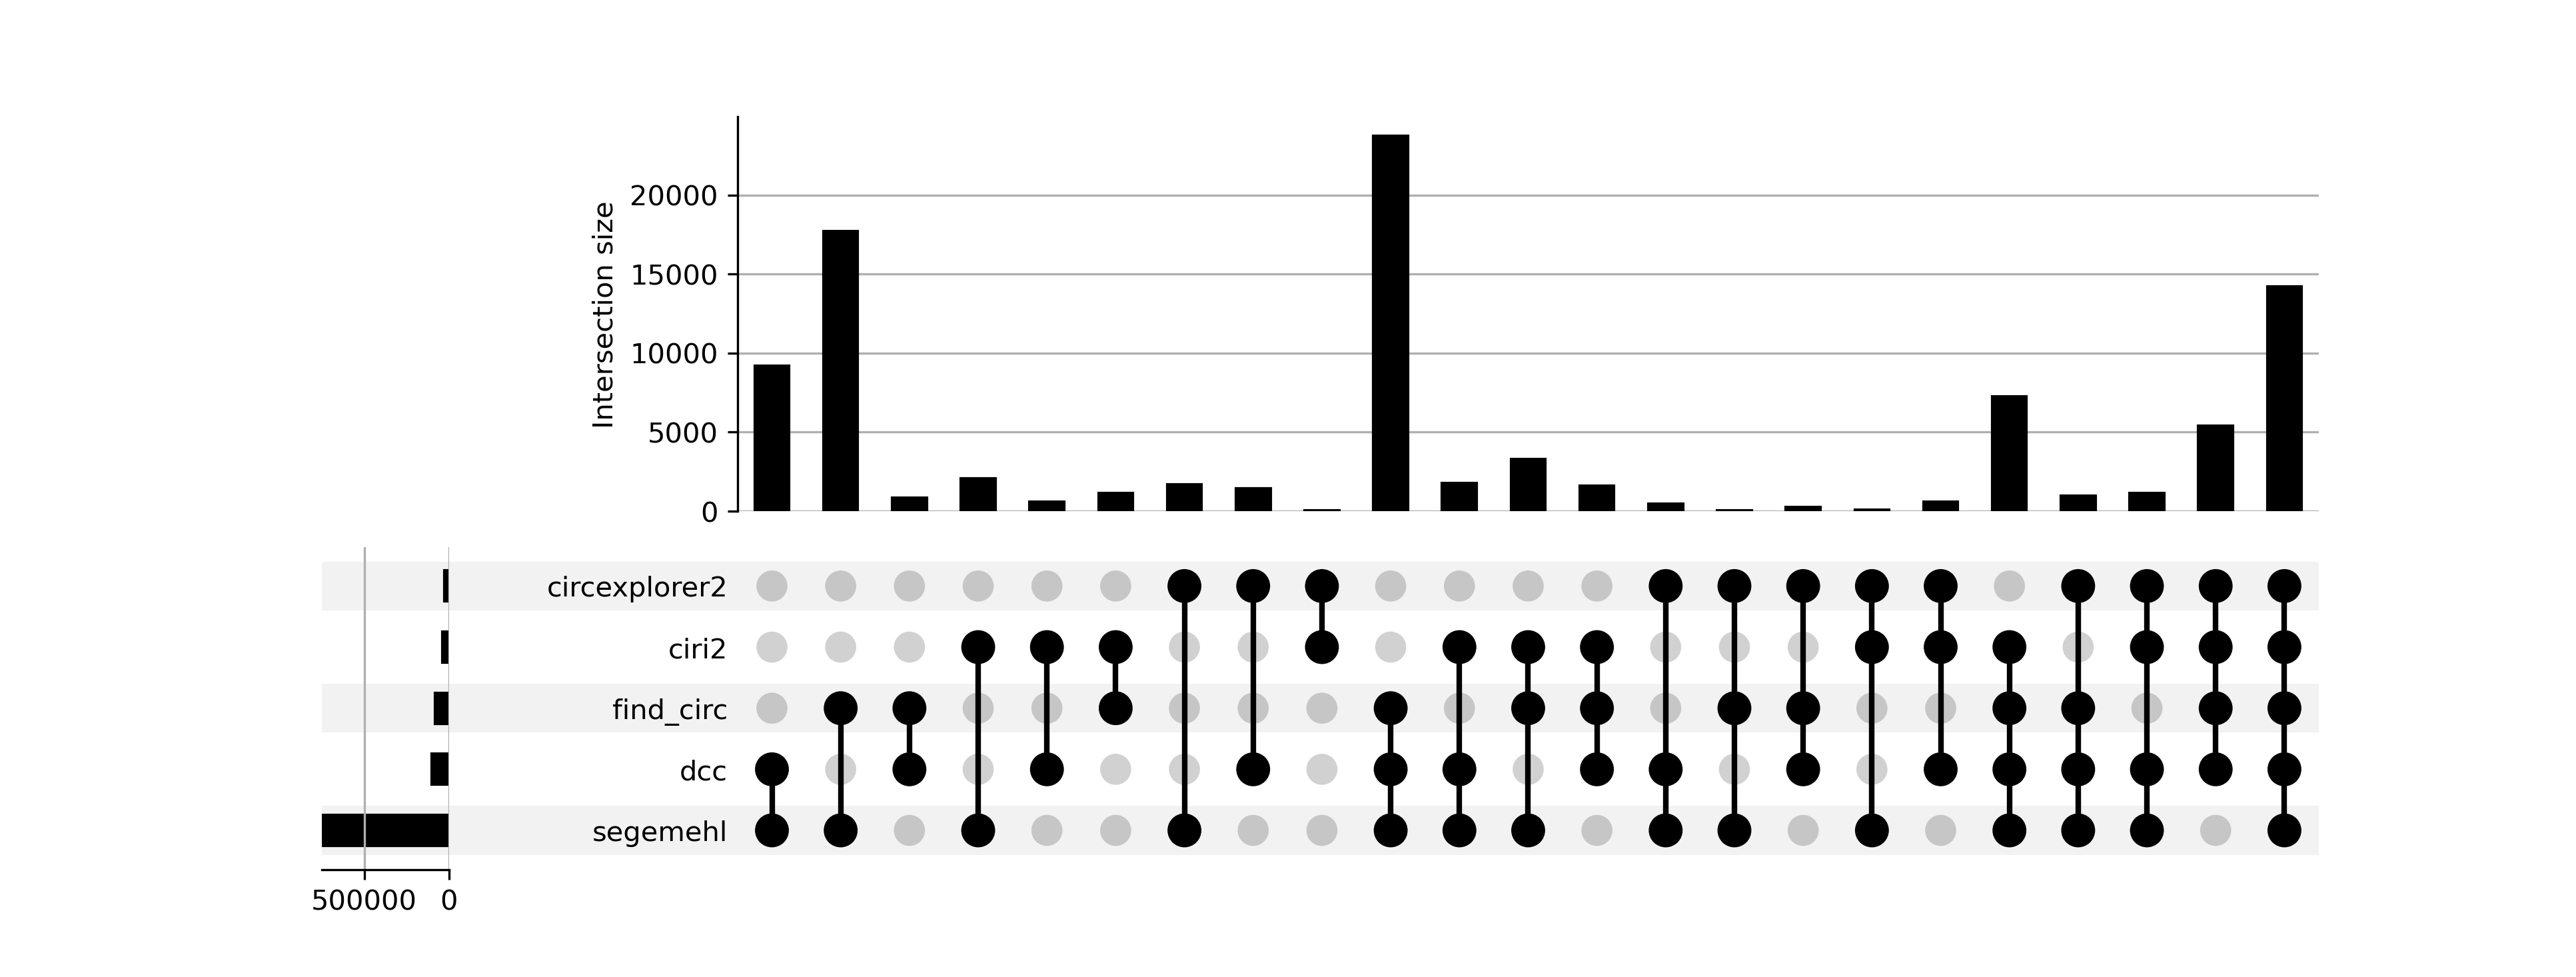
\includegraphics[width=\linewidth]{chapters/4_results_and_discussion/figures/detection/upset/diff_20_nostrand.png}
            \caption{Shift of 20 allowed, strand ignored}
            \label{fig:detection_upset_20_nostrand}
        \end{subfigure}
    \end{tabular}
    \caption{Upset plots
    }
    \label{fig:appendix_detection_upset}
\end{figure}


\backmatter

\printbibliography

\end{document}
